% =====================================================================
%  Linear Statistical Models -- Lecture Notes
%  Based on the IIT Madras BS course by Prof. Siva Athreya
% =====================================================================
\documentclass[11pt]{report}

% ---------------------------------------------------------------------
% lindrew.sty contains  \newcommand{\the}{\vartheta}.  \the is a TeX
% primitive, so that line raises "Command \the already defined" on every
% engine.  We do NOT edit the style file.  Instead, while (and only while)
% the package is loaded, the "not definable" error is turned into a
% warning; the offending definition is skipped and \the keeps its
% primitive meaning.  In the notes we write \vartheta directly.
% Delete the four lines around \usepackage to see the original error.
% ---------------------------------------------------------------------
\makeatletter
\let\LSM@savednotdefinable\@notdefinable
\def\@notdefinable{\PackageWarningNoLine{lindrew}{Skipped a \string\newcommand\space
  for an already-defined command (the \string\the\space line; see main.tex)}}
\makeatother
\usepackage[formal]{lindrew}
\makeatletter
\let\@notdefinable\LSM@savednotdefinable
\makeatother

% Book-wide macros (new names only; nothing from lindrew.sty is redefined)
\newcommand{\T}{^{\mathsf T}}                 % transpose
\newcommand{\colsp}[1]{\mc{C}\paren{#1}}      % column space
\newcommand{\nullsp}[1]{\mc{N}\paren{#1}}     % null space
\newcommand{\rowsp}[1]{\mc{R}\paren{#1}}      % row space
\newcommand{\PX}{P_X}                          % orthogonal projection onto C(X)
\newcommand{\one}{\mathbf 1}                   % vector of ones
\newcommand{\ginv}[1]{#1^{-}}                  % generalized inverse
\newcommand{\rank}{\operatorname{rank}}
\newcommand{\SSE}{\mathrm{SSE}}
\newcommand{\RSS}{\mathrm{RSS}}
\newcommand{\TSS}{\mathrm{TSS}}
\newcommand{\SSW}{\mathrm{SSW}}
\newcommand{\SSB}{\mathrm{SSB}}
\newcommand{\RSE}{\mathrm{RSE}}
\newcommand{\N}{\mathcal N}                    % normal distribution
\newcommand{\nb}[1]{\texttt{notebooks/#1}}     % pointer to a notebook
% Lecture header: {number}{youtube id}{source actually used}
\newcommand{\lectureheader}[3]{%
  \noindent\begin{tabular}{@{}lp{0.78\linewidth}@{}}
  \textbf{Lecture:} & #1\\
  \textbf{Video:} & \href{https://youtu.be/#2}{\texttt{\detokenize{https://youtu.be/#2}}}\\
  \textbf{Timestamps:} & not available (video transcript not accessed)\\
  \textbf{Source used:} & #3
  \end{tabular}\par\medskip}
\newcommand{\abs}[1]{\left|#1\right|}
% A displayed line of code that may wrap at spaces
\newcommand{\codeline}[1]{\par\smallskip\noindent\hspace*{1.5em}%
  \parbox{\dimexpr\linewidth-3em\relax}{\raggedright\ttfamily\small #1}\par\smallskip}
% Allow a little more stretch to avoid overfull lines with inline code
\emergencystretch=2.5em


\title{Linear Statistical Models\\[0.4em]
  \large Lecture notes and Python companion\\
  based on the IIT Madras BS Degree course by Prof.\ Siva Athreya}
\author{Compiled lecture notes}
\date{Part I: Weeks 1--5 (Lectures 1--18)}

\begin{document}
\maketitle
\tableofcontents
\chapter*{Notation}
\addcontentsline{toc}{chapter}{Notation}

The same notation is used throughout the book. Where the instructor's own
notation differs, the last column says how to translate.

\begin{center}
\renewcommand{\arraystretch}{1.25}
\begin{tabular}{@{}p{3.4cm}p{7.2cm}p{4.6cm}@{}}
\hline
\textbf{Symbol} & \textbf{Meaning} & \textbf{Instructor's notes}\\\hline
$Y = X\beta + \eps$ & the linear model; $Y\in\RR^n$ observed, $\beta\in\RR^p$ unknown & same, with $m$ parameters\\
$n$ & number of observations & same\\
$p$ & number of parameters (columns of $X$) & written $m$\\
$X$ & $n\times p$ known design matrix, $X=(x_{ij})$ & same\\
$r=\rank(X)$ & rank of the design matrix & --\\
$\eps$ & error vector, $\EE(\eps)=0$, $\Cov(\eps)=\sigma^2 I_n$ & same\\
$(Y,X\beta,\sigma^2 I_n)$ & shorthand for the linear model above & same\\
$\lambda\T\beta$ & a linear parametric function, $\lambda\in\RR^p$ & written $p\T\beta$, $p\in\RR^m$\\
$\ell\T Y$ & a linear estimator, $\ell\in\RR^n$ & same\\
$\colsp{A}$, $\nullsp{A}$, $\rowsp{A}$ & column space, null space, row space of $A$ & $\mc{C}(A)$, $\mc N(A)$, $\mc R(A)$\\
$\PX$ & orthogonal projection of $\RR^n$ onto $\colsp{X}$ & same\\
$\ginv{A}$ & a generalized inverse of $A$: $A\ginv{A}A=A$ & --\\
$\hat\beta$ & any solution of the normal equations $X\T X\beta = X\T Y$ & $\hat\beta$ or $\tilde\beta$\\
$\hat Y = X\hat\beta=\PX Y$ & fitted values & same\\
$\hat e = Y-\hat Y$ & residual vector & same\\
$\RSS=\SSE=\pnorm{Y-\hat Y}^2$ & residual (error) sum of squares & $R_0^2$\\
$\TSS$ & total sum of squares $\sum(Y_i-\bar Y)^2$ & same\\
$\SSW$, $\SSB$ & within- and between-group sums of squares & same\\
$\bar Y_{i\cdot}$, $\bar Y_{\cdot\cdot}$ & group mean and grand mean & same\\
$\one_n$ & the vector of $n$ ones & --\\
$\RR,\EE,\PP$ & reals, expectation, probability & --\\
$\Var,\Cov,\tr$ & variance, covariance, trace & --\\
$\N(\mu,\sigma^2)$ & normal distribution & Normal$(\mu,\sigma^2)$\\
$\chi^2_k$, $t_k$, $F_{k_1,k_2}$ & chi-square, Student-$t$ and $F$ distributions & same\\
$\indep$ & independence & --\\\hline
\end{tabular}
\end{center}

\paragraph{How to read these notes.}
Unmarked text follows the instructor's published material for the relevant week.
Boxes whose title begins with \emph{Supplementary} contain material added by the
compiler: extra proofs, intuition or examples that are not in that material. Each lecture
header states exactly which source was used. The video transcripts were
\emph{not} accessed. Because of that, video timestamps are not given, and the
order of topics follows the published notes.


% ============================================================
% Week 1 -- Review of basic statistics and working with R
% ============================================================
\chapter{Basic Statistics, R and Data Visualisation}\label{ch:week01}

This chapter covers Week~1 of the course (Lectures 1--3). The instructor's schedule starts
with the computing environment and exploratory graphics. The linear model itself appears in
Week~2. Note that the official syllabus lists ``Review of estimation, hypothesis testing''
for Week~1, but the published Week-1 material covers R and descriptive statistics. Estimation and
testing are reviewed when they are needed (\cref{sec:L08,sec:L16}).

% ============================================================
% Lecture 1 -- Basic Statistics and Introduction to R
% ============================================================
\section{Basic Statistics and Introduction to R}\label{sec:L01}

\lectureheader{1}{z1RfnVy8Oak}{Week-1 slides \texttt{Jan26notes.pdf} (with the instructor's handwritten annotations)}

\begin{guiding*}
By the end of this lecture you should be able to:
\begin{itemize}
  \item say what R is, where it came from, and how to install R and RStudio (and what the Python equivalents are);
  \item classify data as categorical, discrete numeric or continuous numeric;
  \item describe numerical data by its \emph{centre}, \emph{spread} and \emph{shape}, and compute the mean, median, mode, variance, standard deviation and inter-quartile range;
  \item load a built-in data frame, look at it with \texttt{head}, \texttt{tail} and indexing, and make the five-number summary, histogram and scatter plots.
\end{itemize}
\end{guiding*}

\subsection{Motivation}
The course is about \emph{linear statistical models}, but every model starts with data.
Before we write down $Y = X\beta+\eps$ we have to know how to read a data set, summarise it,
and draw pictures of it. The first week therefore reviews basic descriptive statistics and
introduces the computing environment. The instructor's slides open with a light-hearted
``statutory warning'': he tends to speak quickly, and students should ask him to repeat anything
that is unclear. The same advice applies to these notes: work through every example yourself,
in the companion notebook if you like.

\subsection{The R environment}
The slides describe R as follows.
\begin{itemize}
  \item R is an open-source programming language for statistical computing. It runs on Linux, Windows and Mac~OS, and it is free. The project web page is \url{http://www.r-project.org}.
  \item R is modelled on the languages S and S-Plus. S was developed in the late 1980s at AT\&T Bell Labs.
  \item The R project was started in 1995 by Robert Gentleman and Ross Ihaka of the Statistics Department of the University of Auckland (\emph{Journal of Computational and Graphical Statistics} 5:3, 299--314, 1996). It is now maintained by the R core development team with many contributors.
  \item R is downloaded from \url{https://cloud.r-project.org}. RStudio is an \vocab{integrated development environment} (IDE) for R.
\end{itemize}
There is plenty of help available on the web, for example the R-bloggers site.

\begin{note}[Supplementary: the Python counterpart used in this book]
Throughout these notes the R demonstrations are translated into Python. The ingredients are
\texttt{numpy} (arrays and linear algebra), \texttt{pandas} (data frames),
\texttt{matplotlib}/\texttt{seaborn} (graphics), \texttt{scipy.stats} (distributions) and
\texttt{statsmodels} (linear models). The IDE is VS~Code with the Jupyter extension. Setup
instructions are in the \texttt{README.md} at the root of the project.
\end{note}

\subsection{Kinds of data}
\begin{definition}[Types of data]\label{def:L01-datatypes}
The slides distinguish three kinds of data.
\begin{enumerate}
  \item \vocab{Categorical data}: each observation belongs to one of a set of labels, for example $\{0,1\}$ or $\{A,B,\dots\}$.
  \item \vocab{Discrete numeric data}: numbers that naturally take only discrete values, for example counts.
  \item \vocab{Continuous numeric data}: numbers that can take any value in an interval, for example temperature or a stock price.
\end{enumerate}
\end{definition}
The slides refer to S.\,S.~Stevens, ``On the theory of scales of measurement'',
\emph{Science} 103 (1946), 677--680, for a finer classification of measurement data. As typical
examples of numeric data the slides mention daily temperatures and the earnings of a stock in a
stock market. Such data are visualised with histograms and boxplots.

\begin{note}[Supplementary: Stevens' scales]
Stevens' paper is best known for its four scales of measurement: \emph{nominal} (labels only),
\emph{ordinal} (labels with an order), \emph{interval} (differences are meaningful, zero is
arbitrary, e.g.\ temperature in $^\circ$F) and \emph{ratio} (a true zero, e.g.\ length). The
scale determines which summaries make sense. A mean of nominal codes is meaningless, and a
ratio of two Fahrenheit temperatures has no physical meaning.
\end{note}

\subsection{Centre, spread and shape}
For numerical data the slides single out three key features. We make each one precise. Let
$x_1,\dots,x_n$ be the data and $x_{(1)}\le\dots\le x_{(n)}$ the ordered data.

\begin{definition}[Measures of centre]\label{def:L01-centre}
\begin{itemize}
  \item The \vocab{mean} (average) is $\bar x = \frac1n\sum_{i=1}^n x_i$. If the distinct values $x_1,\dots,x_k$ occur with frequencies $f_1,\dots,f_k$ ($\sum f_i=n$), then $\bar x = \frac1n\sum_{i=1}^k f_ix_i$. This frequency form is written on the slide.
  \item The \vocab{median} is the middle ordered value: $x_{((n+1)/2)}$ if $n$ is odd, and $\tfrac12\paren{x_{(n/2)}+x_{(n/2+1)}}$ if $n$ is even.
  \item The \vocab{mode} is the most frequently occurring value.
\end{itemize}
\end{definition}

\begin{definition}[Measures of spread]\label{def:L01-spread}
\begin{itemize}
  \item The (sample) \vocab{variance} is $s^2=\frac{1}{n-1}\sum_{i=1}^n (x_i-\bar x)^2$. This is R's \texttt{var}. The \vocab{standard deviation} is $s=\sqrt{s^2}$ (R's \texttt{sd}).
  \item The \vocab{inter-quartile range} is $\mathrm{IQR}=Q_3-Q_1$, where $Q_1$ and $Q_3$ are the first and third quartiles (the $25\%$ and $75\%$ quantiles).
\end{itemize}
\end{definition}

The \emph{shape} of the data describes, for example, whether it is symmetric or skewed about its
centre, and which values are more likely than others. The instructor's sketch shows a
symmetric histogram around $0$ and an asymmetric one with a long tail. Next to the sketch he
writes that most of the data lie in an ``essential range'' from mean$-3\,$SD to mean$+3\,$SD.
The next result makes this precise for \emph{every} data set.

\begin{proposition}[Supplementary: Chebyshev's inequality for data]\label{prop:L01-cheb}
Let $\sigma_n^2=\frac1n\sum (x_i-\bar x)^2$ and suppose $\sigma_n>0$. For every $k>0$, the proportion of data points with
$\abs{x_i-\bar x}\ge k\sigma_n$ is at most $1/k^2$. In particular at least $8/9\approx 89\%$ of any
data set lies within $3\sigma_n$ of the mean.
\end{proposition}
\begin{proof}
Let $A=\{i:\abs{x_i-\bar x}\ge k\sigma_n\}$ and let $\# A$ be its size. Every term in the sum below
is non-negative, and for $i\in A$ we have $(x_i-\bar x)^2\ge k^2\sigma_n^2$. Therefore
\[
n\sigma_n^2=\sum_{i=1}^n (x_i-\bar x)^2 \;\ge\; \sum_{i\in A}(x_i-\bar x)^2\;\ge\; \#A\cdot k^2\sigma_n^2 .
\]
Dividing by $nk^2\sigma_n^2>0$ gives $\#A/n\le 1/k^2$. Taking $k=3$ gives the second statement.
\end{proof}

For roughly bell-shaped data the proportion inside mean $\pm 3\,$SD is much higher, about
$99.7\%$. That is why the instructor calls it the essential range.

\begin{proposition}[Supplementary: the mean and the median as best constants]\label{prop:L01-bestconst}
For data $x_1,\dots,x_n$,
\begin{enumerate}
  \item $c\mapsto\sum_{i=1}^n (x_i-c)^2$ is minimised uniquely at $c=\bar x$;
  \item $c\mapsto\sum_{i=1}^n \abs{x_i-c}$ is minimised at any median.
\end{enumerate}
\end{proposition}
\begin{proof}
(1) Write $x_i-c=(x_i-\bar x)+(\bar x-c)$ and expand:
\[
\sum_{i}(x_i-c)^2=\sum_i (x_i-\bar x)^2 + 2(\bar x-c)\sum_i (x_i-\bar x) + n(\bar x-c)^2 .
\]
The middle sum is $\sum_i x_i - n\bar x=0$. So $\sum(x_i-c)^2=\sum(x_i-\bar x)^2+n(\bar x-c)^2$,
which is smallest exactly when $c=\bar x$.

(2) Let $g(c)=\sum_i\abs{x_i-c}$. The function $g$ is convex and piecewise linear. At a point $c$
that is not a data value its derivative is $\#\{i:x_i<c\}-\#\{i:x_i>c\}$. This is negative while
fewer than half of the points lie below $c$ and positive once more than half do. A convex
function is minimised where its slope changes sign, which is at a median.
\end{proof}
The first identity, ``total squared deviation $=$ deviation about the mean $+$ $n\times$(distance
of the mean)$^2$'', is the simplest case of the Pythagorean decompositions behind all of least
squares. We will meet it again in \cref{sec:L08,sec:L12}.

\begin{example}[Summaries by hand]\label{ex:L01-summary}
Consider the nine observations $3,7,8,5,12,14,21,13,18$.
\end{example}
\noindent\emph{Solution.} Ordered: $3,5,7,8,12,13,14,18,21$.
\begin{itemize}
  \item Mean: $\sum x_i=101$, so $\bar x=101/9=11.2222$.
  \item Median: $n=9$ is odd, so the median is $x_{(5)}=12$.
  \item Variance: $\sum x_i^2 = 9+25+49+64+144+169+196+324+441=1421$. Hence
  $\sum (x_i-\bar x)^2=\sum x_i^2-n\bar x^2 = 1421-101^2/9 = 1421-1133.4444=287.5556$, and
  $s^2=287.5556/8=35.9444$, $s=5.9954$.
  \item Quartiles: R's default rule (\texttt{type = 7}, also NumPy's default) puts the $q$-quantile at
  ordered position $1+(n-1)q$. For $q=0.25$ this is position $3$, so $Q_1=x_{(3)}=7$. For $q=0.75$ it is
  position $7$, so $Q_3=x_{(7)}=14$. Hence $\mathrm{IQR}=7$.
  \item The five-number summary is $(\min,Q_1,\text{median},Q_3,\max)=(3,7,12,14,21)$ and the mean is $11.22$.
  The mean is below the median here: the lower tail ($3,5$) pulls it down more than the upper tail pushes it up.
\end{itemize}
These numbers are reproduced in the notebook \nb{week01/L01\_basic\_stats\_intro.ipynb}.

\subsection{Data sets and data frames}
R ships with many data sets. The command \texttt{data()} lists the installed ones, and the
instructor strongly encourages students to pick a data set and repeat the class experiments on it.

\begin{definition}[Data frame]\label{def:L01-dataframe}
A \vocab{data frame} is a rectangular collection of \emph{variables} (the columns) and
\emph{observations} (the rows).
\end{definition}

\begin{example}[The \texttt{airquality} data]\label{ex:L01-airquality}
\texttt{?airquality} describes daily air-quality measurements in New York (May--September 1973).
It is a data frame with $153$ rows and $6$ columns: \texttt{Ozone}, \texttt{Solar.R}, \texttt{Wind},
\texttt{Temp}, \texttt{Month} and \texttt{Day}. The slides use it to show the following commands.
\begin{itemize}
  \item \texttt{head(airquality)} and \texttt{tail(airquality)} show the first and the last six rows; with \texttt{n = 10}, \texttt{head} shows ten rows.
  \item \texttt{airquality[148,4]} returns \texttt{63}, the entry in row 148 and column 4 (\texttt{Temp}). The same value is \texttt{airquality\$Temp[148]}.
  \item \texttt{airquality[148,]} is the whole 148th row. \texttt{airquality[,c(1,4)]} gives the \texttt{Ozone} and \texttt{Temp} columns for all rows; \texttt{c()} builds the vector of column numbers.
  \item \texttt{summary(airquality\$Temp)} prints the five-number summary together with the mean:
  \[
  \text{Min }56,\quad Q_1\ 72,\quad \text{Median }79,\quad \text{Mean }77.88,\quad Q_3\ 85,\quad \text{Max }97.
  \]
\end{itemize}
\end{example}

\begin{note}[Indexing pitfall]
R counts from $1$, Python from $0$. In pandas, R's \texttt{airquality[148,4]} is
\texttt{aq.iloc[147, 3]} or \texttt{aq.loc[147, "Temp"]}. The value is again $63$.
\end{note}

\subsection{First plots}
The slides then make three kinds of plot.
\begin{itemize}
  \item \texttt{hist(airquality\$Temp)}: a histogram. Temperatures range from $56$ to $97$ with a peak in the high $70$s and low $80$s, and the histogram is mildly left-skewed.
  \item \texttt{plot(airquality\$Temp)}: the values plotted against their index. Because the rows are in date order, this is a time plot. It shows temperatures rising into the summer and falling in September.
  \item \texttt{plot(airquality\$Ozone, airquality\$Temp)}: a scatter plot. Days with higher ozone tend to be hotter.
  \item \texttt{plot(airquality)}: a matrix of scatter plots of every pair of variables.
\end{itemize}

\begin{figure}[ht]
\centering
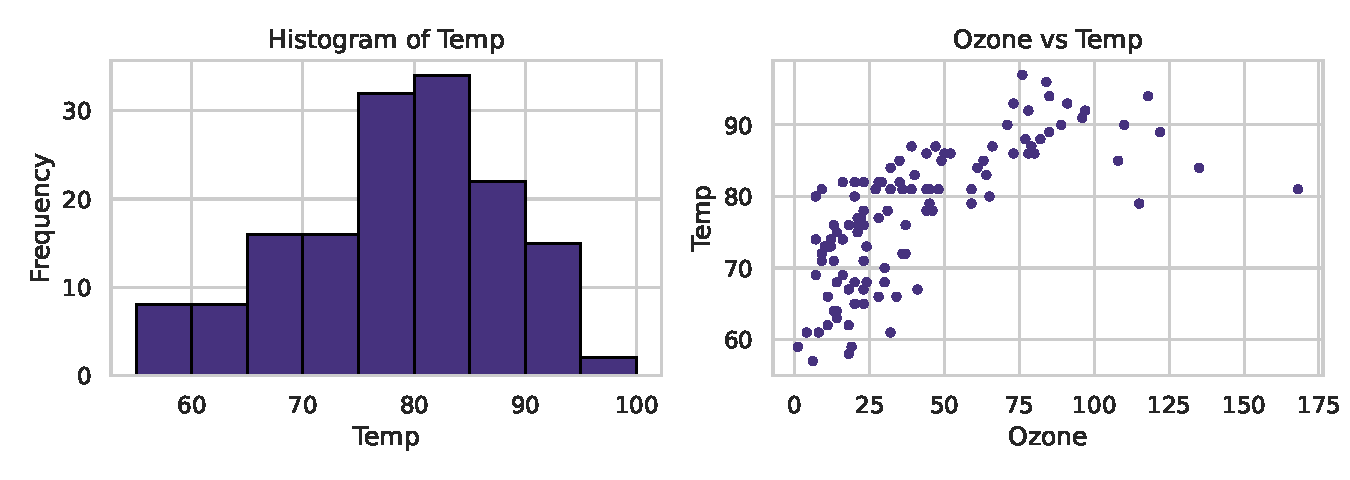
\includegraphics[width=0.95\textwidth]{figures/L01_airquality.pdf}
\caption{Histogram of \texttt{Temp} and scatter plot of \texttt{Temp} against \texttt{Ozone} (\texttt{airquality}).}
\label{fig:L01-airquality}
\end{figure}

\subsection{External packages}
R can be extended with packages. \texttt{install.packages("UsingR")} installs the package
\texttt{UsingR}, which contains many data sets, and \texttt{library("UsingR")} adds it to the
current workspace. Likewise \texttt{install.packages("tidyverse")} and
\texttt{library("tidyverse")} load \texttt{ggplot2}, the graphics system used in
\cref{sec:L02,sec:L03}.

\subsection{Computation}
The R commands of this lecture translate to Python as follows.
\begin{center}
\begin{tabular}{@{}ll@{}}\hline
R & Python (pandas / matplotlib)\\\hline
\texttt{head(airquality, n=10)} & \texttt{aq.head(10)}\\
\texttt{airquality[148,4]} & \texttt{aq.iloc[147, 3]}\\
\texttt{airquality[,c(1,4)]} & \texttt{aq.iloc[:, [0, 3]]}\\
\texttt{summary(airquality\$Temp)} & \texttt{aq.Temp.describe()}\\
\texttt{hist(airquality\$Temp)} & \texttt{plt.hist(aq.Temp)}\\
\texttt{plot(airquality)} & \texttt{pd.plotting.scatter\_matrix(aq)}\\\hline
\end{tabular}
\end{center}
Everything, including \cref{ex:L01-summary}, is in \nb{week01/L01\_basic\_stats\_intro.ipynb}.

\subsection{Summary}
\begin{itemize}
  \item R is a free language for statistics. The Python stack \texttt{pandas}/\texttt{statsmodels} does the same job in these notes.
  \item Data are categorical, discrete numeric or continuous numeric.
  \item Centre: $\bar x$, median, mode. Spread: $s^2=\frac{1}{n-1}\sum(x_i-\bar x)^2$, $s$, IQR. Shape: symmetry, skewness.
  \item $\sum(x_i-c)^2=\sum(x_i-\bar x)^2+n(\bar x-c)^2$, so the mean is the least-squares constant.
  \item A data frame has variables as columns and observations as rows. Use \texttt{head}, \texttt{tail}, indexing and \texttt{summary} to look at it, and histograms and scatter plots to picture it.
\end{itemize}

\subsection{Exercises}
\begin{problem}\label{prob:L01-1}
For the data $2,4,4,5,7,9,11$ compute the mean, median, mode, sample variance and IQR (using R's default quantile rule).
\end{problem}
\begin{problem}\label{prob:L01-2}
Show that $\sum_{i=1}^n (x_i-\bar x)^2=\sum_{i=1}^n x_i^2-n\bar x^2$.
\end{problem}
\begin{problem}\label{prob:L01-3}
Let $y_i=a+bx_i$ for constants $a,b$. Express $\bar y$, $s_y^2$ and $\mathrm{IQR}_y$ in terms of the corresponding quantities for $x$.
\end{problem}
\begin{problem}\label{prob:L01-4}
Using \texttt{airquality}, find the mean \texttt{Temp} for each month. Which month is hottest? (Use \texttt{groupby} in pandas.)
\end{problem}
\begin{problem}\label{prob:L01-5}
Give a data set of $10$ numbers in which fewer than $90\%$ of the observations lie within $2\sigma_n$ of the mean, and check that it still obeys \cref{prop:L01-cheb} with $k=2$.
\end{problem}

\subsection{Further reading}
Christensen does not cover exploratory data analysis. For this lecture see instead the
instructor's references: Verzani, \emph{simpleR} (Sections 13--15), and Wickham \& Grolemund,
\emph{R for Data Science}, Chapter~3. In Rao's \emph{Linear Statistical Inference}, the sample
moments appear in Chapter~2 (with the distribution of the sample mean and variance under
normality in Chapter~3).

% ============================================================
% Lecture 2 -- Data Visualization using ggplot2
% ============================================================
\section{Data Visualization using ggplot2}\label{sec:L02}

\lectureheader{2}{7nmwfGpgDkM}{Week-1 slides \texttt{Jan26notes.pdf}, ggplot2 part (slides on aesthetics, scaling, viridis, facets)}

\begin{guiding*}
By the end of this lecture you should be able to:
\begin{itemize}
  \item explain the idea of a \emph{grammar of graphics} and the basic \texttt{ggplot} template;
  \item map a variable to an \emph{aesthetic} (colour, shape, size) and explain what \emph{scaling} does;
  \item use colour-blind-safe \emph{viridis} palettes;
  \item split a plot into \emph{facets} with \texttt{facet\_wrap} and \texttt{facet\_grid};
  \item reproduce all of these plots in Python with \texttt{seaborn}/\texttt{matplotlib}.
\end{itemize}
\end{guiding*}

\subsection{Recap and motivation}
In \cref{sec:L01} we used R's base graphics (\texttt{hist}, \texttt{plot}). They are quick, but
each kind of plot has its own function with its own arguments. The package \texttt{ggplot2}
(loaded by \texttt{library(tidyverse)}) takes a different route: it is built on a \emph{grammar
of graphics}. The instructor's annotation sums up the benefit: ``a system for describing and
building graphs --- learn one system and apply it at many places''. In linear models we
constantly plot a response against predictors, coloured or split by a factor. This is exactly
what the grammar makes easy.

\subsection{The \texttt{mpg} data}
The running example is the tidyverse data set \texttt{mpg}. It contains observations collected
by the US Environmental Protection Agency on $38$ models of cars ($234$ rows, $11$ columns).
Two variables matter most here:
\begin{itemize}
  \item \texttt{displ}: engine displacement in litres (the car's engine size);
  \item \texttt{hwy}: fuel efficiency on the highway, in miles per gallon.
\end{itemize}
Other variables used below are \texttt{class} (type of car: 2seater, compact, midsize, minivan,
pickup, subcompact, suv), \texttt{drv} (\texttt{f} = front-wheel, \texttt{r} = rear-wheel,
\texttt{4} = four-wheel drive), \texttt{cyl} (number of cylinders) and \texttt{trans} (type of
transmission).

\subsection{The basic template}
The first plot on the slides is
\codeline{ggplot(data = mpg) + geom\_point(mapping = aes(x = displ, y = hwy))}
It shows a \emph{negative relationship between engine size and fuel efficiency}: cars with big
engines use more fuel.

\begin{definition}[The ggplot template]\label{def:L02-template}
A \texttt{ggplot2} graph is built in layers:
\begin{enumerate}
  \item \texttt{ggplot(data = <DATA>)} creates a coordinate system to which layers are added. On its own it draws an empty graph.
  \item A \vocab{geom function} such as \texttt{geom\_point()} adds a layer, here a layer of points.
  \item Each geom takes a \texttt{mapping} argument, which is always paired with \texttt{aes()}. It says which variables go on which visual channels.
\end{enumerate}
In short: \texttt{ggplot(data = <DATA>) + <GEOM\_FUNCTION>(mapping = aes(<MAPPINGS>))}.
\end{definition}

\subsection{Aesthetic mappings and scaling}
\begin{definition}[Aesthetic, mapping, scaling]\label{def:L02-aes}
An \vocab{aesthetic} is a visual property of the objects in the plot: position ($x$, $y$),
\texttt{colour}, \texttt{shape}, \texttt{size}, and so on. To \vocab{map} a variable to an
aesthetic we associate the aesthetic's name with the variable's name inside \texttt{aes()}.
\vocab{Scaling} is the step in which \texttt{ggplot2} assigns a unique level of the aesthetic
(a colour, say) to each unique level of the variable. It also adds a legend that explains the
correspondence.
\end{definition}

\begin{example}[Adding a third variable]\label{ex:L02-colour}
\texttt{ggplot(data=mpg) + geom\_point(mapping=aes(x=displ, y=hwy, colour=class))} adds the
variable \texttt{class} to the two-dimensional scatter plot by mapping it to the aesthetic
\texttt{colour}. Here the aesthetic's name is \texttt{colour} and the variable is
\texttt{class}. Scaling assigns $7$ colours to the $7$ classes, and the legend lists them.
The plot shows that most of the cars with large engines but unusually \emph{good} mileage are
\texttt{2seater}s. These are sports cars: big engines, but light bodies.
\end{example}
Other aesthetics include \texttt{shape} and \texttt{size}. The instructor notes on the slide
that one can add \texttt{shape} in exactly the same way.

\begin{figure}[ht]
\centering
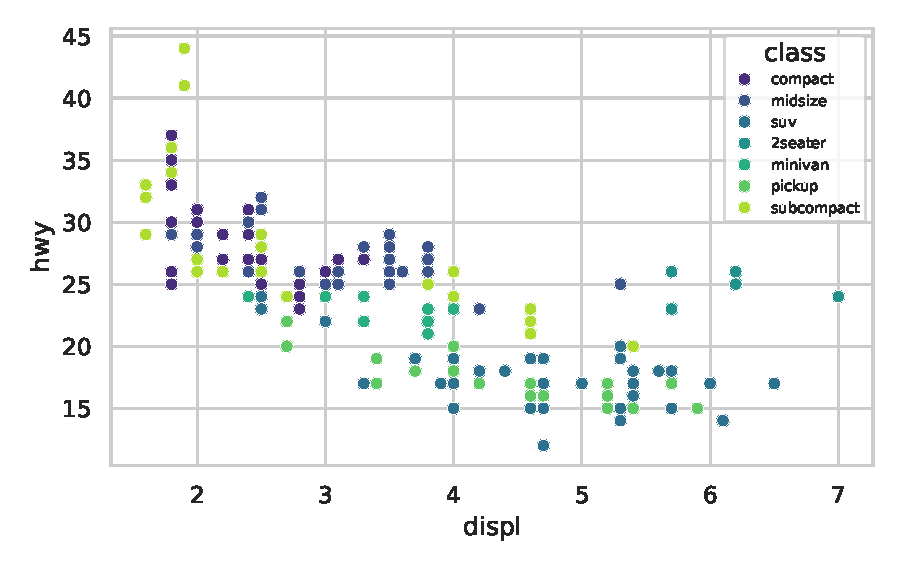
\includegraphics[width=0.7\textwidth]{figures/L02_mpg_class.pdf}
\caption{\texttt{hwy} against \texttt{displ}, coloured by \texttt{class} (viridis palette).}
\label{fig:L02-class}
\end{figure}

\begin{note}[Supplementary: mapping versus setting]
Putting \texttt{colour = class} \emph{inside} \texttt{aes()} maps a variable to colour. Putting
\texttt{colour = "blue"} \emph{outside} \texttt{aes()} just sets every point to blue. A common
beginner's mistake is \texttt{aes(colour = "blue")}. This maps a constant \emph{variable} whose
single level is the string \texttt{"blue"}, so the points get the first default colour
(pinkish-red) and a pointless legend appears.
\end{note}

\subsection{Viridis colour scales}
The viridis scales give colour maps that are \emph{perceptually uniform} in both colour and
black-and-white. They are also designed to be read correctly by viewers with common forms of
colour blindness (see \url{https://bids.github.io/colormap/}). Adding
\texttt{+ scale\_colour\_viridis\_d()} to the previous plot switches to the default viridis
palette for a discrete variable. \texttt{scale\_colour\_viridis\_d(option = "plasma")} chooses
the ``plasma'' variant.

\subsection{Facets}
Aesthetics are one way to add a variable. Another, especially useful for categorical variables,
is to split the plot into \vocab{facets}.

\begin{definition}[Facets]\label{def:L02-facets}
\texttt{facet\_wrap(\textasciitilde\ class, nrow = 2)} splits a plot by a \emph{single} variable
into subplots, each showing one subset of the data. \texttt{facet\_grid(drv \textasciitilde\ cyl)}
splits by the \emph{combination} of two variables: rows are levels of \texttt{drv}, columns are
levels of \texttt{cyl}.
\end{definition}

\begin{example}[Facets on \texttt{mpg}]\label{ex:L02-facets}
With \texttt{facet\_wrap(\textasciitilde class, nrow=2)} we get seven panels. The pickup and SUV
panels show large engines and low mileage, while the compact and subcompact panels contain the
high-mileage cars. With \texttt{facet\_grid(drv\textasciitilde cyl)} the $3\times 4$ grid shows,
for instance, that there are \emph{no} rear-wheel-drive cars with $4$ or $5$ cylinders in the
data. Those cells are empty. Facets and colour can be combined, as on the last slide of this
part:
\texttt{geom\_point(aes(colour=class)) + scale\_colour\_viridis\_d(option="plasma") + facet\_wrap(\textasciitilde class, nrow=2)}.
\end{example}

\begin{figure}[ht]
\centering
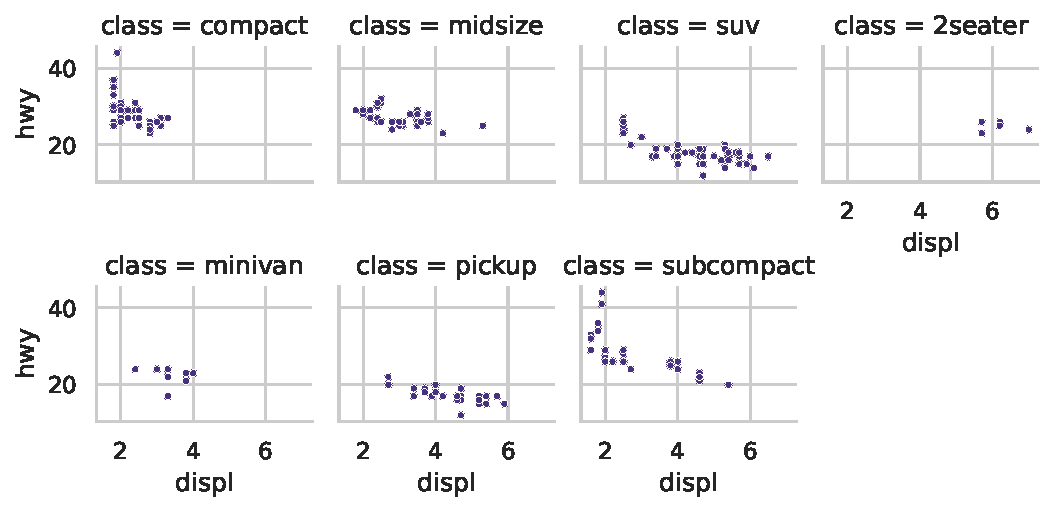
\includegraphics[width=0.95\textwidth]{figures/L02_mpg_facets.pdf}
\caption{\texttt{facet\_wrap(\textasciitilde\ class)}: one panel per class.}
\label{fig:L02-facets}
\end{figure}

\begin{note}[Supplementary: why facets matter for linear models]
In a regression of \texttt{hwy} on \texttt{displ}, the relationship could differ between
classes. For example, the slope within SUVs could differ from the slope within compacts.
Faceting by a factor is the visual version of fitting a model with a
\emph{factor $\times$ covariate interaction}. That is the analysis of covariance (ANCOVA), which
comes later in the course.
\end{note}

\subsection{Computation}
\begin{center}
\small\begin{tabular}{@{}>{\raggedright\arraybackslash}p{7.3cm}>{\raggedright\arraybackslash}p{8.3cm}@{}}\hline
R (\texttt{ggplot2}) & Python (\texttt{seaborn})\\\hline
\texttt{ggplot(mpg)+geom\_point(aes(displ,hwy))} & \texttt{sns.scatterplot(data=mpg, x="displ", y="hwy")}\\
\texttt{aes(..., colour=class)} & \texttt{hue="class"}\\
\texttt{scale\_colour\_viridis\_d()} & \texttt{palette="viridis"}\\
\texttt{option="plasma"} & \texttt{palette="plasma"}\\
\texttt{facet\_wrap(\textasciitilde class, nrow=2)} & \texttt{sns.relplot(..., col="class", col\_wrap=4)}\\
\texttt{facet\_grid(drv\textasciitilde cyl)} & \texttt{sns.relplot(..., row="drv", col="cyl")}\\\hline
\end{tabular}
\end{center}
See \nb{week01/L02\_ggplot2.ipynb}.

\subsection{Summary}
\begin{itemize}
  \item Template: \texttt{ggplot(data) + geom(mapping = aes(...))}.
  \item Aesthetics (colour, shape, size) add variables. Scaling turns variable levels into aesthetic levels and makes a legend.
  \item Viridis palettes are perceptually uniform and colour-blind safe.
  \item \texttt{facet\_wrap} splits by one variable; \texttt{facet\_grid} by two.
  \item \texttt{mpg}: engine size and highway mileage are negatively related, and the 2-seaters are the exception.
\end{itemize}

\subsection{Exercises}
\begin{problem}\label{prob:L02-1}
What goes wrong with \texttt{ggplot(mpg) + geom\_point(aes(displ, hwy, colour = "blue"))}? How do you make all points blue?
\end{problem}
\begin{problem}\label{prob:L02-2}
Map the continuous variable \texttt{cty} to \texttt{colour}. How does the legend differ from the one for \texttt{class}? Do the same in seaborn.
\end{problem}
\begin{problem}\label{prob:L02-3}
Using \texttt{facet\_grid(drv \textasciitilde\ cyl)} (or its seaborn equivalent), list the empty cells. What do they tell you about the cars in the data?
\end{problem}
\begin{problem}\label{prob:L02-4}
Count how many distinct values \texttt{class}, \texttt{drv} and \texttt{cyl} take in \texttt{mpg}. How many panels does \texttt{facet\_grid(drv \textasciitilde\ cyl)} have?
\end{problem}

\subsection{Further reading}
Wickham \& Grolemund, \emph{R for Data Science}, Chapter~3 (Data visualisation) --- the source
the instructor follows. Christensen and Rao do not cover graphics. Christensen's regression
chapters (Chapter~6 onwards) use residual plots of the kind built with these tools.

% ============================================================
% Lecture 3 -- Data Visualization using ggplot()-geoms
% ============================================================
\section{Data Visualization using ggplot()-geoms}\label{sec:L03}

\lectureheader{3}{EP8uu2k5WfA}{Week-1 slides \texttt{Jan26notes.pdf}, part ``ggplot()-geoms'' to ``layered grammar of graphics''; recap slides at the start of \texttt{Feb2.pdf}}

\begin{guiding*}
By the end of this lecture you should be able to:
\begin{itemize}
  \item explain what a \emph{geom} is and switch between \texttt{geom\_point} and \texttt{geom\_smooth};
  \item give mappings globally or per layer, and use a different data subset for one layer;
  \item explain the \emph{statistical transformation} behind a bar chart (\texttt{stat\_count}) and use \texttt{stat\_summary};
  \item use position adjustments (\texttt{dodge}) and coordinate systems (\texttt{coord\_flip}, \texttt{coord\_polar});
  \item write down the full layered grammar-of-graphics template.
\end{itemize}
\end{guiding*}

\subsection{Recap}
In \cref{sec:L02} we built scatter plots with \texttt{ggplot(data) + geom\_point(aes(...))},
added a third variable through an aesthetic, and split plots into facets. This lecture
completes the grammar. We still use the \texttt{mpg} data.

\subsection{Geoms}
\begin{definition}[Geom]\label{def:L03-geom}
A \vocab{geom} is the geometrical object that a plot uses to represent data: points, lines,
bars, boxes, and so on.
\end{definition}
The same data can be drawn with different geoms.
\begin{itemize}
  \item \texttt{ggplot(mpg) + geom\_point(aes(x = displ, y = hwy))} draws the scatter plot.
  \item \texttt{ggplot(mpg) + geom\_smooth(aes(x = displ, y = hwy))} draws a \emph{smooth curve} fitted to the same points, with a grey confidence band.
\end{itemize}
The smooth curve decreases from about $29$ mpg at $2$ litres to about $17$--$18$ mpg at
$5$ litres. The default R smoother (local \emph{quadratic} fits) then turns up slightly for the
largest engines. The upturn is caused by the 2-seaters we saw in \cref{ex:L02-colour}. The
local-\emph{linear} LOWESS used in the Python notebook flattens out instead, and it gives
about $15.5$ mpg at $6$ litres.

\begin{note}[Supplementary: what \texttt{geom\_smooth} fits]
For fewer than $1000$ observations the default smoother is \vocab{LOESS} (locally estimated
scatterplot smoothing). At each point $x_0$ it fits a low-degree polynomial to the nearby data
by \emph{weighted least squares}. Points closer to $x_0$ get larger weights. The value of that
local fit at $x_0$ is the curve's height. So even the ``model-free'' smooth curve is built from
many small least-squares fits: the subject of this course, applied locally. With
\texttt{method = "lm"} one gets the single global least-squares line instead. The instructor
uses this option in Week~5 (\cref{sec:L15}).
\end{note}

\subsection{Global and local mappings}
Mappings can be given once, in \texttt{ggplot()}, and are then inherited by every layer:
\codeline{ggplot(mpg, aes(x = displ, y = hwy)) + geom\_point(aes(color = drv)) + geom\_smooth() + scale\_colour\_viridis\_d()}
Here $x$ and $y$ are \emph{global}, while \texttt{color = drv} is \emph{local} to the point
layer. The points are coloured by drive type (4, f, r), and a single smooth curve is fitted to
all the data.

A layer can even use different data. The instructor's second version replaces the smooth by
\codeline{geom\_smooth(data = filter(mpg, drv == "4"))}
Here \texttt{filter} keeps only the four-wheel-drive cars, so the smooth curve describes only
those cars while the points still show every car.

\subsection{Bar charts and statistical transformations}
\begin{example}[Counts by class]\label{ex:L03-count}
\texttt{ggplot(mpg) + stat\_count(aes(x = class))} and
\texttt{ggplot(mpg) + geom\_bar(aes(x = class))} produce the \emph{same} bar chart. The counts
agree with \texttt{table(mpg\$class)}:
\begin{center}
\begin{tabular}{ccccccc}\hline
2seater & compact & midsize & minivan & pickup & subcompact & suv\\\hline
5 & 47 & 41 & 11 & 33 & 35 & 62\\\hline
\end{tabular}
\end{center}
The seven counts add up to $234$, the number of rows.
\end{example}

\begin{definition}[Stat]\label{def:L03-stat}
A \vocab{stat} is a \emph{statistical transformation} applied to the data before display. For a
bar chart the stat is \texttt{count}: for each level $c$ of the $x$-variable it computes
$n_c=\#\{i: x_i=c\}$ and passes the pairs $(c,n_c)$ to the bar geom. Every geom has a default
stat, and every stat has a default geom. \texttt{geom\_bar} uses \texttt{stat\_count}, and
\texttt{stat\_count} uses \texttt{geom\_bar}. This is why the two commands above are
interchangeable. \texttt{ggplot2} provides over $20$ stats (see \texttt{?stat\_bin}).
\end{definition}

\begin{example}[\texttt{stat\_summary}]\label{ex:L03-summary}
\codeline{ggplot(mpg) + stat\_summary(aes(x = class, y = hwy), fun.min = min, fun.max = max, fun = median)}
For each class this draws a point at the median highway mileage and a vertical line from the
minimum to the maximum. The values plotted are:
\begin{center}
\begin{tabular}{lccccccc}\hline
 & 2seater & compact & midsize & minivan & pickup & subcompact & suv\\\hline
min & 23 & 23 & 23 & 17 & 12 & 20 & 12\\
median & 25 & 27 & 27 & 23 & 17 & 26 & 17.5\\
max & 26 & 44 & 32 & 24 & 22 & 44 & 27\\\hline
\end{tabular}
\end{center}
Pickups and SUVs have the lowest median mileage. Compacts and subcompacts have the largest
spread: their maxima of $44$ belong to a few very efficient cars.
\end{example}

\subsection{Position adjustments and coordinate systems}
\begin{itemize}
  \item \texttt{geom\_bar(aes(x = class, fill = trans))} \emph{stacks} the bars, splitting each class bar by transmission type. The \texttt{fill} aesthetic colours the inside of the bars.
  \item \texttt{position = "dodge"} puts the pieces \emph{side by side}. This makes the counts within a class easier to compare.
  \item \texttt{coord\_flip()} swaps the axes, giving horizontal bars. This is handy for long category names.
  \item \texttt{coord\_polar()} uses polar coordinates. The bar chart becomes a ``Coxcomb'' chart.
\end{itemize}

\begin{figure}[ht]
\centering
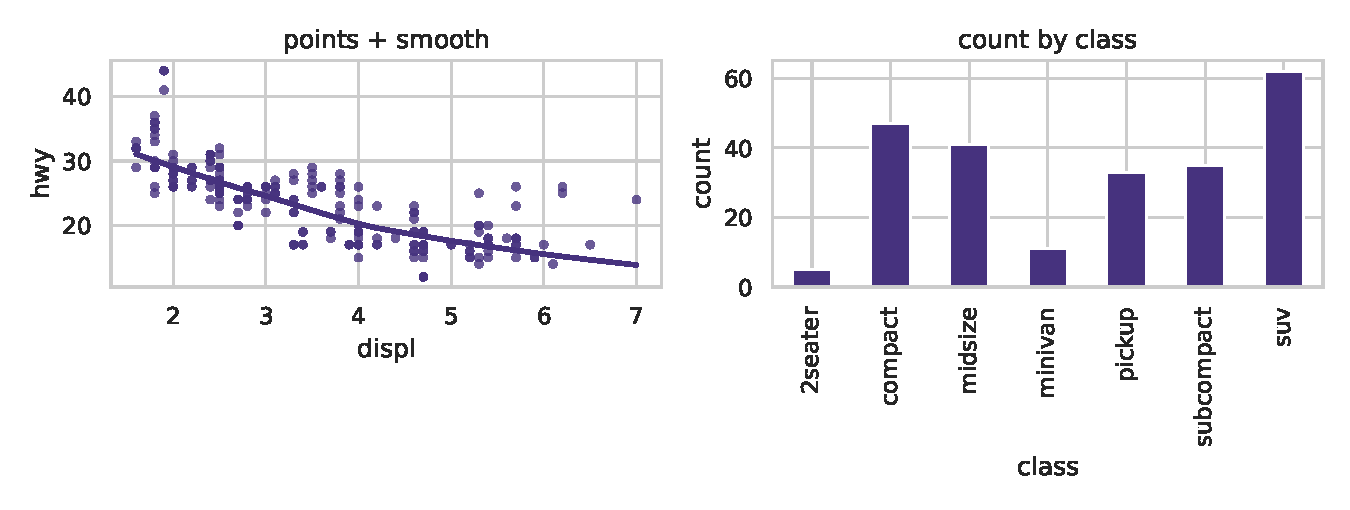
\includegraphics[width=0.95\textwidth]{figures/L03_geoms.pdf}
\caption{Left: points with a LOESS smooth. Right: the count stat behind a bar chart.}
\label{fig:L03-geoms}
\end{figure}

\subsection{The layered grammar of graphics}
\begin{definition}[Layered grammar of graphics]\label{def:L03-grammar}
Every \texttt{ggplot2} graph fits the template
\begin{center}
\begin{minipage}{0.6\textwidth}
\ttfamily
ggplot(data = <DATA>) +\\
\quad <GEOM\_FUNCTION>(\\
\quad\quad mapping = aes(<MAPPINGS>),\\
\quad\quad stat = <STAT>,\\
\quad\quad position = <POSITION>\\
\quad ) +\\
\quad <COORDINATE\_FUNCTION> +\\
\quad <FACET\_FUNCTION>
\end{minipage}
\end{center}
The seven parameters (data, geom, mapping, stat, position, coordinates, facets) are enough to
describe almost any plot.
\end{definition}
The instructor's summary annotation lists what the week covered: scatter plots, viridis colours,
bar charts, facets, geoms and coordinate systems. The recap at the start of Week~2 calls
the grammar the ``key tool in data visualisation''.

\subsection{Computation}
\begin{center}
\small\begin{tabular}{@{}>{\raggedright\arraybackslash}p{7.3cm}>{\raggedright\arraybackslash}p{8.3cm}@{}}\hline
R & Python\\\hline
\texttt{geom\_smooth()} (LOESS) & \texttt{sns.regplot(..., lowess=True)} or \texttt{statsmodels.nonparametric.lowess}\\
\texttt{filter(mpg, drv=="4")} & \texttt{mpg[mpg.drv == "4"]}\\
\texttt{geom\_bar(aes(class))} & \texttt{sns.countplot(data=mpg, x="class")}\\
\texttt{stat\_summary(fun=median, ...)} & \texttt{mpg.groupby("class").hwy} \texttt{.agg(["min", "median", "max"])}\\
\texttt{fill=trans, position="dodge"} & \texttt{sns.countplot(..., hue="trans")}\\
\texttt{coord\_flip()} & \texttt{sns.countplot(..., y="class")}\\
\texttt{coord\_polar()} & \texttt{plt.subplot(projection="polar")} with \texttt{ax.bar}\\\hline
\end{tabular}
\end{center}
See \nb{week01/L03\_ggplot\_geoms.ipynb}.

\subsection{Summary}
\begin{itemize}
  \item A geom is the object that represents data. A stat is the transformation applied first.
  \item Mappings in \texttt{ggplot()} are global; mappings in a geom are local. Each layer may use its own data.
  \item \texttt{geom\_bar} $=$ \texttt{stat\_count} $+$ bars. \texttt{stat\_summary} draws min/median/max summaries.
  \item \texttt{position="dodge"}, \texttt{coord\_flip()} and \texttt{coord\_polar()} change the layout.
  \item The template has seven parameters: data, geom, mapping, stat, position, coordinates, facets.
\end{itemize}

\subsection{Exercises}
\begin{problem}\label{prob:L03-1}
Which stat does \texttt{geom\_histogram} use, and what does it compute? How is it related to \texttt{stat\_count}?
\end{problem}
\begin{problem}\label{prob:L03-2}
Reproduce the \texttt{stat\_summary} table of \cref{ex:L03-summary} for \texttt{cty} instead of \texttt{hwy}. Which class has the largest range?
\end{problem}
\begin{problem}\label{prob:L03-3}
Explain why \texttt{geom\_smooth(method = "lm")} gives a straight line while the default gives a curve. What quantity does the \texttt{lm} line minimise?
\end{problem}
\begin{problem}\label{prob:L03-4}
Make a dodged bar chart of \texttt{drv} within each \texttt{class} in Python. Which class contains all three drive types?
\end{problem}

\subsection{Further reading}
Wickham \& Grolemund, \emph{R for Data Science}, Chapter~3 (Sections on geometric objects,
statistical transformations, position adjustments, coordinate systems and the layered grammar).


\section*{Solutions to the Exercises of Chapter~\ref{ch:week01}}
\addcontentsline{toc}{section}{Solutions to the exercises}

\paragraph{\Cref{prob:L01-1}.}
$n=7$ and $\sum x_i=42$, so $\bar x=6$. The median is $x_{(4)}=5$ and the mode is $4$.
$\sum x_i^2=312$, so $\sum(x_i-\bar x)^2=312-7\cdot 36=60$ and $s^2=60/6=10$.
Quartiles (position $1+6q$): $Q_1$ is at position $2.5$, i.e.\ $(4+4)/2=4$; $Q_3$ is at position
$5.5$, i.e.\ $(7+9)/2=8$. So $\mathrm{IQR}=4$.

\paragraph{\Cref{prob:L01-2}.}
$\sum(x_i-\bar x)^2=\sum x_i^2-2\bar x\sum x_i+n\bar x^2=\sum x_i^2-2n\bar x^2+n\bar x^2=\sum x_i^2-n\bar x^2$.

\paragraph{\Cref{prob:L01-3}.}
$\bar y=\frac1n\sum(a+bx_i)=a+b\bar x$. Then $y_i-\bar y=b(x_i-\bar x)$, so $s_y^2=b^2s_x^2$ and
$s_y=\abs{b}s_x$. The map $x\mapsto a+bx$ is monotone. For $b>0$ it keeps the order, so every
quantile transforms as $q_y=a+bq_x$. For $b<0$ it reverses the order, so $Q_1^{(y)}=a+bQ_3^{(x)}$ and
$Q_3^{(y)}=a+bQ_1^{(x)}$. The positions $1+(n-1)q$ and $1+(n-1)(1-q)$ are symmetric, so this holds
exactly for R's type-7 rule. In both cases $\mathrm{IQR}_y=\abs{b}\,\mathrm{IQR}_x$.
The shift $a$ affects only the centre.

\paragraph{\Cref{prob:L01-4}.}
\texttt{aq.groupby("Month").Temp.mean()} gives $65.55$ (May), $79.10$ (June), $83.90$ (July),
$83.97$ (August) and $76.90$ (September). August is marginally the hottest month.

\paragraph{\Cref{prob:L01-5}.}
Take eight $0$'s and two $10$'s. Then $\bar x=2$, $\sigma_n^2=(8\cdot 4+2\cdot 64)/10=16$ and
$\sigma_n=4$. The two $10$'s are at distance $8=2\sigma_n$, so only $80\%$ of the data lie strictly
within $2\sigma_n$. The proportion at distance $\ge 2\sigma_n$ is $0.2\le 1/2^2=0.25$, as
Chebyshev requires.

\paragraph{\Cref{prob:L02-1}.}
Inside \texttt{aes()}, \texttt{"blue"} is treated as a (constant) variable. ggplot maps its one
level to the first default colour and adds a legend entry ``blue''. To colour every point blue,
set the colour outside \texttt{aes()}:
\texttt{geom\_point(aes(displ, hwy), colour = "blue")}.

\paragraph{\Cref{prob:L02-2}.}
A continuous variable gets a \emph{continuous} scale. The legend is a colour bar (a gradient),
not a list of discrete keys. In seaborn, \texttt{hue="cty"} with a numeric column likewise uses a
sequential palette and shows a few representative values.

\paragraph{\Cref{prob:L02-3}.}
The cross-tabulation of \texttt{drv} against \texttt{cyl} has zeros in three cells: four-wheel
drive with $5$ cylinders, and rear-wheel drive with $4$ or $5$ cylinders. All $5$-cylinder cars
are front-wheel drive, and all rear-wheel-drive cars have $6$ or $8$ cylinders.

\paragraph{\Cref{prob:L02-4}.}
\texttt{class} has $7$ levels, \texttt{drv} has $3$ and \texttt{cyl} has $4$ ($4,5,6,8$). The grid
therefore has $3\times 4=12$ panels, three of them empty (\cref{prob:L02-3}).

\paragraph{\Cref{prob:L03-1}.}
\texttt{geom\_histogram} uses \texttt{stat\_bin}. It divides the range of the continuous $x$
variable into intervals (bins) and counts the observations in each bin. \texttt{stat\_count} counts
observations at each \emph{distinct value} of a discrete variable. \texttt{stat\_bin} is its
analogue for continuous data, where the ``values'' are the bins.

\paragraph{\Cref{prob:L03-2}.}
For \texttt{cty} (min/median/max): 2seater $15/15/16$, compact $15/20/33$, midsize $15/18/23$,
minivan $11/16/18$, pickup $9/13/17$, subcompact $14/19/35$, suv $9/13/20$. The largest range is
for subcompacts: $35-14=21$.

\paragraph{\Cref{prob:L03-3}.}
\texttt{method="lm"} fits a single global linear model $y=a+bx$ by least squares. That is, it
minimises $\sum_i (y_i-a-bx_i)^2$ over $(a,b)$ (\cref{sec:L05}). The result is necessarily a
straight line. The default LOESS fits a separate weighted least-squares polynomial near each
$x_0$, so the curve can bend.

\paragraph{\Cref{prob:L03-4}.}
\texttt{sns.countplot(data=mpg, x="class", hue="drv")}. From the cross-tabulation, only
\texttt{subcompact} contains all three drive types ($4$: 4 cars, f: 22, r: 9).

% ============================================================
% Week 2 -- Introduction to linear models (exploratory)
% ============================================================
\chapter{Linear Models: First Look}\label{ch:week02}

This chapter covers Week~2 (Lectures 4--7). The instructor introduces linear models
\emph{exploratorily}, with real and simulated data and R's \texttt{lm}. The formal theory of
estimation starts in \cref{ch:week03}. Week~2 of the official syllabus is ``working with R''.
Here the Python equivalents of every R command are given alongside.

% ============================================================
% Lecture 4 -- Introduction to Linear Models
% ============================================================
\section{Introduction to Linear Models}\label{sec:L04}

\lectureheader{4}{TPJmhTmm4h0}{Week-2 slides \texttt{Feb2.pdf} (recap and ``Model: Aims and Methods'', heights data), with the instructor's handwritten annotations}

\begin{guiding*}
By the end of this lecture you should be able to:
\begin{itemize}
  \item state the aim of modelling: to find a low-dimensional summary of the relationship between a response $y$ and an explanatory variable $x$;
  \item explain ``all models are wrong but some are useful'' with an example;
  \item describe the heights data and use a jittered scatter plot;
  \item explain the training / validation / test split used to judge models.
\end{itemize}
\end{guiding*}

\subsection{Recap}
Week~1 introduced the layered grammar of graphics: scatter plots, smooth lines, bar charts,
polar coordinates and faceting. The instructor calls it the key tool in data visualisation.
Week~2 turns from \emph{looking} at data to \emph{modelling} it. The slides warn that there is
no statistical analysis yet: this week introduces the linear model exploratorily, to see
\emph{how it works}. The formal theory starts in Week~3 (\cref{sec:L08}).

\begin{note}[Practical instruction from the slides]
Download the data sets and the Week-2 R code from the course web page and keep them in the same
directory, set as R's working directory. The Python notebooks follow the same idea. All data
sets are in the project's \texttt{data/} folder, and the notebooks find it by a relative path.
\end{note}

\subsection{Aims of modelling}
\begin{definition}[Response and explanatory variable]\label{def:L04-vars}
We observe pairs $\{(x_i,y_i):1\le i\le n\}$. The variable $x$ is the
\vocab{independent} (explanatory) variable and $y$ the \vocab{dependent} (response)
variable. A \vocab{model} is a low-dimensional summary of the data set that captures the
patterns in the data, and in particular the way $y$ depends on $x$. It can then be used for
\emph{prediction}: given a new $x$, what $y$ should we expect?
\end{definition}

\begin{note}[Caution: all models are wrong, but some are useful]
The slides quote G.\,E.\,P.~Box's aphorism. The instructor's example is the ideal gas law
$PV=RT$. No real gas satisfies it exactly, yet it is a good approximation, and it helps us
\emph{understand the system}. A linear model is judged the same way: not by being true, but by
being a good enough approximation to be useful.
\end{note}

In practice, the slides list the questions one asks:
\begin{itemize}
  \item What hypotheses do we want to test with the data?
  \item How do we judge which model works better? One common method is to split the data into three parts: about $60\%$ for \vocab{training} (fitting the models), $20\%$ for \vocab{query} or validation (choosing between models), and $20\%$ for \vocab{testing} (evaluating the chosen model's performance on data it has never seen).
\end{itemize}

\subsection{The heights data}
\begin{example}[Pearson's mothers and daughters]\label{ex:L04-heights}
Between 1893 and 1898, Karl Pearson (the slides write E.\,S.~Pearson) and his colleagues collected
the heights of mothers and their adult daughters in Britain. The version used in the course
(\texttt{heights.txt}; \texttt{Heights} in the R package \texttt{alr4}) has $n=1375$ pairs. The
annotations mention ``about 1500 odd'' and the restriction to daughters aged at least $18$
and mothers under $65$.
\begin{itemize}
  \item \texttt{Mheight}: height of the mother (inches), mean $62.45$;
  \item \texttt{Dheight}: height of one adult daughter (inches), mean $63.75$.
\end{itemize}
The \emph{object of study} is the question: \emph{how does the daughter's height depend on the
height of the mother?}
\end{example}

Heights were rounded to the nearest inch in the original records, so many points coincide. A
\vocab{jitter plot} moves each data point by a small uniformly distributed amount, here
$U(-0.5,0.5)$ in each coordinate, so that overlapping points become visible.

\begin{figure}[ht]
\centering
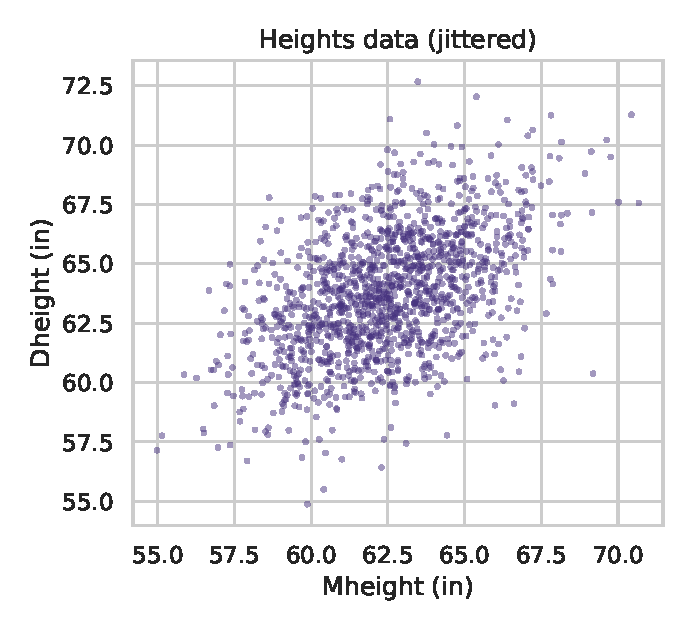
\includegraphics[width=0.5\textwidth]{figures/L04_heights.pdf}
\caption{Jittered scatter plot of daughter's height against mother's height.}
\label{fig:L04-heights}
\end{figure}

The instructor then restricts attention to the middle of the plot: mothers between about $58$
and $68$ inches. His annotations point out two features. There are \emph{no unusually tall
daughters of short mothers}, and \emph{no short daughters of very tall mothers}. The scatter
drifts upwards: taller mothers tend to have taller daughters. The plan is to develop a
technique that fits a linear model to the data $\{(x_i,y_i)\}$, that is, to find $a_1,a_2$ such
that
\[
y = a_1 + a_2 x
\]
is a good approximation. The technique is least squares. It is built step by step in
\cref{sec:L05}. It can also identify outliers: points far from the fitted line.

\begin{note}[Supplementary: the fitted line and ``regression to the mean'']
Anticipating \cref{sec:L05}, the least-squares line for these data is
\[
\widehat{\text{Dheight}} = 29.917 + 0.542\,\text{Mheight}, \qquad R^2 = 0.241.
\]
The slope $0.54<1$ means that a mother who is $1$ inch taller than average has a daughter who is
on average only about half an inch taller than average. This is Galton's \emph{regression to the
mean}. The word ``regression'' comes from this phenomenon. $R^2$ is defined in \cref{sec:L17}.
Only about a quarter of the variation in daughters' heights is explained by mothers' heights.
\end{note}

\begin{figure}[ht]
\centering
\begin{tikzpicture}[>=stealth]
\draw[->] (0,0) -- (7,0) node[right] {$x$};
\draw[->] (0,0) -- (0,4.2) node[above] {$y$};
\foreach \x/\y in {0.8/1.4,1.3/1.1,1.8/2.0,2.4/1.7,3.0/2.6,3.5/2.2,4.1/3.1,4.6/2.8,5.2/3.6,5.8/3.3,6.3/3.9}
  \fill (\x,\y) circle (1.5pt);
\draw[thick,red] (0.4,1.0) -- (6.6,3.9) node[right] {$y=a_1+a_2x$};
\draw[blue,dashed] (3.5,2.2) -- (3.5,2.38);
\draw[blue,dashed] (4.1,3.1) -- (4.1,2.66);
\node[blue,font=\small] at (4.9,1.4) {residual $=y_i-(a_1+a_2x_i)$};
\draw[blue,->] (4.5,1.6) -- (4.12,2.8);
\end{tikzpicture}
\caption{The goal: a line $y=a_1+a_2x$ that summarises the cloud of points. The vertical gaps
are the residuals studied in \cref{sec:L05,sec:L06}.}
\label{fig:L04-line}
\end{figure}

\subsection{Computation}
The R code reads \texttt{heights.txt} and plots \texttt{Dheight} against \texttt{Mheight}, with
jitter. In Python:
\codeline{h = pd.read\_csv(DATA / "Heights.csv"); plt.scatter(h.mheight + rng.uniform(-.5,.5,len(h)), h.dheight + rng.uniform(-.5,.5,len(h)))}
The notebook \nb{week02/L04\_intro\_linear\_models.ipynb} also demonstrates a 60/20/20 split.

\subsection{Summary}
\begin{itemize}
  \item A model is a low-dimensional summary of how the response $y$ depends on $x$. It is used for understanding and prediction.
  \item All models are wrong, but some are useful ($PV=RT$).
  \item Heights data: $1375$ mother--daughter pairs. Jittering reveals overlapping points. Taller mothers tend to have taller daughters.
  \item Goal: find $a_1,a_2$ so that $y\approx a_1+a_2x$. Models are compared using training/validation/test splits.
\end{itemize}

\subsection{Exercises}
\begin{problem}\label{prob:L04-1}
Why does jittering by $U(-0.5,0.5)$ not change any conclusion drawn from the plot, while it would change a fitted line if we fitted to the jittered data? By how much can the mean of the jittered $x$'s differ from the true mean in expectation?
\end{problem}
\begin{problem}\label{prob:L04-2}
Split the heights data at random into $60/20/20$ parts (with a fixed seed). Fit the line to the training part and compute the mean squared prediction error on the test part.
\end{problem}
\begin{problem}\label{prob:L04-3}
Give another physical law (like $PV=RT$) that is ``wrong but useful'', and say in what regime it fails.
\end{problem}
\begin{problem}\label{prob:L04-4}
Suppose daughters' heights were \emph{exactly} equal to their mothers'. What would the scatter plot look like, and what would $a_1,a_2$ be?
\end{problem}

\subsection{Further reading}
Weisberg, \emph{Applied Linear Regression} (4th ed.), Chapter~1 (Scatterplots and Regression),
which is the source of the heights, Forbes, bass and snowfall examples. Wickham \& Grolemund,
\emph{R for Data Science}, ``Model basics''. Christensen, Chapter~6 (Regression analysis) for
the formal treatment.

% ============================================================
% Lecture 5 -- Basics of Linear Models
% ============================================================
\section{Basics of Linear Models}\label{sec:L05}

\lectureheader{5}{Ec94oyf3bKw}{Week-2 slides \texttt{Feb2.pdf} (``Linear Models'' slides on the \texttt{sim1} data), with annotations; Week-2 R code}

\begin{guiding*}
By the end of this lecture you should be able to:
\begin{itemize}
  \item describe a family of linear models $y=a_1+a_2x$ and the residuals of each member;
  \item explain why the \emph{sum of squared} residuals is the criterion used to choose the best line;
  \item find the best line numerically (\texttt{optim}) and with \texttt{lm};
  \item derive the least-squares estimates $\hat a_2=S_{xy}/S_{xx}$, $\hat a_1=\bar y-\hat a_2\bar x$.
\end{itemize}
\end{guiding*}

\subsection{Recap and motivation}
In \cref{sec:L04} we set ourselves the goal of finding $a_1,a_2$ such that $y\approx a_1+a_2x$.
To see how this works, the instructor uses a simulated data set in which we know there is a
linear pattern: \texttt{sim1}, from the R package \texttt{modelr}.

\subsection{A family of lines}
\begin{example}[The \texttt{sim1} data]\label{ex:L05-sim1}
\texttt{sim1} has $n=30$ points: three $y$-values at each of $x=1,2,\dots,10$. The scatter plot
shows a clear pattern: a linear relationship. To explore possible models, the instructor
generates $250$ lines $y=a_1+a_2x$, with the intercept $a_1$ chosen uniformly from $[-20,40]$ and
the slope $a_2$ uniformly from $[-5,5]$, and plots all $250$ lines on top of the data
(\cref{fig:L05-sim1}, left). Most of them are terrible. A few pass through the cloud of points.
\end{example}

To say which lines are good, we need a number that measures how far a line is from the data.
\begin{definition}[Residual]\label{def:L05-residual}
For the model $y=a_1+a_2x$ and the data point $(x_i,y_i)$, the \vocab{residual} is
\[
e_i(a_1,a_2)=y_i-(a_1+a_2x_i),
\]
the vertical distance (with sign) between the data point and the line. It is the part of $y_i$
that the model does not explain.
\end{definition}

The slides then choose one line from the $250$ (line number $130$), plot it, and draw the
residuals as vertical segments from each point to the line. A good line should make the
residuals small \emph{overall}. The instructor's annotation lists candidate criteria:
\begin{enumerate}
  \item minimise the sum of distances $\sum_i \abs{e_i}$ (``hard'', since $\abs{\cdot}$ is not differentiable);
  \item minimise the sum of squared distances $\sum_i e_i^2$: the \vocab{least squares} criterion (ticked on the slide).
\end{enumerate}

\begin{definition}[Least squares line]\label{def:L05-LS}
For data $\{(x_i,y_i)\}_{i=1}^n$ let
\[
f(a_1,a_2)=\sum_{i=1}^n \bigl(y_i-a_1-a_2x_i\bigr)^2 .
\]
A pair $(\hat a_1,\hat a_2)$ minimising $f$ gives the \vocab{least squares line}
$y=\hat a_1+\hat a_2 x$.
\end{definition}

\subsection{Finding the best line numerically}
The R code on the slides defines the model and a distance, then minimises the distance with a
general-purpose optimiser:
\begin{center}
\begin{minipage}{0.8\textwidth}\small\ttfamily
model1 <- function(a, data) \{ a[1] + data\$x * a[2] \}\\
measure\_distance <- function(mod, data) \{\\
\quad diff <- data\$y - model1(mod, data)\\
\quad sqrt(mean(diff\textasciicircum 2)) \}\\
best <- optim(c(0, 0), measure\_distance, data = sim1)\\
best\$par \qquad\qquad \# 4.222248 2.051204\\
measure\_distance(best\$par, sim1) \# 2.128181
\end{minipage}
\end{center}
The distance used is the \vocab{root mean squared error}
$\mathrm{RMSE}(a_1,a_2)=\sqrt{\tfrac1n\sum_i e_i(a_1,a_2)^2}=\sqrt{f(a_1,a_2)/n}$. The map
$t\mapsto\sqrt{t/n}$ is strictly increasing, so minimising RMSE is the same as minimising $f$.
\texttt{optim} (Nelder--Mead) returns intercept $4.222248$ and slope $2.051204$, with
RMSE $2.128181$. The slide plots this line: intercept $\approx 4.22$, slope $\approx 2.05$. It
seems to give a good approximation.

The slide then asks: \emph{how do we judge the model, and is this the best possible solution?}
The ``to do'' written on the slide is to minimise $f(a_1,a_2)$ exactly. R's built-in function
\texttt{lm(y \textasciitilde\ x, data = sim1)} does this and returns
\[
\hat a_1 = 4.220822,\qquad \hat a_2=2.051533 .
\]
The small difference from \texttt{optim} is numerical: Nelder--Mead stops once further progress
falls below its tolerance. \texttt{lm} solves the problem exactly, as we now show.

\subsection{The least-squares estimates}
\begin{theorem}[Least squares for a straight line]\label{thm:L05-slr}
Let $n\ge 2$ and suppose the $x_i$ are not all equal. Write
\[
\bar x=\tfrac1n\sum x_i,\quad \bar y=\tfrac1n\sum y_i,\quad
S_{xx}=\sum_{i}(x_i-\bar x)^2,\quad S_{xy}=\sum_i (x_i-\bar x)(y_i-\bar y).
\]
Then $f(a_1,a_2)=\sum(y_i-a_1-a_2x_i)^2$ has a unique minimiser
\[
\hat a_2=\frac{S_{xy}}{S_{xx}},\qquad \hat a_1=\bar y-\hat a_2\,\bar x ,
\]
and the minimum value is $f(\hat a_1,\hat a_2)=S_{yy}-S_{xy}^2/S_{xx}$, where $S_{yy}=\sum(y_i-\bar y)^2$.
\end{theorem}
\begin{proof}
We complete the square twice, so that no calculus is needed. For fixed $a_2$ write
$z_i=y_i-a_2x_i$. Then $f=\sum_i(z_i-a_1)^2$. By \cref{prop:L01-bestconst},
\[
\sum_i (z_i-a_1)^2=\sum_i (z_i-\bar z)^2+n(\bar z-a_1)^2,\qquad \bar z=\bar y-a_2\bar x .
\]
Now $z_i-\bar z=(y_i-\bar y)-a_2(x_i-\bar x)$, so
\[
\sum_i (z_i-\bar z)^2=S_{yy}-2a_2S_{xy}+a_2^2S_{xx}
= S_{xx}\Bigl(a_2-\frac{S_{xy}}{S_{xx}}\Bigr)^2 + S_{yy}-\frac{S_{xy}^2}{S_{xx}} ,
\]
where we used $S_{xx}>0$ (the $x_i$ are not all equal). Altogether
\[
f(a_1,a_2)= S_{yy}-\frac{S_{xy}^2}{S_{xx}} + S_{xx}\Bigl(a_2-\frac{S_{xy}}{S_{xx}}\Bigr)^2 + n\bigl(\bar y-a_2\bar x-a_1\bigr)^2 .
\]
The last two terms are non-negative. Both vanish if and only if $a_2=S_{xy}/S_{xx}$ and
$a_1=\bar y-a_2\bar x$. Hence this pair is the unique minimiser, and the minimum is
$S_{yy}-S_{xy}^2/S_{xx}$.
\end{proof}

\begin{corollary}\label{cor:L05-props}
The least-squares line passes through $(\bar x,\bar y)$. The residuals
$\hat e_i=y_i-\hat a_1-\hat a_2x_i$ satisfy $\sum_i\hat e_i=0$ and $\sum_i x_i\hat e_i=0$.
\end{corollary}
\begin{proof}
At $x=\bar x$ the line gives $\hat a_1+\hat a_2\bar x=\bar y$. Next,
$\hat e_i=(y_i-\bar y)-\hat a_2(x_i-\bar x)$. Summing gives $0-0=0$. Also
$\sum_i (x_i-\bar x)\hat e_i=S_{xy}-\hat a_2S_{xx}=0$. Since $\sum\hat e_i=0$, it follows that
$\sum x_i\hat e_i=\sum(x_i-\bar x)\hat e_i+\bar x\sum\hat e_i=0$.
\end{proof}
The two identities $\sum\hat e_i=0$ and $\sum x_i\hat e_i=0$ are exactly the \emph{normal
equations} of \cref{sec:L12}, written out for a straight line.

\begin{example}[A least-squares line by hand]\label{ex:L05-hand}
Take $n=4$ points with $x=(1,2,3,4)$ and $y=(2,3,5,6)$.
\begin{itemize}
  \item $\bar x=2.5$ and $\bar y=16/4=4$.
  \item Deviations: $x_i-\bar x=(-1.5,-0.5,0.5,1.5)$ and $y_i-\bar y=(-2,-1,1,2)$.
  \item $S_{xx}=2.25+0.25+0.25+2.25=5$ and $S_{xy}=3+0.5+0.5+3=7$. Also $S_{yy}=4+1+1+4=10$.
  \item $\hat a_2=7/5=1.4$ and $\hat a_1=4-1.4\times 2.5=0.5$.
  \item Fitted values: $0.5+1.4x=(1.9,3.3,4.7,6.1)$. Residuals: $(0.1,-0.3,0.3,-0.1)$. They sum to $0$, and $\sum x_i\hat e_i=0.1-0.6+0.9-0.4=0$.
  \item Minimum: $f=0.01+0.09+0.09+0.01=0.2$, which agrees with $S_{yy}-S_{xy}^2/S_{xx}=10-49/5=0.2$. The RMSE is $\sqrt{0.2/4}=0.2236$.
\end{itemize}
\end{example}

\begin{figure}[ht]
\centering
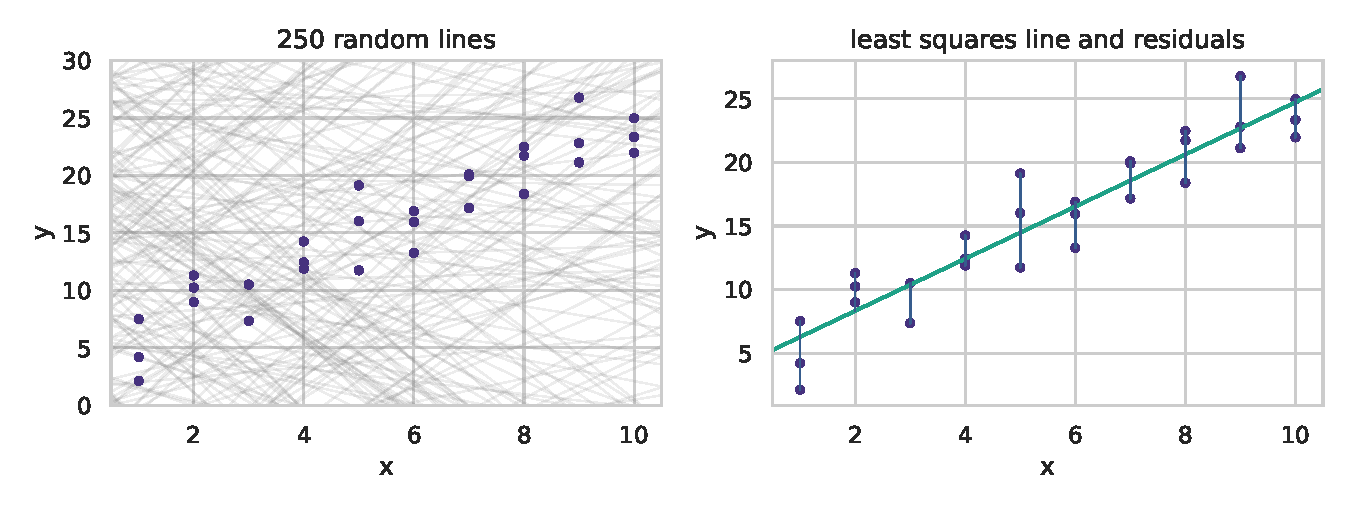
\includegraphics[width=0.95\textwidth]{figures/L05_sim1.pdf}
\caption{Left: $250$ random lines over the \texttt{sim1} data. Right: the least-squares line and its residuals.}
\label{fig:L05-sim1}
\end{figure}

\begin{note}[Supplementary: why squares?]
Squares make $f$ a smooth, convex quadratic, so the minimiser has the closed form of
\cref{thm:L05-slr}. The absolute-value criterion has no closed form and may have many
minimisers. Squares also lead to the Pythagorean geometry of \cref{sec:L12,sec:L14}. Under
normal errors, least squares coincides with maximum likelihood, and the Gauss--Markov theorem
(Week~6) shows that it is optimal among linear unbiased estimators. The price is sensitivity to
outliers: one large residual counts quadratically.
\end{note}

\subsection{Computation}
\begin{center}\small
\begin{tabular}{@{}>{\raggedright\arraybackslash}p{7cm}>{\raggedright\arraybackslash}p{8.4cm}@{}}\hline
R & Python\\\hline
\texttt{runif(250,-20,40)}, \texttt{runif(250,-5,5)} & \texttt{rng.uniform(-20, 40, 250)}, \texttt{rng.uniform(-5, 5, 250)}\\
\texttt{optim(c(0,0), measure\_distance, data=sim1)} & \texttt{scipy.optimize.minimize(rmse, [0,0], method="Nelder-Mead")}\\
\texttt{lm(y \textasciitilde\ x, data=sim1)} & \texttt{smf.ols("y \textasciitilde\ x", data=sim1).fit().params}\\\hline
\end{tabular}
\end{center}
The notebook \nb{week02/L05\_basics\_linear\_models.ipynb} also computes $\hat a_1,\hat a_2$ from
the formulas of \cref{thm:L05-slr} and checks them against \texttt{statsmodels}.

\subsection{Summary}
\begin{itemize}
  \item Residual $e_i=y_i-(a_1+a_2x_i)$. Criterion: minimise $f(a_1,a_2)=\sum e_i^2$ (least squares). This is equivalent to minimising RMSE.
  \item $\hat a_2=S_{xy}/S_{xx}$, $\hat a_1=\bar y-\hat a_2\bar x$, and $\min f=S_{yy}-S_{xy}^2/S_{xx}$.
  \item The fitted line passes through $(\bar x,\bar y)$, and $\sum\hat e_i=\sum x_i\hat e_i=0$.
  \item \texttt{sim1}: \texttt{lm} gives $4.220822$ and $2.051533$ (RMSE $2.128181$). \texttt{optim} agrees to about three decimals.
\end{itemize}

\subsection{Exercises}
\begin{problem}\label{prob:L05-1}
Show that $S_{xy}=\sum_i (x_i-\bar x)y_i=\sum_i x_iy_i-n\bar x\bar y$.
\end{problem}
\begin{problem}\label{prob:L05-2}
Fit the least-squares line by hand to $x=(0,1,2)$, $y=(1,1,4)$. Give the residuals and the minimum of $f$.
\end{problem}
\begin{problem}\label{prob:L05-3}
Show that if we fit the line through the origin, $y=a_2x$, the least-squares slope is $\sum x_iy_i/\sum x_i^2$.
\end{problem}
\begin{problem}\label{prob:L05-4}
What happens in \cref{thm:L05-slr} if all $x_i$ are equal? Describe the set of minimisers.
\end{problem}
\begin{problem}\label{prob:L05-5}
Minimise $\sum\abs{e_i}$ for \texttt{sim1} numerically (Nelder--Mead) and compare the line with the least-squares line.
\end{problem}

\subsection{Further reading}
Wickham \& Grolemund, \emph{R for Data Science}, ``Model basics'' (the \texttt{sim1} example).
Weisberg, \emph{ALR}, Chapter~2 (Simple linear regression). Christensen, Chapter~6.
Rao, \S4a (least squares).

% ============================================================
% Lecture 6 -- More on Linear Models - Residuals
% ============================================================
\section{More on Linear Models: Residuals}\label{sec:L06}

\lectureheader{6}{YlAdFp_3j1M}{Week-2 slides \texttt{Feb2.pdf} (``Linear Models: best line'', Forbes data, residual plots), with annotations; Week-2 R code}

\begin{guiding*}
By the end of this lecture you should be able to:
\begin{itemize}
  \item fit a least-squares line with \texttt{lm} and read off its coefficients;
  \item draw and interpret a \emph{residual plot}: residuals against the explanatory variable;
  \item recognise curvature and outliers from a residual plot;
  \item explain why a transformation (here $\log$) can make a relationship linear.
\end{itemize}
\end{guiding*}

\subsection{Recap}
In \cref{sec:L05} we defined residuals $e_i=y_i-(a_1+a_2x_i)$ and chose the line minimising
$\sum e_i^2$. For \texttt{sim1}, \texttt{lm} returned $(4.220822,\,2.051533)$. This lecture
applies the method to real data. It also shows that the residuals left over after fitting are
the main diagnostic tool: they tell us whether a straight line was the right model in the first
place.

\subsection{Forbes' boiling-point data}
\begin{example}[Forbes, 1857]\label{ex:L06-forbes}
In the 1840s and 1850s the Scottish physicist James D.~Forbes collected data in the Alps and in
Scotland. He wanted to estimate altitude from the \emph{boiling point of water}, which could
replace the fragile barometers of the time. The data set (\texttt{forbes.txt}; \texttt{Forbes}
in \texttt{alr4}) has $n=17$ pairs:
\begin{itemize}
  \item \texttt{bp} = boiling point of water ($^\circ$F), from $194.3$ to $212.2$;
  \item \texttt{pres} = atmospheric pressure (inches of mercury), from $20.79$ to $30.06$.
\end{itemize}
The slides plot \texttt{Pressure} against \texttt{Temperature} and use \texttt{lm} to find the
best line.
\end{example}

Fitting $\text{pres} = a_1 + a_2\,\text{bp}$ by least squares gives
\[
\widehat{\text{pres}}=-81.0637+0.5229\,\text{bp}.
\]
In the scatter plot the points lie very close to this line, and $R^2=0.9944$. Judged by the
scatter plot alone, the fit looks almost perfect.

\begin{definition}[Residual plot]\label{def:L06-residplot}
For a fitted line $\hat y_i=\hat a_1+\hat a_2x_i$, the \vocab{fitted residuals} are
$\hat e_i=y_i-\hat y_i$. A \vocab{residual plot} plots $\hat e_i$ against $x_i$ (or against
$\hat y_i$). If the straight-line model is adequate, the residual plot should look like a
structureless horizontal band around $0$.
\end{definition}

The residual plot for Forbes' data (\cref{fig:L06-forbes}, bottom left) tells a different story.
The instructor's annotations mark:
\begin{itemize}
  \item the \emph{largest positive residual}: case $12$ ($\text{bp}=204.6$), with $\hat e_{12}=0.650$, far above all the others;
  \item the \emph{most negative} residual: case $11$ ($\text{bp}=203.6$), with $\hat e_{11}=-0.257$;
  \item a \emph{curved} pattern in the rest. The residuals are positive at both ends (e.g.\ $0.151, 0.256$ at the lowest temperatures and $0.143, 0.166$ at the highest) and negative in the middle.
\end{itemize}
A systematic curve in the residuals means that the straight line is not the right shape. It
underestimates at the ends and overestimates in the middle. The residual plot magnifies
departures from the line that the scatter plot hides, because it removes the large linear trend.

\begin{figure}[ht]
\centering
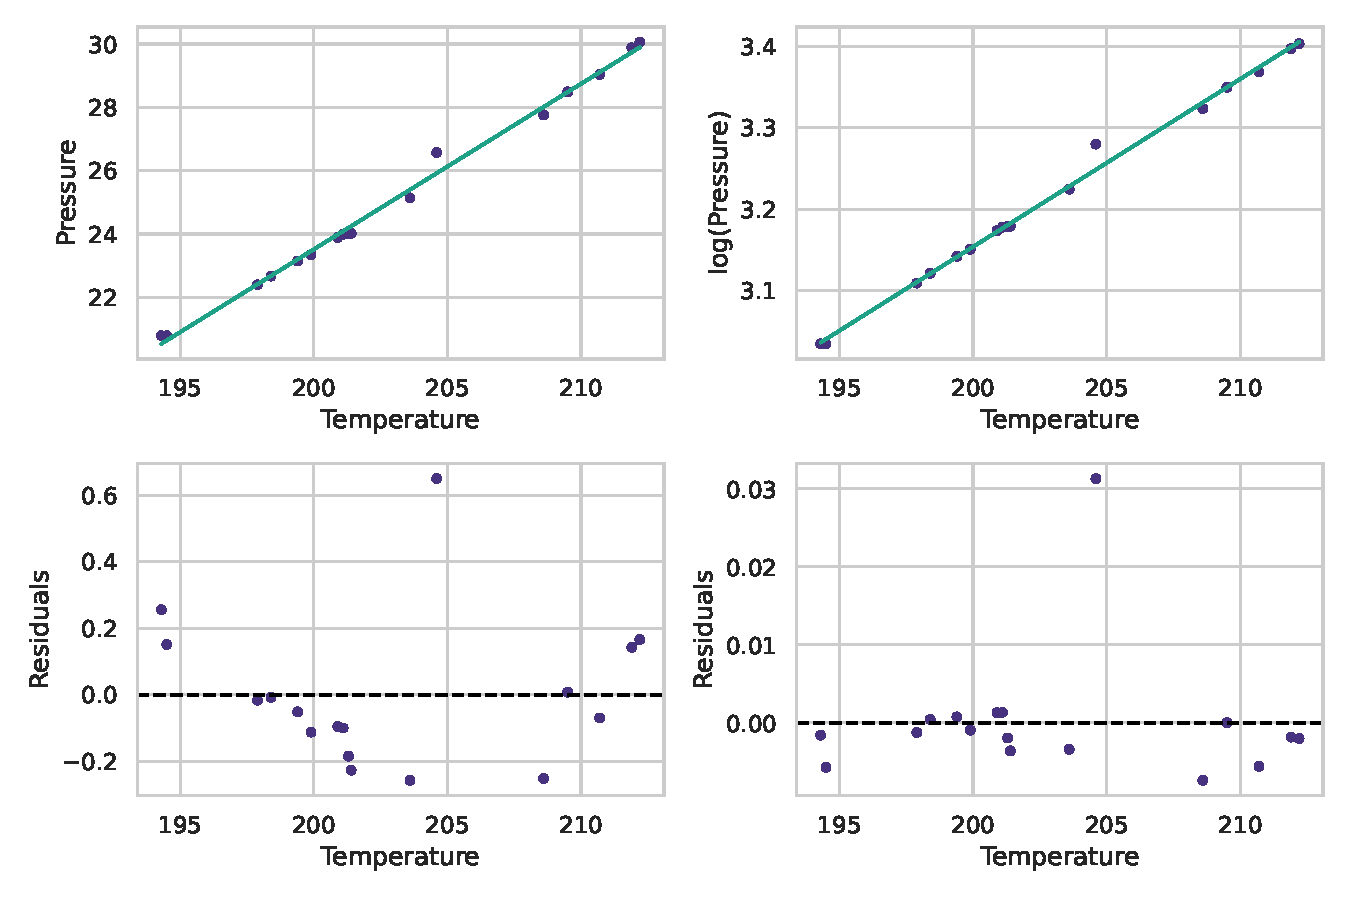
\includegraphics[width=0.9\textwidth]{figures/L06_forbes.pdf}
\caption{Forbes' data. Top: fitted lines for Pressure and for $\log$(Pressure). Bottom: the
corresponding residual plots. Curvature is visible on the left; on the right only case 12 stands out.}
\label{fig:L06-forbes}
\end{figure}

\subsection{A transformation}
The slides then note that \emph{physical theory} says that $\log(\text{Pressure})$ is linearly
related to temperature. We therefore fit
\[
\log(\text{pres}) = a_1 + a_2\,\text{bp}.
\]
With natural logarithms, least squares gives
$\widehat{\log(\text{pres})}=-0.97087+0.020622\,\text{bp}$. The \texttt{alr4} file also contains
\texttt{lpres} $=100\log_{10}(\text{pres})$, which gives $-42.138+0.8955\,\text{bp}$. The two fits
are equivalent up to the constant factor $100/\ln 10$. The residual plot (bottom right) no longer
shows curvature: apart from case~12, the residuals form a horizontal band. Case~12, with residual
$0.0313$ on the log scale, is now clearly an \emph{outlier}. It could be a recording error.

\begin{note}[Supplementary: the physics behind the log]
The Clausius--Clapeyron relation says that the vapour pressure $P$ of a liquid at absolute
temperature $T$ satisfies, approximately, $\log P = c - L/(RT)$. Here $L$ is the latent heat
and $R$ is the gas constant. Water boils when its vapour pressure equals the atmospheric
pressure, so $\log(\text{pres})$ is linear in $1/T$. Over the narrow range
$194$--$212\,^\circ$F (about $363$--$373$\,K), $1/T$ is itself very nearly linear in $T$. This is
why $\log(\text{pres})$ is linear in bp to high accuracy.
\end{note}

\begin{note}[Supplementary: what one outlier does]
Refitting the log model without case~12 gives $\widehat{\log(\text{pres})}=-0.95177+0.020519\,\text{bp}$,
and $R^2$ rises from $0.99496$ to $0.99957$. The slope hardly changes, so the outlier does not
distort the line much. Its main effect is to inflate the residual variance. Whether to delete an
outlier is a scientific decision, not a statistical one. It should be reported either way.
\end{note}

\begin{proposition}[Supplementary: residuals carry no linear trend]\label{prop:L06-noline}
If a least-squares line is fitted to $(x_i,y_i)$, then the least-squares line fitted to the
residual plot $(x_i,\hat e_i)$ is the horizontal line $y=0$.
\end{proposition}
\begin{proof}
By \cref{thm:L05-slr}, the slope for the data $(x_i,\hat e_i)$ is
$\sum_i (x_i-\bar x)(\hat e_i-\bar{\hat e})/S_{xx}$. By \cref{cor:L05-props},
$\bar{\hat e}=0$ and $\sum_i (x_i-\bar x)\hat e_i=0$, so the slope is $0$. The intercept is then
$\bar{\hat e}-0\cdot\bar x=0$.
\end{proof}
So any \emph{linear} tendency is removed by the fit. What remains visible in a residual plot is
non-linear structure (curvature), unequal spread, or unusual points. These are exactly the
features we look for.

\subsection{Computation}
\begin{center}\small
\begin{tabular}{@{}>{\raggedright\arraybackslash}p{7cm}>{\raggedright\arraybackslash}p{8.4cm}@{}}\hline
R & Python\\\hline
\texttt{m <- lm(pres \textasciitilde\ bp, data = forbes)} & \texttt{m = smf.ols("pres \textasciitilde\ bp", data=fb).fit()}\\
\texttt{residuals(m)} & \texttt{m.resid}\\
\texttt{plot(forbes\$bp, residuals(m))} & \texttt{plt.scatter(fb.bp, m.resid)}\\
\texttt{lm(log(pres) \textasciitilde\ bp, data = forbes)} & \texttt{smf.ols("np.log(pres) \textasciitilde\ bp", data=fb).fit()}\\\hline
\end{tabular}
\end{center}
See \nb{week02/L06\_residuals.ipynb}.

\subsection{Summary}
\begin{itemize}
  \item Residual plot: $\hat e_i$ against $x_i$. It should be a structureless band around $0$.
  \item Forbes: $\widehat{\text{pres}}=-81.06+0.523\,\text{bp}$. The residuals are curved, case 12 has the largest positive residual ($0.650$) and case 11 the most negative ($-0.257$).
  \item $\log(\text{pres})$ is linear in bp (physical theory). After transforming, only the outlier (case 12) remains.
  \item The fitted residuals have zero mean and zero correlation with $x$, so only non-linear structure can show up.
\end{itemize}

\subsection{Exercises}
\begin{problem}\label{prob:L06-1}
Show that $\sum_i \hat y_i\hat e_i=0$ for a least-squares line. Deduce that plotting residuals against fitted values also shows no linear trend.
\end{problem}
\begin{problem}\label{prob:L06-2}
Refit Forbes' log model without case $12$ in Python and confirm the coefficients $-0.95177$ and $0.020519$.
\end{problem}
\begin{problem}\label{prob:L06-3}
Show that if $\text{lpres}=100\log_{10}(\text{pres})$, the least-squares coefficients for lpres are exactly $100/\ln 10$ times those for $\ln(\text{pres})$.
\end{problem}
\begin{problem}\label{prob:L06-4}
Describe the residual plot you would expect if the spread of $y$ around the true line grew with $x$.
\end{problem}

\subsection{Further reading}
Weisberg, \emph{ALR}, Chapter~1 (Forbes' data) and Chapter~9 (outliers and diagnostics).
Christensen, Chapter~12 (Model diagnostics).

% ============================================================
% Lecture 7 -- Play with more data sets in R
% ============================================================
\section{Playing with More Data Sets}\label{sec:L07}

\lectureheader{7}{V8SQrXbSA44}{Week-2 slides \texttt{Feb2.pdf} (smallmouth bass and snowfall examples), with annotations; Week-2 data sets \texttt{wblake.txt}, \texttt{snow.txt}}

\begin{guiding*}
By the end of this lecture you should be able to:
\begin{itemize}
  \item explore a data set with a discrete explanatory variable (age) and compare the mean response at each level with a fitted line;
  \item explain why a regression of $y$ on $x$ cannot simply be inverted to predict $x$ from $y$;
  \item recognise from a scatter plot and a fitted line when two variables are essentially unrelated.
\end{itemize}
\end{guiding*}

\subsection{Recap}
We can fit a least-squares line (\cref{sec:L05}) and check it with a residual plot
(\cref{sec:L06}). The instructor now applies the same steps to further data sets from
Weisberg's book. The point is to see how scatter plots guide the choice of a model.

\subsection{Length at age for smallmouth bass}
\begin{example}[West Bearskin Lake bass]\label{ex:L07-bass}
The data (\texttt{wblake.txt}; \texttt{wblake} in \texttt{alr4}) record the \texttt{Length}
(mm) and \texttt{Age} (years) of $n=439$ smallmouth bass caught in West Bearskin Lake, Minnesota,
USA, in 1991. Age is determined from annular rings on the fish's scales, like the rings of a
tree. Ages run from $1$ to $8$, with counts
\begin{center}
\begin{tabular}{lcccccccc}\hline
Age & 1 & 2 & 3 & 4 & 5 & 6 & 7 & 8\\
number of fish & 38 & 72 & 94 & 15 & 68 & 87 & 61 & 4\\\hline
\end{tabular}
\end{center}
\end{example}

Because Age is discrete, the scatter plot consists of eight vertical strips. Within each strip
there is a spread of lengths. Fish of the same age differ in length. We can summarise each strip
by its mean length and compare the eight means with the least-squares line
\[
\widehat{\text{Length}} = 65.53 + 30.32\,\text{Age}.
\]
The means lie close to the line for young fish but bend below it for the oldest: growth slows
with age. The instructor's annotation makes a second point. The graph shows how length
depends on age, but \emph{we cannot use the line to predict age from length}. Each strip is wide,
and the strips overlap heavily. A fish of length $200$\,mm could plausibly be $3$, $4$ or $5$
years old. Moreover, inverting the line $y=a_1+a_2x$ is not the same as regressing $x$ on $y$.

\begin{proposition}[Supplementary: regression is not symmetric]\label{prop:L07-asym}
Let $\hat a_2^{(y|x)}=S_{xy}/S_{xx}$ be the least-squares slope of $y$ on $x$ and
$\hat b_2^{(x|y)}=S_{xy}/S_{yy}$ the slope of $x$ on $y$. Then
\[
\hat a_2^{(y|x)}\cdot \hat b_2^{(x|y)}=r^2,\qquad r=\frac{S_{xy}}{\sqrt{S_{xx}S_{yy}}} .
\]
The line of $y$ on $x$, rewritten as a line for $x$ in terms of $y$, has slope $1/\hat a_2^{(y|x)}$.
This equals $\hat b_2^{(x|y)}$ only when $r^2=1$, i.e.\ when all points lie exactly on a line.
\end{proposition}
\begin{proof}
Both formulas come from \cref{thm:L05-slr}, with the roles of $x$ and $y$ swapped for the second.
Multiplying, $\hat a_2\hat b_2 = S_{xy}^2/(S_{xx}S_{yy})=r^2$. The equality
$1/\hat a_2=\hat b_2$ is equivalent to $\hat a_2\hat b_2=1$, i.e.\ to $r^2=1$. By the
Cauchy--Schwarz inequality $r^2\le 1$, with equality if and only if the vectors
$(y_i-\bar y)$ and $(x_i-\bar x)$ are proportional.
\end{proof}

\subsection{Predicting the weather: snowfall}
\begin{example}[Fort Collins snowfall]\label{ex:L07-snow}
Can the snowfall of early winter predict the snowfall of late winter? The data (\texttt{snow.txt};
\texttt{ftcollinssnow} in \texttt{alr4}) give, for $93$ years starting in 1900 at Fort Collins,
Colorado, the snowfall (inches) from September to December (\texttt{Early}) and from January to
June (\texttt{Late}).
\end{example}
The scatter plot of Late against Early is a shapeless cloud. The least-squares line is
\[
\widehat{\text{Late}} = 28.64 + 0.2035\,\text{Early},
\]
with $R^2=0.0258$ and sample correlation $r=0.161$. The slope is small and, as we will be able to
test in \cref{sec:L16}, not significantly different from $0$ (p-value $0.124$). The fitted line
is hardly distinguishable from the horizontal line at the mean of Late. The instructor's
conclusion, written on the slide: early and late snowfall are \emph{not related}.
A good-looking line can always be computed. Whether it means anything is a separate question.

\begin{figure}[ht]
\centering
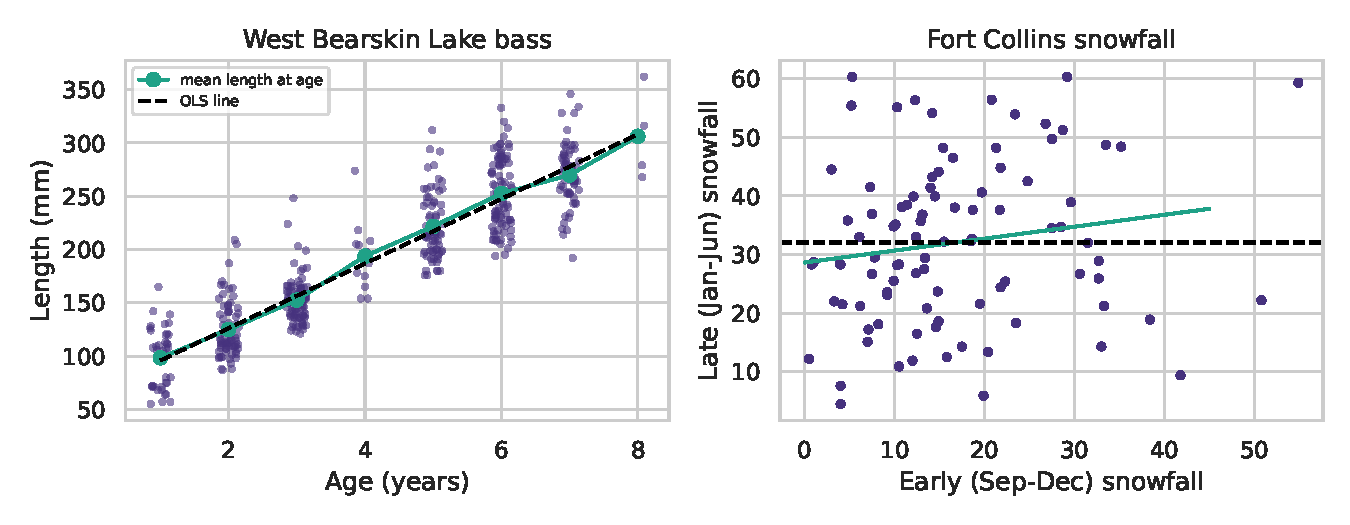
\includegraphics[width=0.95\textwidth]{figures/L07_bass_snow.pdf}
\caption{Left: bass length against age, with mean length at each age and the least-squares line.
Right: late against early snowfall; the fitted line (solid) is close to the mean of Late (dashed).}
\label{fig:L07-bass-snow}
\end{figure}

\subsection{Computation}
The Week-2 R code reads each \texttt{.txt} file, plots it and calls \texttt{lm}. In Python:
\codeline{w = pd.read\_csv(DATA / "wblake.csv"); w.groupby("Age").Length.mean(); smf.ols("Length \textasciitilde\ Age", w).fit()}
\codeline{sn = pd.read\_csv(DATA / "ftcollinssnow.csv"); smf.ols("Late \textasciitilde\ Early", sn).fit().summary()}
See \nb{week02/L07\_more\_datasets.ipynb}.

\subsection{Summary}
\begin{itemize}
  \item Bass: $\widehat{\text{Length}}=65.53+30.32\,\text{Age}$. Mean length grows with age but levels off. Age cannot be predicted reliably from length.
  \item The regressions of $y$ on $x$ and of $x$ on $y$ differ unless $r^2=1$. Their slopes multiply to $r^2$.
  \item Snowfall: slope $0.2035$, $R^2=0.026$. Early and late snowfall are essentially unrelated.
\end{itemize}

\subsection{Exercises}
\begin{problem}\label{prob:L07-1}
Compute the least-squares line of Age on Length for the bass data and compare its slope with $1/30.32$.
\end{problem}
\begin{problem}\label{prob:L07-2}
Show that $\hat a_2=r\, s_y/s_x$, where $s_x,s_y$ are the sample standard deviations.
\end{problem}
\begin{problem}\label{prob:L07-3}
For the snowfall data, compute $\sum_i(\text{Late}_i-\overline{\text{Late}})^2$ and the minimum of $f$ from \cref{thm:L05-slr}. What fraction of the total is removed by the line?
\end{problem}
\begin{problem}\label{prob:L07-4}
Fit a model in which each age has its own mean length (use \texttt{C(Age)} in the formula). Compare its residual sum of squares with that of the straight line. Which is smaller, and why must it be?
\end{problem}

\subsection{Further reading}
Weisberg, \emph{ALR}, Chapter~1 (bass and snowfall examples). Christensen, Chapter~6
(Regression) and Chapter~4 (one-way ANOVA, the ``one mean per age'' model).


\section*{Solutions to the Exercises of Chapter~\ref{ch:week02}}
\addcontentsline{toc}{section}{Solutions to the exercises}

\paragraph{\Cref{prob:L04-1}.}
Jitter only affects the picture, and each point moves by less than half an inch, so no visual
conclusion changes. A line fitted to jittered data would change slightly, because it is a
function of the data. The jitter $U_i\sim U(-0.5,0.5)$ has mean $0$, so the jittered mean
$\bar x+\bar U$ equals the true mean in expectation. Its standard deviation is
$\sqrt{1/12}/\sqrt n\approx 0.0078$ for $n=1375$.

\paragraph{\Cref{prob:L04-2}.}
With seed $2024$ (see the notebook), the training set has $825$ pairs and the test set $275$.
The training fit is $\widehat{\text{Dheight}}=32.281+0.5052\,\text{Mheight}$, and the mean
squared prediction error on the test set is $5.08$ square inches. The exact numbers depend on the
seed.

\paragraph{\Cref{prob:L04-3}.}
Newton's laws of motion: very accurate for everyday speeds, but they fail when speeds approach
the speed of light (relativity) or at atomic scales (quantum mechanics). Another example is
Hooke's law $F=-kx$, which fails for large extensions of a spring.

\paragraph{\Cref{prob:L04-4}.}
All points would lie on the line $y=x$, with no scatter, so $a_1=0$ and $a_2=1$. The real data
have slope $0.54$ and a large scatter, so heights are far from exactly inherited.

\paragraph{\Cref{prob:L05-1}.}
$\sum(x_i-\bar x)(y_i-\bar y)=\sum(x_i-\bar x)y_i-\bar y\sum(x_i-\bar x)=\sum(x_i-\bar x)y_i$,
since $\sum(x_i-\bar x)=0$. Also $\sum(x_i-\bar x)y_i=\sum x_iy_i-\bar x\sum y_i=\sum x_iy_i-n\bar x\bar y$.

\paragraph{\Cref{prob:L05-2}.}
$\bar x=1$, $\bar y=2$, $S_{xx}=2$, $S_{xy}=(-1)(-1)+0\cdot(-1)+1\cdot 2=3$, $S_{yy}=6$.
So $\hat a_2=1.5$ and $\hat a_1=2-1.5=0.5$. Fitted values $(0.5,2,3.5)$, residuals $(0.5,-1,0.5)$,
and $\min f=0.25+1+0.25=1.5=S_{yy}-S_{xy}^2/S_{xx}=6-4.5$.

\paragraph{\Cref{prob:L05-3}.}
$g(a)=\sum(y_i-ax_i)^2=\sum y_i^2-2a\sum x_iy_i+a^2\sum x_i^2$. If $\sum x_i^2>0$, complete the square:
$g(a)=\sum x_i^2\,(a-\sum x_iy_i/\sum x_i^2)^2+\text{const}$. The minimum is at $a=\sum x_iy_i/\sum x_i^2$.

\paragraph{\Cref{prob:L05-4}.}
If all $x_i=c$, then $f(a_1,a_2)=\sum(y_i-(a_1+a_2c))^2$ depends only on $t=a_1+a_2c$. It is
minimised when $t=\bar y$ (\cref{prop:L01-bestconst}). The minimisers form the whole line
$\{(a_1,a_2):a_1+a_2c=\bar y\}$, so there is no unique slope. The slope is \emph{not
identifiable} from such data. This is a first example of the non-uniqueness studied in
\cref{sec:L08,sec:L13}.

\paragraph{\Cref{prob:L05-5}.}
See the notebook. The least-absolute-deviations line is close to the least-squares line for
\texttt{sim1}, because the data have no outliers. Nelder--Mead may return slightly different
answers from different starting points, because the $L^1$ objective is flat in places.

\paragraph{\Cref{prob:L06-1}.}
$\hat y_i=\hat a_1+\hat a_2x_i$, so $\sum\hat y_i\hat e_i=\hat a_1\sum\hat e_i+\hat a_2\sum x_i\hat e_i=0$
by \cref{cor:L05-props}. Since also $\sum\hat e_i=0$, the argument of \cref{prop:L06-noline}
with $x_i$ replaced by $\hat y_i$ shows that the least-squares line through $(\hat y_i,\hat e_i)$
is $y=0$.

\paragraph{\Cref{prob:L06-2}.}
In Python, \texttt{smf.ols("np.log(pres) \textasciitilde\ bp", fb.drop(11)).fit().params} gives
$-0.951766$ and $0.020519$. Case $12$ is row $11$ in zero-based indexing.

\paragraph{\Cref{prob:L06-3}.}
$100\log_{10}p=c\ln p$ with $c=100/\ln 10$. If $(\hat a_1,\hat a_2)$ minimises
$\sum(\ln p_i-a_1-a_2x_i)^2$, then $\sum(c\ln p_i-b_1-b_2x_i)^2=c^2\sum(\ln p_i-b_1/c-(b_2/c)x_i)^2$
is minimised at $b_j=c\hat a_j$. Check: $0.020622\times 43.4294=0.8956$.

\paragraph{\Cref{prob:L06-4}.}
A ``fan'' or ``megaphone'' shape: residuals scattered narrowly around $0$ for small $x$ and
widely for large $x$. This indicates non-constant variance (heteroscedasticity), which violates
the assumption $\Var(\eps_i)=\sigma^2$ introduced in \cref{sec:L09}.

\paragraph{\Cref{prob:L07-1}.}
Age on Length gives $\widehat{\text{Age}}=-0.993+0.02693\,\text{Length}$. The slope $0.02693$ is
smaller than $1/30.32=0.03298$, as \cref{prop:L07-asym} predicts: $30.32\times0.02693=r^2=0.816$.

\paragraph{\Cref{prob:L07-2}.}
$\hat a_2=S_{xy}/S_{xx}=\dfrac{S_{xy}}{\sqrt{S_{xx}S_{yy}}}\sqrt{\dfrac{S_{yy}}{S_{xx}}}
=r\sqrt{\dfrac{S_{yy}/(n-1)}{S_{xx}/(n-1)}}=r\,s_y/s_x$.

\paragraph{\Cref{prob:L07-3}.}
$S_{yy}=17572.41$ and $\min f=17118.83$. The line removes $1-17118.83/17572.41=2.58\%$ of the
total, which is exactly $R^2$.

\paragraph{\Cref{prob:L07-4}.}
The residual sum of squares is $358595.5$ for the line and $348491.7$ for the separate-means model.
The separate-means model is smaller, and it must be. Every straight line $a_1+a_2\,\text{Age}$
assigns one fitted value to each age, so it is a special case of ``one mean per age''. Minimising
over the larger family can only give a smaller (or equal) minimum. The difference is the lack of
fit of the straight line. Testing whether it is significant uses the $F$-tests of Week~8.

% ============================================================
% Week 3 -- Least squares estimation, estimable linear functions
% ============================================================
\chapter{Linear Models and Estimability}\label{ch:week03}

This chapter covers Week~3 (Lectures 8--10): the one-way classification model, the general
linear model $(Y,X\beta,\sigma^2I_n)$, and the characterisation of estimable linear parametric
functions. From here on, the source for each lecture is the instructor's handwritten notes.
Every step the notes leave as an exercise is proved in full.

% ============================================================
% Lecture 8 -- Fundamentals of Linear Models and the estimation problem
% ============================================================
\section{Fundamentals of Linear Models and the Estimation Problem}\label{sec:L08}

\lectureheader{8}{9RbRhz776-k}{Week-3 handwritten notes \texttt{Feb9.pdf}, first part (``Model 1'', within/between variation, design matrix, identifiability)}

\begin{guiding*}
By the end of this lecture you should be able to:
\begin{itemize}
  \item write down the one-way classification model $Y_{ij}=\mu+\mu_i+\eps_{ij}$ and state the three estimation questions for it;
  \item define $\SSW$, $\SSB$ and $\TSS$, prove $\TSS=\SSW+\SSB$, and state and prove their distributions and independence;
  \item write the model as $Y=X\beta+\eps$, find $\rank(X)$, and explain why its parameters are \emph{not identifiable};
  \item show that contrasts such as $\mu_1-\mu_2$ are identifiable, and that a constraint like $\sum\mu_i=0$ makes all parameters identifiable.
\end{itemize}
\end{guiding*}

\subsection{Motivation}
Week~2 fitted lines to data. From now on we develop the \emph{theory}: when can parameters be
estimated, what is the best estimate, and how are its errors distributed? The instructor begins
with the model that underlies the analysis of variance.

\subsection{The one-way classification model}
\begin{definition}[Model 1: one-way classification]\label{def:L08-oneway}
There are $k$ populations (groups). From population $i$ we observe $n_i$ values $Y_{i1},\dots,Y_{in_i}$:
\[
Y_{ij}=\mu+\mu_i+\eps_{ij},\qquad 1\le i\le k,\quad 1\le j\le n_i,
\]
where $\mu,\mu_1,\dots,\mu_k\in\RR$ are unknown and the errors $\eps_{ij}\sim\N(0,\sigma^2)$ are
independent. The total sample size is $n=n_1+n_2+\dots+n_k$. Here $\mu$ is a general
level and $\mu_i$ the \vocab{effect} of group $i$. The mean of population $i$ is $\mu+\mu_i$.
\end{definition}
The data can be pictured as $k$ columns:
\begin{center}
\begin{tabular}{cccc}\hline
Population 1 & Population 2 & $\cdots$ & Population $k$\\\hline
$Y_{11}$ & $Y_{21}$ & & $Y_{k1}$\\
$\vdots$ & $\vdots$ & & $\vdots$\\
$Y_{1n_1}$ & $Y_{2n_2}$ & & $Y_{kn_k}$\\\hline
\end{tabular}
\end{center}

\begin{question}\label{q:L08-questions}
The lecture poses three questions.
\begin{enumerate}
  \item[(i)] Can we estimate $\mu$? If yes, what is the estimate?
  \item[(ii)] Can we estimate $\mu+\mu_i$? If yes, what is the estimate?
  \item[(iii)] Can we estimate $\mu_i-\mu_j$ for $1\le i\ne j\le k$? If yes, what is the estimate?
\end{enumerate}
\end{question}
The answers are (i) no, (ii) yes, (iii) yes. This lecture shows why (i) fails and gives
unbiased estimates for (iii). \Cref{sec:L10,sec:L13} give the general theory.

\subsection{Within-group and between-group variation}
Write $\bar Y_{i\cdot}=\frac1{n_i}\sum_{j=1}^{n_i}Y_{ij}$ for the mean of group $i$ and
$\bar Y_{\cdot\cdot}=\frac1n\sum_{i=1}^k\sum_{j=1}^{n_i}Y_{ij}$ for the grand mean.

\begin{definition}[Sums of squares]\label{def:L08-SS}
\begin{itemize}
  \item The variance of group $i$ is estimated unbiasedly by the $i$th sample variance
  $S_i^2=\frac{1}{n_i-1}\sum_{j=1}^{n_i}(Y_{ij}-\bar Y_{i\cdot})^2$ (for $n_i\ge 2$).
  \item The \vocab{sum of squares within} groups is $\SSW=\sum_{i=1}^k\sum_{j=1}^{n_i}(Y_{ij}-\bar Y_{i\cdot})^2$.
  \item The \vocab{sum of squares between} groups is $\SSB=\sum_{i=1}^k n_i(\bar Y_{i\cdot}-\bar Y_{\cdot\cdot})^2$.
  \item The \vocab{total sum of squares} is $\TSS=\sum_{i=1}^k\sum_{j=1}^{n_i}(Y_{ij}-\bar Y_{\cdot\cdot})^2$.
\end{itemize}
\end{definition}

\begin{theorem}[Decomposition of the total sum of squares]\label{thm:L08-decomp}
$\TSS=\SSW+\SSB$.
\end{theorem}
\begin{proof}
Write $Y_{ij}-\bar Y_{\cdot\cdot}=(Y_{ij}-\bar Y_{i\cdot})+(\bar Y_{i\cdot}-\bar Y_{\cdot\cdot})$ and square:
\[
\TSS=\sum_{i,j}(Y_{ij}-\bar Y_{i\cdot})^2+\sum_{i,j}(\bar Y_{i\cdot}-\bar Y_{\cdot\cdot})^2
+2\sum_{i=1}^k(\bar Y_{i\cdot}-\bar Y_{\cdot\cdot})\sum_{j=1}^{n_i}(Y_{ij}-\bar Y_{i\cdot}).
\]
The inner sum in the cross term is $\sum_j Y_{ij}-n_i\bar Y_{i\cdot}=0$ for every $i$, so the
cross term vanishes. The first sum is $\SSW$. In the second the summand does not depend on
$j$, so it equals $\sum_i n_i(\bar Y_{i\cdot}-\bar Y_{\cdot\cdot})^2=\SSB$.
\end{proof}

The notes then list distributional facts, the first two posed as exercises. To prove them we
need two tools about normal vectors.

\begin{lemma}[Quadratic forms in projections]\label{lem:L08-chisq}
Let $Z\sim\N(0,I_m)$ (i.e.\ $Z_1,\dots,Z_m$ i.i.d.\ $\N(0,1)$) and let $A$ be an $m\times m$
symmetric matrix with $A^2=A$ and $\rank(A)=r$. Then $Z\T AZ\sim\chi^2_r$.
\end{lemma}
\begin{proof}
By the spectral theorem, $A=Q\Lambda Q\T$ with $Q$ orthogonal and $\Lambda$ diagonal. From
$A^2=A$ we get $\Lambda^2=\Lambda$, so every eigenvalue is $0$ or $1$. The number of $1$'s is
$\rank(\Lambda)=\rank(A)=r$. Order them first. Put $W=Q\T Z$. $W$ is a linear function of a
normal vector, so it is normal, with mean $0$ and covariance $Q\T I Q=I$. Hence
$W_1,\dots,W_m$ are i.i.d.\ $\N(0,1)$, and
$Z\T AZ=W\T\Lambda W=W_1^2+\dots+W_r^2\sim\chi^2_r$.
\end{proof}

\begin{lemma}[Uncorrelated jointly normal vectors are independent]\label{lem:L08-indep}
If $(U,V)$ is jointly normal and $\Cov(U,V)=0$ (every component of $U$ is uncorrelated with
every component of $V$), then $U$ and $V$ are independent. Hence so are $g(U)$ and $h(V)$ for any
functions $g,h$.
\end{lemma}
\begin{proof}
Let $m_U,m_V$ be the means and $\Sigma_U,\Sigma_V$ the covariance matrices. The joint covariance
matrix is block diagonal, $\mathrm{diag}(\Sigma_U,\Sigma_V)$. The moment generating function of a
normal vector $W$ with mean $m$ and covariance $\Sigma$ is $\EE e^{t\T W}=\exp(t\T m+\tfrac12 t\T\Sigma t)$.
For $t=(s,u)$ the block structure gives
\[
\EE e^{s\T U+u\T V}=\exp\bigl(s\T m_U+\tfrac12 s\T\Sigma_Us\bigr)\exp\bigl(u\T m_V+\tfrac12 u\T\Sigma_Vu\bigr)
=\EE e^{s\T U}\,\EE e^{u\T V}.
\]
A joint moment generating function that factorises determines a product distribution, so $U\indep V$.
\end{proof}

\begin{theorem}[Distribution of the sums of squares]\label{thm:L08-dist}
In Model~1:
\begin{enumerate}
  \item $\SSW/\sigma^2\sim\chi^2_{n-k}$: $\SSW$ has $n-k$ \vocab{degrees of freedom};
  \item $\SSW$ is independent of $\SSB$;
  \item if $\mu_1=\mu_2=\dots=\mu_k$, then $\SSB/\sigma^2\sim\chi^2_{k-1}$ ($k-1$ degrees of freedom) and $\TSS/\sigma^2\sim\chi^2_{n-1}$ ($n-1$ degrees of freedom).
\end{enumerate}
\end{theorem}
\begin{proof}
(1) Fix $i$ and let $\eps_i=(\eps_{i1},\dots,\eps_{in_i})\T$. Since $Y_{ij}-\bar Y_{i\cdot}=\eps_{ij}-\bar\eps_{i\cdot}$,
\[
\sum_{j}(Y_{ij}-\bar Y_{i\cdot})^2=\eps_i\T\Bigl(I_{n_i}-\tfrac1{n_i}\one\one\T\Bigr)\eps_i .
\]
The matrix $C_i=I-\frac1{n_i}\one\one\T$ is symmetric and idempotent: $C_i^2=I-\frac2{n_i}\one\one\T+\frac1{n_i^2}\one(\one\T\one)\one\T=C_i$.
Its rank equals its trace, $n_i-1$. The trace equals the rank for idempotent matrices, because
the eigenvalues are $0$ or $1$. Applying \cref{lem:L08-chisq} to $Z=\eps_i/\sigma$ gives
$\sum_j(Y_{ij}-\bar Y_{i\cdot})^2/\sigma^2\sim\chi^2_{n_i-1}$. The $k$ groups are independent. A sum
of independent $\chi^2$ variables is $\chi^2$ with the degrees of freedom added: multiply the
moment generating functions $(1-2t)^{-(n_i-1)/2}$. So $\SSW/\sigma^2\sim\chi^2_{\sum(n_i-1)}=\chi^2_{n-k}$.

(2) $\SSW$ is a function of the vector $U=(\eps_{ij}-\bar\eps_{i\cdot})_{i,j}$. $\SSB$ is a function of
$V=(\bar Y_{1\cdot},\dots,\bar Y_{k\cdot})$, because $\bar Y_{\cdot\cdot}=\frac1n\sum n_i\bar Y_{i\cdot}$. Both are linear
functions of the normal vector $\eps$, so $(U,V)$ is jointly normal. For $i'\ne i$,
$\Cov(\bar Y_{i'\cdot},\eps_{ij}-\bar\eps_{i\cdot})=0$ because different groups are independent. For $i'=i$,
\[
\Cov(\bar\eps_{i\cdot},\eps_{ij}-\bar\eps_{i\cdot})=\Cov(\bar\eps_{i\cdot},\eps_{ij})-\Var(\bar\eps_{i\cdot})=\frac{\sigma^2}{n_i}-\frac{\sigma^2}{n_i}=0 .
\]
By \cref{lem:L08-indep}, $U\indep V$, hence $\SSW\indep\SSB$.

(3) Suppose all $\mu_i$ equal a common value, so every group has mean $\vartheta=\mu+\mu_1$. Then
$\bar Y_{i\cdot}\sim\N(\vartheta,\sigma^2/n_i)$ independently. Put $Z_i=\sqrt{n_i}(\bar Y_{i\cdot}-\vartheta)/\sigma$, so
$Z=(Z_1,\dots,Z_k)\T\sim\N(0,I_k)$. Let $u=(\sqrt{n_1},\dots,\sqrt{n_k})\T/\sqrt n$, a unit vector. By
\cref{prop:L01-bestconst} (with weights $n_i$, same proof),
$\sum_i n_i(\bar Y_{i\cdot}-\vartheta)^2=\SSB+n(\bar Y_{\cdot\cdot}-\vartheta)^2$. Dividing by $\sigma^2$:
\[
\|Z\|^2=\frac{\SSB}{\sigma^2}+(u\T Z)^2,\qquad\text{since } \sqrt n(\bar Y_{\cdot\cdot}-\vartheta)/\sigma=\sum_i\tfrac{\sqrt{n_i}}{\sqrt n}Z_i=u\T Z .
\]
So $\SSB/\sigma^2=Z\T(I_k-uu\T)Z$. The matrix $I_k-uu\T$ is symmetric and idempotent with trace
$k-1$, and \cref{lem:L08-chisq} gives $\chi^2_{k-1}$. Finally $\TSS=\SSW+\SSB$ is a sum of
independent $\chi^2_{n-k}$ and $\chi^2_{k-1}$ variables (times $\sigma^2$), hence $\TSS/\sigma^2\sim\chi^2_{n-1}$.
\end{proof}

\begin{note}
Degrees of freedom: $n-k$ for $\SSW$, $k-1$ for $\SSB$, $n-1$ for $\TSS$, and $(n-k)+(k-1)=n-1$.
Parts of the handwritten notes are hard to read at this point. The degrees of freedom stated
here are the standard ones, and they are the ones the proof gives.
\end{note}

\begin{example}[Sums of squares by hand]\label{ex:L08-SS}
Three groups: group 1 $=\{5,7\}$, group 2 $=\{8,10,12\}$, group 3 $=\{4,6\}$. So $k=3$, $n=7$.
\begin{itemize}
  \item Group means $\bar Y_{1\cdot}=6$, $\bar Y_{2\cdot}=10$, $\bar Y_{3\cdot}=5$. Grand mean $\bar Y_{\cdot\cdot}=52/7=7.4286$.
  \item $\SSW=[(5-6)^2+(7-6)^2]+[(8-10)^2+0+(12-10)^2]+[(4-5)^2+(6-5)^2]=2+8+2=12$.
  \item $\bar Y_{i\cdot}-\bar Y_{\cdot\cdot}=-10/7,\ 18/7,\ -17/7$, so
  $\SSB=\frac{2\cdot100+3\cdot324+2\cdot289}{49}=\frac{1750}{49}=\frac{250}{7}=35.714$.
  \item $\TSS=\SSW+\SSB=12+250/7=334/7=47.714$. Directly: $\sum Y_{ij}^2-n\bar Y_{\cdot\cdot}^2=434-2704/7=334/7$. \checkmark
  \item Degrees of freedom $n-k=4$ and $k-1=2$. The ratio $\frac{\SSB/2}{\SSW/4}=\frac{125/7}{3}=\frac{125}{21}=5.952$ is the $F$ statistic of Week~8. Under equal means it has the $F_{2,4}$ distribution. Here the p-value is $0.063$.
\end{itemize}
\end{example}

\subsection{The model in matrix form}
Stack the data group by group:
$Y=(Y_{11},\dots,Y_{1n_1},\,Y_{21},\dots,Y_{2n_2},\,\dots,\,Y_{k1},\dots,Y_{kn_k})\T\in\RR^n$,
and similarly $\eps$. The parameter vector is $\beta=(\mu,\mu_1,\dots,\mu_k)\T\in\RR^{k+1}$ and
the \vocab{design matrix} is the $n\times(k+1)$ matrix
\[
X=\begin{pmatrix}
\one_{n_1} & \one_{n_1} & 0 & \cdots & 0\\
\one_{n_2} & 0 & \one_{n_2} & \cdots & 0\\
\vdots & & & \ddots & \\
\one_{n_k} & 0 & 0 & \cdots & \one_{n_k}
\end{pmatrix}.
\]
Then $Y_{ij}=\mu+\mu_i+\eps_{ij}$ for all $i,j$ is the same as $Y=X\beta+\eps$, and $\EE[Y]=X\beta$.

\begin{proposition}\label{prop:L08-rank}
If every $n_i\ge 1$, then $\rank(X)=k$, while $X$ has $k+1$ columns.
\end{proposition}
\begin{proof}
Let $c_0$ be the first column and $c_1,\dots,c_k$ the indicator columns of the groups. Every row
has exactly one $1$ among $c_1,\dots,c_k$, so $c_0=c_1+\dots+c_k$ and $\rank(X)=\rank[c_1,\dots,c_k]$.
The columns $c_1,\dots,c_k$ are non-zero ($n_i\ge1$) and have disjoint supports. If
$\sum a_ic_i=0$, then looking at a row of group $i$ gives $a_i=0$. So they are linearly
independent, and $\rank(X)=k$.
\end{proof}

\subsection{Identifiability}
How many parameters are there? $k+1$ (plus $\sigma^2$). Can we estimate all of them? The notes'
answer: \emph{no!} Fix any $c\in\RR$ and set
\[
\tilde\mu=\mu+c,\qquad \tilde\mu_i=\mu_i-c\quad(1\le i\le k).
\]
Then $\tilde\mu+\tilde\mu_i+\eps_{ij}=\mu+\mu_i+\eps_{ij}=Y_{ij}$. The two parameter vectors give
\emph{the same} distribution of the data: ``the models are the same!'' No procedure based on the
data can tell $\mu$ from $\mu+c$.

\begin{definition}[Identifiability]\label{def:L08-ident}
A parameter, or a function $\psi(\beta)$ of the parameters, is \vocab{identifiable} if different
values of it always produce different distributions of the data. In the linear model with
$\EE[Y]=X\beta$, this means: $X\beta_1=X\beta_2\Rightarrow\psi(\beta_1)=\psi(\beta_2)$.
\end{definition}

\begin{example}[What is identifiable in Model 1]\label{ex:L08-ident}
\begin{itemize}
  \item $\mu$ is not identifiable: $\beta_1=(\mu,\mu_1,\dots)$ and $\beta_2=(\mu+c,\mu_1-c,\dots)$ have $X\beta_1=X\beta_2$.
  \item $\mu+\mu_i$ is identifiable. It is the mean of group $i$, which is an entry of $X\beta$.
  \item $\mu_1-\mu_2$ is identifiable. It equals $(\mu+\mu_1)-(\mu+\mu_2)$, a difference of entries of $X\beta$. Moreover $Y_{11}-Y_{21}$ is an \emph{unbiased} estimate: $\EE[Y_{11}-Y_{21}]=(\mu+\mu_1)-(\mu+\mu_2)=\mu_1-\mu_2$.
\end{itemize}
The notes ask: is $Y_{11}-Y_{21}$ \emph{optimal}? What is an optimal estimate? This is answered in
Week~5--6 (BLUEs, the Gauss--Markov theorem). The next note gives a first comparison.
\end{example}

\begin{note}[Supplementary: a better unbiased estimate of $\mu_1-\mu_2$]
$\bar Y_{1\cdot}-\bar Y_{2\cdot}$ is also unbiased for $\mu_1-\mu_2$, and
$\Var(\bar Y_{1\cdot}-\bar Y_{2\cdot})=\sigma^2(1/n_1+1/n_2)\le 2\sigma^2=\Var(Y_{11}-Y_{21})$.
The inequality is strict as soon as $n_1$ or $n_2$ exceeds $1$. Using all the data in each group
beats using one observation. The Gauss--Markov theorem shows that $\bar Y_{1\cdot}-\bar Y_{2\cdot}$ is
in fact the best linear unbiased estimate.
\end{note}

The second way out is a \emph{constraint}. Suppose we assume $\sum_{i=1}^k\mu_i=0$. Then all
parameters become identifiable (``Yay!'' in the notes).

\begin{proposition}\label{prop:L08-constraint}
Under the constraint $\sum_{i=1}^k\mu_i=0$, the map $\beta\mapsto X\beta$ is one-to-one on
$\{\beta:\sum\mu_i=0\}$. Explicitly, if $m_i=\mu+\mu_i$ are the group means, then
$\mu=\frac1k\sum_i m_i$ and $\mu_i=m_i-\frac1k\sum_{l}m_l$.
\end{proposition}
\begin{proof}
$X\beta$ determines the group means $m_i=\mu+\mu_i$. Summing, $\sum_i m_i=k\mu+\sum\mu_i=k\mu$, so
$\mu=\frac1k\sum m_i$, and then $\mu_i=m_i-\mu$. Thus $\beta$ is a function of $X\beta$, and any two
constrained $\beta$ with the same $X\beta$ are equal.
\end{proof}

\begin{note}
In either approach, only $k$ parameters (or combinations of parameters) are identifiable:
the $k$ group means $\mu+\mu_i$ and everything computable from them. The notes ask
\emph{why $k$?} Because $\rank(X)=k$ (\cref{prop:L08-rank}). $X\beta$ ranges over a
$k$-dimensional space, so the data can pin down at most $k$ independent linear combinations of
$\beta$. \Cref{sec:L10} makes this precise.
\end{note}

\subsection{Computation}
The notebook \nb{week03/L08\_oneway\_sums\_of\_squares.ipynb}:
\begin{itemize}
  \item recomputes \cref{ex:L08-SS} and checks it against \texttt{statsmodels}' \texttt{anova\_lm};
  \item builds $X$ for Model~1 and checks $\rank(X)=k$;
  \item shows non-identifiability numerically ($X\beta_1=X\beta_2$ for $\beta_2=\beta_1+c(1,-1,\dots,-1)$);
  \item simulates Model~1 many times and compares the histograms of $\SSW/\sigma^2$ and $\SSB/\sigma^2$ with the $\chi^2_{n-k}$ and $\chi^2_{k-1}$ densities, and checks that their correlation is near $0$.
\end{itemize}

\subsection{Summary}
\begin{itemize}
  \item Model 1: $Y_{ij}=\mu+\mu_i+\eps_{ij}$, $\eps_{ij}$ i.i.d.\ $\N(0,\sigma^2)$, $n=\sum n_i$.
  \item $\TSS=\SSW+\SSB$, with degrees of freedom $n-1=(n-k)+(k-1)$.
  \item $\SSW/\sigma^2\sim\chi^2_{n-k}$ and $\SSW\indep\SSB$. Under equal means, $\SSB/\sigma^2\sim\chi^2_{k-1}$.
  \item $Y=X\beta+\eps$ with $\beta\in\RR^{k+1}$ and $\rank(X)=k$. The parameters are not identifiable ($\mu\to\mu+c$, $\mu_i\to\mu_i-c$).
  \item Group means $\mu+\mu_i$ and contrasts $\mu_i-\mu_j$ are identifiable. The constraint $\sum\mu_i=0$ makes everything identifiable.
\end{itemize}

\subsection{Exercises}
\begin{problem}\label{prob:L08-1}
Show that $S_i^2$ is an unbiased estimate of $\sigma^2$, and that $\SSW/(n-k)$ is unbiased for $\sigma^2$ (without assuming normality).
\end{problem}
\begin{problem}\label{prob:L08-2}
For the groups $\{1,3\}$ and $\{2,4,6\}$ compute $\SSW$, $\SSB$ and $\TSS$ and check \cref{thm:L08-decomp}.
\end{problem}
\begin{problem}\label{prob:L08-3}
Show that in Model 1 (normality not needed) $\EE[\SSB]=(k-1)\sigma^2+\sum_i n_i(\mu_i-\bar\mu_w)^2$, where $\bar\mu_w=\frac1n\sum_i n_i\mu_i$.
\end{problem}
\begin{problem}\label{prob:L08-4}
Prove that the trace of a symmetric idempotent matrix equals its rank.
\end{problem}
\begin{problem}\label{prob:L08-5}
Under the constraint $\sum_i n_i\mu_i=0$ (instead of $\sum_i\mu_i=0$), express $\mu$ and $\mu_i$ in terms of the group means.
\end{problem}

\subsection{Further reading}
Christensen, \S1.2--1.3 (multivariate normal, distribution of quadratic forms), \S2.1
(identifiability and estimability) and Chapter~4 (one-way ANOVA). Rao, \S3b (quadratic forms
in normal variables) and \S4a.

% ============================================================
% Lecture 9 -- Theory of linear models
% ============================================================
\section{Theory of Linear Models}\label{sec:L09}

\lectureheader{9}{kAKqc2ftwaA}{Week-3 handwritten notes \texttt{Feb9.pdf}, part ``Theory of linear models'' (definition, remark, examples, matrix notation)}

\begin{guiding*}
By the end of this lecture you should be able to:
\begin{itemize}
  \item state the general definition of a linear model and explain why it is called \emph{linear};
  \item write the one-way, nested and two-way classification models in this form;
  \item express any linear model in matrix notation as $(Y,X\beta,\sigma^2I_n)$ and compute $\EE[Y]$ and $\Cov(Y)$.
\end{itemize}
\end{guiding*}

\subsection{Recap}
\Cref{sec:L08} studied one particular model, the one-way classification, and wrote it as
$Y=X\beta+\eps$. We now define the general class of models of this kind.

\subsection{Definition}
\begin{definition}[Linear model]\label{def:L09-linmodel}
Suppose we have $n$ observations $\{y_1,\dots,y_n\}$ that are realisations of random variables
$Y_1,\dots,Y_n$. Let $(\beta_1,\dots,\beta_p)$ be the parameters on which the distribution of the
data depends. A \vocab{linear model} is
\[
Y_i=x_{i1}\beta_1+x_{i2}\beta_2+\dots+x_{ip}\beta_p+\eps_i,\qquad 1\le i\le n,
\]
where $\eps_1,\dots,\eps_n$ are \emph{uncorrelated} random variables with $\EE(\eps_i)=0$ and
$\Var(\eps_i)=\sigma^2$ for $1\le i\le n$, and the $x_{ij}$ are known constants.
\end{definition}
(The instructor writes $m$ for the number of parameters. We use $p$; see the notation table.)

\begin{remark}\label{rem:L09-alt}
The model can equivalently be described by
\[
\EE[Y_i]=\sum_{j=1}^p x_{ij}\beta_j\quad(1\le i\le n),\qquad
Y_1,\dots,Y_n \text{ uncorrelated with } \Var(Y_i)=\sigma^2 .
\]
It is called \emph{linear} because the expected value is linear \emph{in the parameters}
$\beta_1,\dots,\beta_p$. It need not be linear in the explanatory variables.
\end{remark}

\begin{note}
Normality is \emph{not} part of the definition. Only means, variances and uncorrelatedness are
assumed. Everything about least squares and the Gauss--Markov theorem needs only these second-order
assumptions. Normality is added later (Week~6, ``Assumption of normality'') to obtain exact
distributions for tests and confidence intervals, as we already did in \cref{thm:L08-dist}.
\end{note}

\begin{example}[Linear in $\beta$, not in $x$]\label{ex:L09-poly}
The quadratic regression $Y_i=\beta_1+\beta_2t_i+\beta_3t_i^2+\eps_i$ is a linear model, with
$x_{i1}=1$, $x_{i2}=t_i$, $x_{i3}=t_i^2$. So is $Y_i=\beta_1+\beta_2\log t_i+\eps_i$. The model
$Y_i=\beta_1e^{\beta_2t_i}+\eps_i$ is \emph{not} linear, because $\beta_2$ enters non-linearly.
\end{example}

\subsection{Examples: classification models}
\begin{example}[One-way classification]\label{ex:L09-oneway}
$Y_{ij}=\mu+\mu_i+\eps_{ij}$, $1\le i\le k$, $1\le j\le n_i$ (\cref{def:L08-oneway}). The
parameters are $(\mu,\mu_1,\dots,\mu_k)$. For observation $(i,j)$ the coefficient of $\mu$ is $1$,
the coefficient of $\mu_i$ is $1$, and all others are $0$.
\end{example}

\begin{example}[Nested classification]\label{ex:L09-nested}
\[
Y_{ijl}=\mu+\mu_i+\delta_{ij}+\eps_{ijl},\qquad 1\le l\le n_{ij},\ 1\le j\le m_i,\ 1\le i\le k .
\]
There are $k$ groups. Group $i$ contains $m_i$ subgroups, and $n_{ij}$ observations are taken in
subgroup $j$ of group $i$. For example, $k$ schools, $m_i$ classes in school $i$, and $n_{ij}$
pupils in class $j$. $\delta_{ij}$ is the effect of subgroup $j$ \emph{within} group $i$. The
subgroups are nested: class 1 of school 1 has nothing to do with class 1 of school 2. The
parameter vector has $1+k+\sum_i m_i$ entries.
\end{example}

\begin{example}[Two-way classification with interaction]\label{ex:L09-twoway}
\[
Y_{ijl}=\mu+\alpha_i+\beta_j+\gamma_{ij}+\eps_{ijl},\qquad 1\le l\le n_{ij},\ 1\le j\le J,\ 1\le i\le I .
\]
Two factors cross each other: factor $A$ with $I$ levels (effects $\alpha_i$) and factor $B$ with
$J$ levels (effects $\beta_j$). $\gamma_{ij}$ is the \emph{interaction}, the extra effect of the
combination $(i,j)$. The notes label this model ``three way classification''. It is the model
the Week-5 assignment calls the two-way classification. There are $1+I+J+IJ$ parameters.
\end{example}

\subsection{Matrix notation}
\begin{definition}[Matrix form]\label{def:L09-matrix}
Put
\[
Y=(Y_1,\dots,Y_n)\T,\quad \beta=(\beta_1,\dots,\beta_p)\T,\quad X=(x_{ij})_{1\le i\le n,\,1\le j\le p},\quad \eps=(\eps_1,\dots,\eps_n)\T .
\]
Then the linear model reads
\[
\underset{n\times1}{Y}=\underset{n\times p}{X}\;\underset{p\times1}{\beta}+\underset{n\times1}{\eps},
\qquad \EE[\eps]=0,\quad \Cov(\eps)=\sigma^2I_n .
\]
We denote it by $(Y,X\beta,\sigma^2I_n)$. The three entries are the observations, their
expectation $\EE[Y]=X\beta$, and the variance--covariance matrix of the data.
\end{definition}

To work with $\Cov$ we recall its definition and the two rules used constantly from now on.
\begin{definition}[Mean vector and covariance matrix]\label{def:L09-cov}
For a random vector $W\in\RR^n$, $\EE[W]=(\EE W_1,\dots,\EE W_n)\T$ and
$\Cov(W)=\EE\bigl[(W-\EE W)(W-\EE W)\T\bigr]$, the $n\times n$ matrix with entries $\Cov(W_i,W_l)$.
\end{definition}

\begin{proposition}\label{prop:L09-rules}
For a random vector $W\in\RR^n$, a fixed $q\times n$ matrix $A$ and a fixed $b\in\RR^q$:
\[
\EE[AW+b]=A\,\EE[W]+b,\qquad \Cov(AW+b)=A\Cov(W)A\T .
\]
In particular, in the linear model $\EE[Y]=X\beta$ and $\Cov(Y)=\sigma^2I_n$.
For a fixed vector $\ell\in\RR^n$, $\EE[\ell\T Y]=\ell\T X\beta$ and $\Var(\ell\T Y)=\sigma^2\pnorm{\ell}^2$.
\end{proposition}
\begin{proof}
The $r$th entry of $AW+b$ is $\sum_l a_{rl}W_l+b_r$. Its expectation is $\sum_l a_{rl}\EE W_l+b_r$
by linearity of expectation, which is the $r$th entry of $A\EE W+b$. Next,
$AW+b-\EE[AW+b]=A(W-\EE W)$, so
\[
\Cov(AW+b)=\EE\bigl[A(W-\EE W)(W-\EE W)\T A\T\bigr]=A\,\EE\bigl[(W-\EE W)(W-\EE W)\T\bigr]A\T=A\Cov(W)A\T ,
\]
again by linearity (entry by entry). For the linear model take $W=\eps$, $A=I$, $b=X\beta$. Then
$Y=\eps+X\beta$ gives $\EE Y=X\beta$ and $\Cov(Y)=\Cov(\eps)=\sigma^2I$. Finally take $A=\ell\T$ ($q=1$):
$\Var(\ell\T Y)=\ell\T(\sigma^2I)\ell=\sigma^2\pnorm{\ell}^2$.
\end{proof}

\begin{example}[Matrix form of simple linear regression]\label{ex:L09-slr}
$Y_i=\beta_1+\beta_2x_i+\eps_i$, $i=1,\dots,4$, with $x=(1,2,3,4)$:
\[
Y=\begin{pmatrix}Y_1\\Y_2\\Y_3\\Y_4\end{pmatrix},\quad
X=\begin{pmatrix}1&1\\1&2\\1&3\\1&4\end{pmatrix},\quad
\beta=\begin{pmatrix}\beta_1\\\beta_2\end{pmatrix},\quad
\EE[Y]=\begin{pmatrix}\beta_1+\beta_2\\\beta_1+2\beta_2\\\beta_1+3\beta_2\\\beta_1+4\beta_2\end{pmatrix},\quad
\Cov(Y)=\sigma^2I_4 .
\]
Here $n=4$, $p=2$ and $\rank(X)=2$. The two columns are not proportional.
\end{example}

\begin{example}[Matrix form of a small nested model]\label{ex:L09-nested-mat}
Take $k=2$ groups, each with $m_i=2$ subgroups and $n_{ij}=1$ observation. With
$\beta=(\mu,\mu_1,\mu_2,\delta_{11},\delta_{12},\delta_{21},\delta_{22})\T$ and
$Y=(Y_{111},Y_{121},Y_{211},Y_{221})\T$:
\[
X=\begin{pmatrix}
1&1&0&1&0&0&0\\
1&1&0&0&1&0&0\\
1&0&1&0&0&1&0\\
1&0&1&0&0&0&1
\end{pmatrix}.
\]
Here $n=4$, $p=7$ and $\rank(X)=4$: the last four columns form $I_4$. There are many more
parameters than identifiable combinations. \Cref{sec:L11} writes out larger examples.
\end{example}

\begin{figure}[ht]
\centering
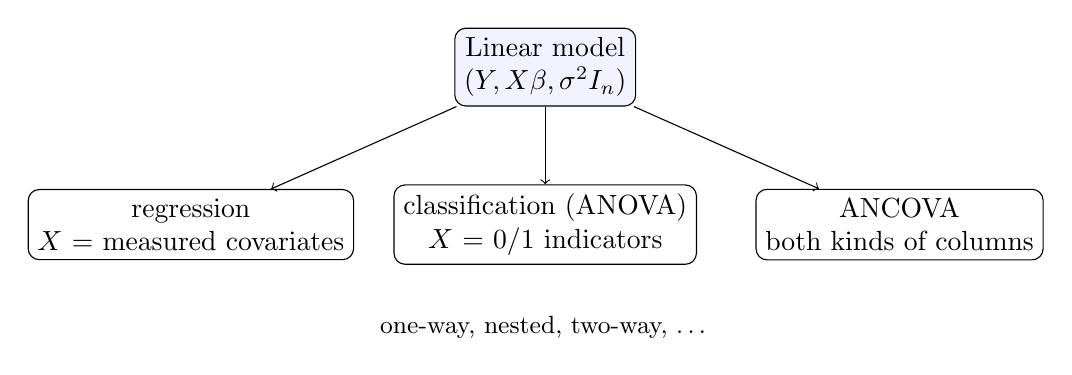
\begin{tikzpicture}[scale=1.0]
\node[draw,rounded corners,fill=blue!5,align=center] (lm) at (0,0) {Linear model\\$(Y,X\beta,\sigma^2I_n)$};
\node[draw,rounded corners,align=center] (reg) at (-4.5,-2) {regression\\$X$ = measured covariates};
\node[draw,rounded corners,align=center] (cls) at (0,-2) {classification (ANOVA)\\$X$ = 0/1 indicators};
\node[draw,rounded corners,align=center] (anc) at (4.5,-2) {ANCOVA\\both kinds of columns};
\draw[->] (lm) -- (reg); \draw[->] (lm) -- (cls); \draw[->] (lm) -- (anc);
\node[font=\small,align=center] at (0,-3.3) {one-way, nested, two-way, \dots};
\end{tikzpicture}
\caption{All models in this course are special cases of $(Y,X\beta,\sigma^2I_n)$. They differ only in the design matrix.}
\label{fig:L09-family}
\end{figure}

\subsection{Computation}
The notebook \nb{week03/L09\_theory\_linear\_models.ipynb} builds the design matrices of
\cref{ex:L09-slr,ex:L09-nested-mat} and of a two-way model with \texttt{numpy}, and also with
\texttt{patsy}/\texttt{statsmodels} formulas. It computes their ranks and checks
$\Cov(AY)=A\Cov(Y)A\T$ by simulation.

\subsection{Summary}
\begin{itemize}
  \item Linear model: $Y_i=\sum_j x_{ij}\beta_j+\eps_i$, with $\eps_i$ uncorrelated, $\EE\eps_i=0$, $\Var\eps_i=\sigma^2$. It is linear in the \emph{parameters}.
  \item Matrix form $(Y,X\beta,\sigma^2I_n)$: $Y=X\beta+\eps$, $\EE Y=X\beta$, $\Cov Y=\sigma^2I_n$.
  \item $\EE[AW+b]=A\EE W+b$ and $\Cov(AW+b)=A\Cov(W)A\T$. In particular $\Var(\ell\T Y)=\sigma^2\pnorm{\ell}^2$.
  \item Classification models (one-way, nested, two-way) are linear models with 0/1 design matrices.
\end{itemize}

\subsection{Exercises}
\begin{problem}\label{prob:L09-1}
Write the design matrix of the two-way model with interaction for $I=J=2$ and $n_{ij}=1$. What is its rank?
\end{problem}
\begin{problem}\label{prob:L09-2}
Which of the following are linear models? (a) $Y_i=\beta_1+\beta_2\sin t_i+\eps_i$; (b) $Y_i=\beta_1t_i^{\beta_2}+\eps_i$; (c) $Y_i=(\beta_1+\beta_2)t_i+\eps_i$.
\end{problem}
\begin{problem}\label{prob:L09-3}
In the linear model, find $\Cov(\bar Y,Y_1-\bar Y)$ where $\bar Y=\frac1n\sum Y_i$.
\end{problem}
\begin{problem}\label{prob:L09-4}
Let $W$ be a random vector with $\Cov(W)=\Sigma$. Show that $\Sigma$ is symmetric and positive semi-definite.
\end{problem}

\subsection{Further reading}
Christensen, \S1.1 (random vectors and matrices) and the introduction to Chapter~2. Rao, \S1b
(matrices) and \S4a.1 (the Gauss--Markoff set-up). Weisberg, \emph{ALR}, Chapter~3.

% ============================================================
% Lecture 10 -- Problem of parameter estimation
% ============================================================
\section{The Problem of Parameter Estimation}\label{sec:L10}

\lectureheader{10}{TnJ_1LZXLBk}{Week-3 handwritten notes \texttt{Feb9.pdf}, part ``The problem of estimation of the parameters'' (linear parametric functions, estimability theorem); Week-5 assignment Q2, Q5, Q6}

\begin{guiding*}
By the end of this lecture you should be able to:
\begin{itemize}
  \item define a \emph{linear parametric function} $\lambda\T\beta$ and say when it is \emph{estimable};
  \item prove that $\lambda\T\beta$ is estimable if and only if $\lambda\in\colsp{X\T}$;
  \item decide estimability in concrete models, including the one-way classification;
  \item relate estimability to the null space of $X$ and to identifiability.
\end{itemize}
\end{guiding*}

\subsection{Recap}
In the linear model $(Y,X\beta,\sigma^2I_n)$ of \cref{sec:L09}, the unknown parameters are
$\beta\in\RR^p$ and $\sigma^2>0$, i.e.\ $(\beta,\sigma^2)\in\RR^p\times\RR_+$. In
\cref{sec:L08} we saw that in the one-way model some linear combinations of $\beta$ (such as
$\mu_1-\mu_2$) have unbiased estimates, while others (such as $\mu$) cannot even be identified.
This lecture characterises the good combinations.

\subsection{Linear parametric functions}
\begin{definition}[Linear parametric function]\label{def:L10-lpf}
For $\lambda=(\lambda_1,\dots,\lambda_p)\T\in\RR^p$, the linear combination
\[
\lambda\T\beta=\lambda_1\beta_1+\lambda_2\beta_2+\dots+\lambda_p\beta_p
\]
of the parameter vector is called a \vocab{linear parametric function}.
\end{definition}
In a linear model we will be interested only in linear parametric functions. The instructor
writes $p\T\beta$ with $p\in\RR^m$; we write $\lambda\T\beta$ because $p$ denotes the number of
parameters in this book.

\begin{definition}[Estimable]\label{def:L10-estimable}
Let $(Y,X\beta,\sigma^2I_n)$ be a linear model and $\lambda\in\RR^p$. The linear parametric function
$\lambda\T\beta$ is \vocab{estimable} if there exists $\ell\in\RR^n$ such that
\[
\EE[\ell\T Y]=\lambda\T\beta\qquad\text{for every }\beta\in\RR^p .
\]
In other words, $\lambda\T\beta$ is estimable if it has a \emph{linear unbiased estimate} $\ell\T Y$.
\end{definition}
Unbiasedness must hold for every value of $\beta$. An estimate that is unbiased only for some
$\beta$'s is useless, because we do not know $\beta$.

\subsection{The estimability theorem}
\begin{theorem}[Characterisation of estimability]\label{thm:L10-estimable}
Let $(Y,X\beta,\sigma^2I_n)$ be a linear model and $\lambda\in\RR^p$. Then
\[
\lambda\T\beta \text{ is estimable}\iff \lambda\in\colsp{X\T},
\]
where $\colsp{X\T}=\{z\in\RR^p:\ z=X\T\ell\text{ for some }\ell\in\RR^n\}$ is the column space of
$X\T$, which is the row space of $X$.
\end{theorem}
\begin{proof}
We follow the chain of equivalences in the notes and justify each step.
\begin{align*}
\lambda\T\beta\text{ estimable}
&\iff \exists\,\ell\in\RR^n:\ \EE[\ell\T Y]=\lambda\T\beta\ \ \forall\beta\in\RR^p &&\text{(definition)}\\
&\iff \exists\,\ell\in\RR^n:\ \ell\T X\beta=\lambda\T\beta\ \ \forall\beta\in\RR^p &&\text{(linearity of expectation)}\\
&\iff \exists\,\ell\in\RR^n:\ X\T\ell=\lambda &&\text{(linear algebra, below)}\\
&\iff \lambda\in\colsp{X\T}. &&\text{(definition of column space)}
\end{align*}
Step 2: $\EE[\ell\T Y]=\ell\T\EE[Y]=\ell\T X\beta$ by \cref{prop:L09-rules}.
Step 3: $\ell\T X\beta=\lambda\T\beta$ for all $\beta$ means $(X\T\ell-\lambda)\T\beta=0$ for all $\beta$.
Taking $\beta=X\T\ell-\lambda$ gives $\pnorm{X\T\ell-\lambda}^2=0$, i.e.\ $X\T\ell=\lambda$. Conversely,
if $X\T\ell=\lambda$ then $\ell\T X\beta=(X\T\ell)\T\beta=\lambda\T\beta$ for all $\beta$.
\end{proof}

\begin{note}
The proof shows more than the statement. The linear unbiased estimates of $\lambda\T\beta$ are
\emph{exactly} the $\ell\T Y$ with $X\T\ell=\lambda$ (this is Week-5 assignment Q2). If some
$\ell_0$ works, then so does $\ell_0+v$ for every $v\in\nullsp{X\T}$. So there are usually many
linear unbiased estimates, and the question ``which one is best?'' (Weeks~5--6) makes sense.
\end{note}

\begin{corollary}\label{cor:L10-fullrank}
Every linear parametric function is estimable $\iff\colsp{X\T}=\RR^p\iff\rank(X)=p$.
In that case the parameters $\beta_1,\dots,\beta_p$ themselves are estimable.
\end{corollary}
\begin{proof}
All $\lambda$ lie in $\colsp{X\T}$ iff $\colsp{X\T}=\RR^p$, i.e.\ iff $\dim\colsp{X\T}=\rank(X)=p$.
Then $\beta_j=e_j\T\beta$ is estimable for each standard basis vector $e_j$.
\end{proof}

\begin{corollary}[Estimable functions form a subspace]\label{cor:L10-subspace}
If $\lambda_1\T\beta$ and $\lambda_2\T\beta$ are estimable, so is $(a\lambda_1+b\lambda_2)\T\beta$ for all
$a,b\in\RR$. Each row $x_i\T\beta=\EE Y_i$ of $X\beta$ is estimable (take $\ell=e_i$). Every estimable
function is a linear combination of these.
\end{corollary}
\begin{proof}
$\colsp{X\T}$ is a subspace spanned by the rows $x_1,\dots,x_n$ of $X$. If
$\lambda_1=X\T\ell_1$ and $\lambda_2=X\T\ell_2$ then $a\lambda_1+b\lambda_2=X\T(a\ell_1+b\ell_2)$.
\end{proof}

\begin{proposition}[Week-5 assignment Q5]\label{prop:L10-nullspace}
$\lambda\T\beta$ is estimable $\iff$ $\lambda$ is orthogonal to the null space $\nullsp{X}=\{v:Xv=0\}$.
\end{proposition}
\begin{proof}
By \cref{thm:L10-estimable} we must show $\colsp{X\T}=\nullsp{X}^\perp$.
($\subseteq$) If $\lambda=X\T\ell$ and $Xv=0$, then $\lambda\T v=\ell\T Xv=0$.
($\supseteq$) Both are subspaces of $\RR^p$. $\dim\colsp{X\T}=\rank(X)=r$, and by rank--nullity
$\dim\nullsp{X}=p-r$, so $\dim\nullsp{X}^\perp=r$. A subspace contained in another of the same
finite dimension equals it.
\end{proof}

\begin{note}[Supplementary: estimable $\Rightarrow$ identifiable]
If $\lambda\T\beta$ is estimable and $X\beta_1=X\beta_2$, then $\beta_1-\beta_2\in\nullsp{X}$, so
$\lambda\T\beta_1=\lambda\T\beta_2$ by \cref{prop:L10-nullspace}. Estimable functions are therefore
identifiable in the sense of \cref{def:L08-ident}. Conversely, a linear function that is
identifiable (constant on each set $\{\beta: X\beta=\text{const}\}$) must vanish on $\nullsp{X}$, so it
is estimable. For linear parametric functions the two notions coincide.
\end{note}

\subsection{Examples}
\begin{example}[One-way model with $k=2$, $n_1=n_2=2$]\label{ex:L10-oneway}
With $\beta=(\mu,\mu_1,\mu_2)\T$ and $Y=(Y_{11},Y_{12},Y_{21},Y_{22})\T$,
\[
X=\begin{pmatrix}1&1&0\\1&1&0\\1&0&1\\1&0&1\end{pmatrix},\qquad
\colsp{X\T}=\mathrm{span}\{(1,1,0)\T,(1,0,1)\T\}.
\]
\begin{itemize}
  \item $\mu_1-\mu_2$: $\lambda=(0,1,-1)\T=(1,1,0)\T-(1,0,1)\T\in\colsp{X\T}$, so it is \emph{estimable}. Two linear unbiased estimates are $\ell=(1,0,-1,0)\T$, i.e.\ $Y_{11}-Y_{21}$, and $\ell=(\tfrac12,\tfrac12,-\tfrac12,-\tfrac12)\T$, i.e.\ $\bar Y_{1\cdot}-\bar Y_{2\cdot}$. Both satisfy $X\T\ell=(0,1,-1)\T$. Their variances are $\sigma^2\pnorm{\ell}^2=2\sigma^2$ and $\sigma^2$ respectively.
  \item $\mu+\mu_1$: $\lambda=(1,1,0)\T$ is a row of $X$, so it is \emph{estimable} (e.g.\ by $Y_{11}$, or better by $\bar Y_{1\cdot}$).
  \item $\mu_1$: $\lambda=(0,1,0)\T$. If $a(1,1,0)+b(1,0,1)=(0,1,0)$ then $a+b=0$, $a=1$, $b=0$, a contradiction. So it is \emph{not estimable}. Equivalently, $\nullsp{X}=\mathrm{span}\{(1,-1,-1)\T\}$ and $\lambda\T(1,-1,-1)\T=-1\ne0$.
  \item $\mu$: $\lambda=(1,0,0)\T$ has $\lambda\T(1,-1,-1)\T=1\ne 0$, so it is \emph{not estimable}.
\end{itemize}
\end{example}

\begin{example}[General one-way model]\label{ex:L10-oneway-general}
In Model~1 with $\beta=(\mu,\mu_1,\dots,\mu_k)\T$, the rows of $X$ are $(1,e_i\T)$. By
\cref{prop:L08-rank}, $\nullsp{X}$ is one-dimensional, spanned by $v=(1,-1,\dots,-1)\T$.
Hence, by \cref{prop:L10-nullspace},
\[
\lambda_0\mu+\sum_{i=1}^k\lambda_i\mu_i\ \text{is estimable}\iff \lambda_0=\sum_{i=1}^k\lambda_i .
\]
Consequences: any \vocab{contrast} $\sum\lambda_i\mu_i$ with $\sum\lambda_i=0$ is estimable (e.g.\
$\mu_1-\mu_2$, $\mu_1+\mu_2-2\mu_3$), and so is $\mu+\mu_i$. The functions $\mu$ and $\mu_i$ alone are not.
This answers \cref{q:L08-questions}.
\end{example}

\begin{figure}[ht]
\centering
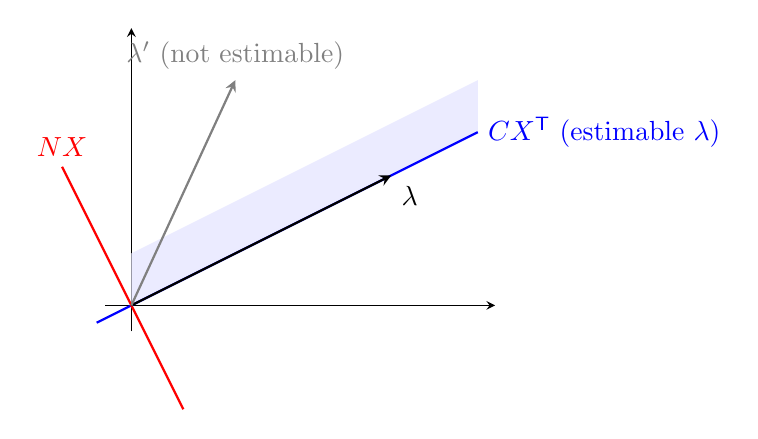
\begin{tikzpicture}[scale=1.1,>=stealth]
\draw[->] (-0.3,0) -- (4.2,0) node[right] {};
\draw[->] (0,-0.3) -- (0,3.2);
\fill[blue!8] (0,0) -- (4,2) -- (4,2.6) -- (0,0.6) -- cycle;
\draw[thick,blue] (-0.4,-0.2) -- (4,2) node[right] {$\colsp{X\T}$ (estimable $\lambda$)};
\draw[thick,red] (0.6,-1.2) -- (-0.8,1.6) node[above] {$\nullsp{X}$};
\draw[->,thick] (0,0) -- (3,1.5) node[below right] {$\lambda$};
\draw[->,thick,gray] (0,0) -- (1.2,2.6) node[above] {$\lambda'$ (not estimable)};
\end{tikzpicture}
\caption{$\lambda\T\beta$ is estimable exactly when $\lambda$ lies in the row space $\colsp{X\T}=\nullsp{X}^\perp$ (schematic, $p=2$, $\rank X=1$).}
\label{fig:L10-geom}
\end{figure}

\subsection{Computation}
To test whether $\lambda\in\colsp{X\T}$ numerically, compare $\rank(X\T)$ with $\rank([X\T\ \lambda])$,
or check whether $\lambda$ is orthogonal to a basis of $\nullsp{X}$ (\texttt{scipy.linalg.null\_space}).
A third test uses the Moore--Penrose inverse: $\lambda\in\colsp{X\T}\iff X\T(X\T)^{+}\lambda=\lambda$.
All three are implemented, and checked on \cref{ex:L10-oneway}, in
\nb{week03/L10\_estimability.ipynb}. The notebook also finds $\ell$ with $X\T\ell=\lambda$ and
verifies unbiasedness by simulation.

\subsection{Summary}
\begin{itemize}
  \item Linear parametric function: $\lambda\T\beta$. Estimable: $\exists\,\ell$ with $\EE[\ell\T Y]=\lambda\T\beta$ for all $\beta$.
  \item \textbf{Theorem:} $\lambda\T\beta$ is estimable $\iff\lambda\in\colsp{X\T}\iff\lambda\perp\nullsp{X}$. The linear unbiased estimates are $\ell\T Y$ with $X\T\ell=\lambda$.
  \item If $\rank X=p$, everything is estimable. Estimable functions form the $r$-dimensional space spanned by the rows of $X$.
  \item One-way model: $\lambda_0\mu+\sum\lambda_i\mu_i$ is estimable iff $\lambda_0=\sum\lambda_i$.
\end{itemize}

\subsection{Exercises}
\begin{problem}\label{prob:L10-1}
In the one-way model with $k=3$, decide which are estimable: $\mu$, $\mu_1-\mu_2$, $\mu+\mu_1$, $\mu_1+\mu_2-2\mu_3$, $2\mu+\mu_1+\mu_2$.
\end{problem}
\begin{problem}\label{prob:L10-2}
(Week-5 assignment Q6.) Let $k,l\ge 2$ be integers and let $X$ have rows $(1,i,ik)$ for $i=1,\dots,k$ followed by rows $(1,i,il)$ for $i=1,\dots,l$, with $\beta=(\beta_1,\beta_2,\beta_3)\T$.
(a) Show that $\beta_1$ and $\beta_2+\beta_3(l+k)/2$ are always estimable.
(b) Find a necessary and sufficient condition on $k,l$ for every linear function of $\beta$ to be estimable.
\end{problem}
\begin{problem}\label{prob:L10-3}
Show that if $\lambda\T\beta$ is estimable, then any two linear unbiased estimates $\ell_1\T Y,\ell_2\T Y$ differ by $v\T Y$ with $v\in\nullsp{X\T}$, and that $\EE[v\T Y]=0$.
\end{problem}
\begin{problem}\label{prob:L10-4}
In simple linear regression $Y_i=\beta_1+\beta_2x_i+\eps_i$, when is $\beta_2$ estimable? Relate your answer to \cref{prob:L05-4}.
\end{problem}
\begin{problem}\label{prob:L10-5}
In the nested model of \cref{ex:L09-nested-mat}, show that $\delta_{11}-\delta_{12}$ is estimable but $\mu_1-\mu_2$ is not.
\end{problem}

\subsection{Further reading}
Christensen, \S2.1 (Identifiability and Estimability), especially the result that $\lambda\T\beta$
is estimable iff $\lambda\T=\rho\T X$ for some $\rho$. Rao, \S4a.1 (estimable parametric functions).


\section*{Solutions to the Exercises of Chapter~\ref{ch:week03}}
\addcontentsline{toc}{section}{Solutions to the exercises}

\paragraph{\Cref{prob:L08-1}.}
Within group $i$, $\sum_j(Y_{ij}-\bar Y_{i\cdot})^2=\sum_j(\eps_{ij}-\bar\eps_{i\cdot})^2=\sum_j\eps_{ij}^2-n_i\bar\eps_{i\cdot}^2$.
Taking expectations, $\EE\sum_j\eps_{ij}^2=n_i\sigma^2$ and $\EE[n_i\bar\eps_{i\cdot}^2]=n_i\Var(\bar\eps_{i\cdot})=\sigma^2$.
So the expectation is $(n_i-1)\sigma^2$, and $\EE S_i^2=\sigma^2$. Summing over groups,
$\EE\,\SSW=\sum_i(n_i-1)\sigma^2=(n-k)\sigma^2$. Only $\EE\eps=0$, $\Var\eps_{ij}=\sigma^2$ and
uncorrelatedness were used.

\paragraph{\Cref{prob:L08-2}.}
Means: $2$ and $4$; grand mean $16/5=3.2$. $\SSW=(1+1)+(4+0+4)=10$.
$\SSB=2(2-3.2)^2+3(4-3.2)^2=2.88+1.92=4.8$.
$\TSS=(1-3.2)^2+(3-3.2)^2+(2-3.2)^2+(4-3.2)^2+(6-3.2)^2=4.84+0.04+1.44+0.64+7.84=14.8=10+4.8$. \checkmark

\paragraph{\Cref{prob:L08-3}.}
Let $m_i=\mu+\mu_i$ and $\bar m=\frac1n\sum n_im_i=\mu+\bar\mu_w$. Write
$\bar Y_{i\cdot}=m_i+\bar\eps_{i\cdot}$ and $\bar Y_{\cdot\cdot}=\bar m+\bar\eps_{\cdot\cdot}$. By the weighted version of
\cref{prop:L01-bestconst}, $\SSB=\sum n_i\bar Y_{i\cdot}^2-n\bar Y_{\cdot\cdot}^2$.
Now $\EE\bar Y_{i\cdot}^2=m_i^2+\sigma^2/n_i$ and $\EE\bar Y_{\cdot\cdot}^2=\bar m^2+\sigma^2/n$. Hence
$\EE\,\SSB=\sum n_im_i^2+k\sigma^2-n\bar m^2-\sigma^2=(k-1)\sigma^2+\sum n_i(m_i-\bar m)^2$, and
$m_i-\bar m=\mu_i-\bar\mu_w$.

\paragraph{\Cref{prob:L08-4}.}
From the proof of \cref{lem:L08-chisq}, $A=Q\Lambda Q\T$ with $\Lambda$ diagonal with $0/1$ entries.
Then $\tr A=\tr(\Lambda Q\T Q)=\tr\Lambda=$ the number of $1$'s $=\rank\Lambda=\rank A$.

\paragraph{\Cref{prob:L08-5}.}
$\sum_i n_im_i=n\mu+\sum n_i\mu_i=n\mu$. So $\mu=\frac1n\sum n_im_i$, which is the weighted average of
the group means, and $\mu_i=m_i-\mu$.

\paragraph{\Cref{prob:L09-1}.}
Order the observations as $(1,1)$, $(1,2)$, $(2,1)$, $(2,2)$ and the parameters as
$\mu$, $\alpha_1$, $\alpha_2$, $\beta_1$, $\beta_2$, $\gamma_{11}$, $\gamma_{12}$, $\gamma_{21}$, $\gamma_{22}$:
\[
X=\begin{pmatrix}
1&1&0&1&0&1&0&0&0\\
1&1&0&0&1&0&1&0&0\\
1&0&1&1&0&0&0&1&0\\
1&0&1&0&1&0&0&0&1
\end{pmatrix},\qquad \rank X=4
\]
(the $\gamma$ columns form $I_4$), while $p=9$.

\paragraph{\Cref{prob:L09-2}.}
(a) Linear, with $x_{i2}=\sin t_i$. (b) Not linear, because $\beta_2$ is in the exponent.
(c) The mean $(\beta_1+\beta_2)t_i$ is linear in $(\beta_1,\beta_2)$, so it is formally a linear model with
$x_{i1}=x_{i2}=t_i$. The design matrix has two equal columns, and only $\beta_1+\beta_2$ is estimable.

\paragraph{\Cref{prob:L09-3}.}
$\Cov(\bar Y,Y_1)=\frac1n\sum_l\Cov(Y_l,Y_1)=\sigma^2/n$ and $\Var(\bar Y)=\sigma^2/n$, so
$\Cov(\bar Y,Y_1-\bar Y)=0$.

\paragraph{\Cref{prob:L09-4}.}
Symmetry: $\Cov(W_i,W_l)=\Cov(W_l,W_i)$. For any $a\in\RR^n$,
$a\T\Sigma a=\Var(a\T W)\ge 0$ by \cref{prop:L09-rules}.

\paragraph{\Cref{prob:L10-1}.}
Use \cref{ex:L10-oneway-general}: $\lambda_0\mu+\sum\lambda_i\mu_i$ is estimable iff $\lambda_0=\sum\lambda_i$.
$\mu$: $1\ne0$, not estimable. $\mu_1-\mu_2$: $0=1-1$, estimable. $\mu+\mu_1$: $1=1$, estimable.
$\mu_1+\mu_2-2\mu_3$: $0=0$, estimable. $2\mu+\mu_1+\mu_2$: $2=2$, estimable. It is $(\mu+\mu_1)+(\mu+\mu_2)$.

\paragraph{\Cref{prob:L10-2}.}
Each row $(1,i,ik)=(1,0,0)+i(0,1,k)$. Since $k\ge2$, the first block contains $i=1,2$, whose rows
span $\{(1,0,0),(0,1,k)\}$. Similarly the second block spans $\{(1,0,0),(0,1,l)\}$. So
$\colsp{X\T}=\mathrm{span}\{(1,0,0),(0,1,k),(0,1,l)\}$.
(a) $(1,0,0)\T$ is in it, so $\beta_1$ is estimable. Also $(0,1,\frac{k+l}2)=\frac12(0,1,k)+\frac12(0,1,l)$ is in it,
so $\beta_2+\beta_3(k+l)/2$ is estimable, whatever $k,l$ are.
(b) $(0,1,k)$ and $(0,1,l)$ are linearly independent iff $k\ne l$. So $\rank X=3$, and every linear
function is estimable (\cref{cor:L10-fullrank}), iff $k\ne l$. If $k=l$, $\rank X=2$ and e.g.\ $\beta_3$ is
not estimable.

\paragraph{\Cref{prob:L10-3}.}
$X\T\ell_1=\lambda=X\T\ell_2$ gives $X\T(\ell_1-\ell_2)=0$, i.e.\ $v=\ell_1-\ell_2\in\nullsp{X\T}$.
Then $\EE[v\T Y]=v\T X\beta=(X\T v)\T\beta=0$.

\paragraph{\Cref{prob:L10-4}.}
$X=[\one,x]$. If the $x_i$ are not all equal, $\rank X=2=p$ and $\beta_2$ is estimable. If all
$x_i=c$, the rows are all $(1,c)$, so $\colsp{X\T}=\mathrm{span}\{(1,c)\}$. Then $(0,1)$ is not in it, and $\beta_2$
is not estimable. This matches \cref{prob:L05-4}, where the least-squares slope was not unique.

\paragraph{\Cref{prob:L10-5}.}
$\lambda=(0,0,0,1,-1,0,0)\T$ equals row 1 $-$ row 2 of $X$, so $\delta_{11}-\delta_{12}$ is estimable (by
$Y_{111}-Y_{121}$). For $\mu_1-\mu_2$, $\lambda=(0,1,-1,0,0,0,0)\T$. The vector
$v=(0,1,0,-1,-1,0,0)\T$ satisfies $Xv=0$: rows 1 and 2 give $1-1=0$, and rows 3 and 4 give $0$. But
$\lambda\T v=1\ne0$, so by \cref{prop:L10-nullspace} $\mu_1-\mu_2$ is not estimable. Only
combinations such as $(\mu_1+\frac12(\delta_{11}+\delta_{12}))-(\mu_2+\frac12(\delta_{21}+\delta_{22}))$ are estimable.

% ============================================================
% Week 4 -- Normal equations
% ============================================================
\chapter{Least Squares and the Normal Equations}\label{ch:week04}

This chapter covers Week~4 (Lectures 11--14). The instructor's handwritten notes for this week
are divided into ``Lecture 2'', ``Lecture 3'' and ``Lecture 4''. We match them to the videos by
title: the normal equations (video 12), the uniqueness theorem (video 13), and the projection
and matrix review (video 14). The first part of the notes, which recalls the models and
classifications, goes with video 11.

% ============================================================
% Lecture 11 -- Different classifications of linear models
% ============================================================
\section{Different Classifications of Linear Models}\label{sec:L11}

\lectureheader{11}{pNIF__GOLGo}{Week-4 handwritten notes \texttt{Feb14.pdf}, first part (``Recall: linear model'', examples 1--3, exercise ``express 1, 2, 3 as $(Y,X\beta,\sigma^2I)$''); Week-5 assignment Q3}

\begin{guiding*}
By the end of this lecture you should be able to:
\begin{itemize}
  \item recall the linear model $(Y,X\beta,\sigma^2I_n)$ and its ingredients;
  \item write down explicitly the design matrices of the one-way, nested and two-way classification models;
  \item compute the rank of these design matrices and say how many linear combinations of the parameters can be estimated.
\end{itemize}
\end{guiding*}

\subsection{Recall: the linear model}
The data are $n$ observations $Y_1,\dots,Y_n$, and the parameters are $\beta_1,\dots,\beta_p$ (the
notes write $m$). The model is
\[
Y_i=\sum_{j=1}^p x_{ij}\beta_j+\eps_i,\qquad \EE[\eps_i]=0,\quad \Var(\eps_i)=\sigma^2,\quad \eps_i\text{ uncorrelated},
\]
or $Y=X\beta+\eps$ with $\EE[\eps]=0$ and $\Cov(\eps)=\sigma^2I_{n}$. We write it as
$(Y,X\beta,\sigma^2I_n)$: the data, their expectation, and their variance--covariance matrix
(\cref{def:L09-matrix}).

The three examples of \cref{sec:L09} are recalled:
\begin{enumerate}
  \item one-way classification: $Y_{ij}=\mu+\mu_i+\eps_{ij}$, $1\le j\le n_i$, $1\le i\le k$;
  \item nested classification: $Y_{ijl}=\mu+\mu_i+\delta_{ij}+\eps_{ijl}$, $1\le l\le n_{ij}$, $1\le j\le m_i$, $1\le i\le k$;
  \item two-way classification: $Y_{ijl}=\mu+\alpha_i+\beta_j+\gamma_{ij}+\eps_{ijl}$, $1\le l\le n_{ij}$, $1\le j\le J$, $1\le i\le I$.
\end{enumerate}
The exercise in the notes (also Week-5 assignment Q3) is to express each of them as
$(Y,X\beta,\sigma^2I_n)$. We do this in general and then for small cases.

\subsection{A general principle}
\begin{definition}[Indicator columns]\label{def:L11-indicator}
For a classification with observations labelled by cells, the \vocab{indicator column} of a
level (or cell) $c$ is the $0/1$ vector with a $1$ exactly in the rows of observations belonging
to $c$. In all three models, $X$ is obtained by listing the observations in a fixed order (say
lexicographic in $(i,j,l)$) and writing one column for each parameter: $\one_n$ for $\mu$, and the
indicator column of the corresponding level or cell for every other parameter.
\end{definition}
Indeed, the coefficient of a parameter in the equation for $Y_{ijl}$ is $1$ if the parameter
appears in that equation and $0$ otherwise.

\subsection{Model 1: one-way classification}
\begin{example}[$k=3$, $n_1=n_2=n_3=2$]\label{ex:L11-oneway}
$Y=(Y_{11},Y_{12},Y_{21},Y_{22},Y_{31},Y_{32})\T$ and $\beta=(\mu,\mu_1,\mu_2,\mu_3)\T$:
\[
X=\begin{pmatrix}
1&1&0&0\\1&1&0&0\\1&0&1&0\\1&0&1&0\\1&0&0&1\\1&0&0&1
\end{pmatrix},\qquad n=6,\ p=4,\ \rank X=3 .
\]
\end{example}
By \cref{prop:L08-rank}, $\rank X=k$ in general.

\subsection{Model 2: nested classification}
\begin{example}[$k=2$, $m_1=m_2=2$, $n_{ij}=2$]\label{ex:L11-nested}
$\beta=(\mu,\mu_1,\mu_2,\delta_{11},\delta_{12},\delta_{21},\delta_{22})\T$ and
$Y=(Y_{111},Y_{112},Y_{121},Y_{122},Y_{211},Y_{212},Y_{221},Y_{222})\T$:
\[
X=\begin{pmatrix}
1&1&0&1&0&0&0\\
1&1&0&1&0&0&0\\
1&1&0&0&1&0&0\\
1&1&0&0&1&0&0\\
1&0&1&0&0&1&0\\
1&0&1&0&0&1&0\\
1&0&1&0&0&0&1\\
1&0&1&0&0&0&1
\end{pmatrix},\qquad n=8,\ p=7,\ \rank X=4 .
\]
\end{example}

\begin{proposition}\label{prop:L11-nestedrank}
In the nested model with every $n_{ij}\ge1$, $\rank X=\sum_{i=1}^k m_i$, the number of subgroups.
\end{proposition}
\begin{proof}
Let $d_{ij}$ be the indicator column of subgroup $(i,j)$. These columns are non-zero and have
disjoint supports, so, as in the proof of \cref{prop:L08-rank}, they are linearly independent.
The remaining columns are sums of them: the column of $\mu_i$ is $\sum_{j=1}^{m_i}d_{ij}$ and the
column of $\mu$ is $\sum_{i,j}d_{ij}$. Hence $\colsp{X}=\mathrm{span}\{d_{ij}\}$, which has dimension $\sum_i m_i$.
\end{proof}

\subsection{Model 3: two-way classification}
\begin{example}[$I=J=2$, $n_{ij}=2$]\label{ex:L11-twoway}
$\beta=(\mu,\alpha_1,\alpha_2,\beta_1,\beta_2,\gamma_{11},\gamma_{12},\gamma_{21},\gamma_{22})\T$ and $Y$
ordered as $Y_{111},Y_{112},Y_{121},Y_{122},Y_{211},Y_{212},Y_{221},Y_{222}$:
\[
X=\begin{pmatrix}
1&1&0&1&0&1&0&0&0\\
1&1&0&1&0&1&0&0&0\\
1&1&0&0&1&0&1&0&0\\
1&1&0&0&1&0&1&0&0\\
1&0&1&1&0&0&0&1&0\\
1&0&1&1&0&0&0&1&0\\
1&0&1&0&1&0&0&0&1\\
1&0&1&0&1&0&0&0&1
\end{pmatrix},\qquad n=8,\ p=9,\ \rank X=4 .
\]
\end{example}

\begin{proposition}\label{prop:L11-tworank}
In the two-way model with interaction and every $n_{ij}\ge1$, $\rank X=IJ$, the number of cells.
In the \emph{additive} two-way model $Y_{ijl}=\mu+\alpha_i+\beta_j+\eps_{ijl}$ (no $\gamma_{ij}$), with every
$n_{ij}\ge 1$, $\rank X=I+J-1$.
\end{proposition}
\begin{proof}
With interaction: the $IJ$ cell indicators $g_{ij}$ (the columns of the $\gamma_{ij}$) are non-zero with disjoint
supports, so they are independent. The other columns are sums of them: $\alpha_i\mapsto\sum_j g_{ij}$,
$\beta_j\mapsto\sum_i g_{ij}$, $\mu\mapsto\sum_{i,j}g_{ij}$. So $\colsp{X}=\mathrm{span}\{g_{ij}\}$ has dimension $IJ$.

Additive model: the columns are $\one$, $a_i=\sum_j g_{ij}$ and $b_j=\sum_i g_{ij}$. Since
$\sum_i a_i=\sum_jb_j=\one$, the column space is spanned by $a_1,\dots,a_I,b_1,\dots,b_J$, and there is at least the one
relation $\sum a_i-\sum b_j=0$. So the rank is at most $I+J-1$. To see that it is exactly $I+J-1$, suppose
$\sum_i s_ia_i+\sum_j t_jb_j=0$. Every cell is non-empty, so reading the row of an observation in
cell $(i,j)$ gives $s_i+t_j=0$ for all $i,j$. Hence $s_i=-t_1$ for all $i$ and $t_j=-s_1$ for all $j$, so
all $s_i$ equal some $s$ and all $t_j=-s$. The relations form a $1$-dimensional space, so the
$I+J$ columns $a_i,b_j$ span a space of dimension $I+J-1$.
\end{proof}

\begin{note}[How many parameters can we estimate?]
The rank tells us how many linearly independent linear parametric functions are estimable
(\cref{cor:L10-subspace}): $k$ of the $k+1$ in Model~1, $\sum m_i$ of the $1+k+\sum m_i$ in Model~2,
and $IJ$ of the $1+I+J+IJ$ in Model~3. The estimable functions are exactly the combinations of
cell means. In the next lectures we find \emph{how} to estimate them: by least squares.
\end{note}

\begin{note}[Supplementary: Kronecker-product form]
With equal replication the design matrices have a compact form. In Model~1 with $n_i\equiv m$:
$X=[\one_k\otimes\one_m,\ I_k\otimes\one_m]$. In Model~3 with $n_{ij}\equiv m$:
$X=[\one_I\otimes\one_J\otimes\one_m,\ I_I\otimes\one_J\otimes\one_m,\ \one_I\otimes I_J\otimes\one_m,\ I_I\otimes I_J\otimes\one_m]$.
The notebook builds the matrices of this lecture both ways.
\end{note}

\subsection{Computation}
\nb{week04/L11\_classification\_designs.ipynb} writes a general function that builds the design
matrix from factor labels, checks the ranks of \cref{prop:L11-nestedrank,prop:L11-tworank}, and
compares with the full-rank codings that \texttt{statsmodels} formulas produce.

\subsection{Summary}
\begin{itemize}
  \item Each parameter contributes one column: $\one$ for $\mu$, an indicator column for each level or cell effect.
  \item Ranks: one-way $k$; nested $\sum m_i$; two-way with interaction $IJ$; additive two-way $I+J-1$ (all cells non-empty).
  \item The rank is the number of linearly independent estimable functions.
\end{itemize}

\subsection{Exercises}
\begin{problem}\label{prob:L11-1}
Write the design matrix of the additive two-way model with $I=2$, $J=3$, $n_{ij}=1$, and verify that its rank is $4$.
\end{problem}
\begin{problem}\label{prob:L11-2}
In the two-way model with interaction, $I=J=2$, suppose cell $(2,2)$ is empty. What is $\rank X$ now?
\end{problem}
\begin{problem}\label{prob:L11-3}
In the nested model, show that $\mu+\mu_i+\delta_{ij}$ is estimable for each subgroup, and give a linear unbiased estimate.
\end{problem}
\begin{problem}\label{prob:L11-4}
Show that in the additive two-way model $\alpha_1-\alpha_2$ is estimable when all cells are non-empty.
\end{problem}

\subsection{Further reading}
Christensen, Chapter~4 (one-way ANOVA), Chapter~7 (multifactor ANOVA) and Chapter~8 (nested
models); Rao, \S4d (analysis of variance, two-way and nested classifications).

% ============================================================
% Lecture 12 -- Normal equations and existence of least square estimates
% ============================================================
\section{Normal Equations and Existence of Least Squares Estimates}\label{sec:L12}

\lectureheader{12}{Ek-3Ph1AFes}{Week-4 handwritten notes \texttt{Feb14.pdf}, part ``Least square estimation'' and ``Lecture 2'' (normal equations, proof of the theorem)}

\begin{guiding*}
By the end of this lecture you should be able to:
\begin{itemize}
  \item define a least squares estimate of $\beta$ and of a linear parametric function;
  \item derive the \emph{normal equations} $X\T X\beta=X\T Y$ and prove that their solutions are exactly the least squares estimates;
  \item prove that the normal equations always have a solution, although it need not be unique;
  \item picture least squares as dropping a perpendicular from $Y$ onto the column space of $X$.
\end{itemize}
\end{guiding*}

\subsection{Recap and motivation}
In Week~2 we found the best line by minimising $\sum_i(y_i-a_1-a_2x_i)^2$
(\cref{thm:L05-slr}). We now do the same for a general linear model $(Y,X\beta,\sigma^2I_n)$, where
$X$ may have any number of columns and need not have full rank. Recall that for $z\in\RR^n$,
$\pnorm{z}^2=\sum_i z_i^2$ is the squared distance of $z$ from the origin. So
$\pnorm{Y-X\beta}^2=\sum_i\bigl(Y_i-\sum_j x_{ij}\beta_j\bigr)^2$ is the squared distance between the data and
the point $X\beta$.

\subsection{Least squares estimates}
\begin{definition}[Least squares estimate]\label{def:L12-lse}
Let $(Y,X\beta,\sigma^2I_n)$ be a linear model. A (random) vector $\hat\beta\in\RR^p$ is a
\vocab{least squares estimate} of $\beta$ if
\[
\pnorm{Y-X\hat\beta}^2=\min_{\beta\in\RR^p}\pnorm{Y-X\beta}^2 .
\]
For a linear parametric function $\lambda\T\beta$, the least squares estimate is $\lambda\T\hat\beta$.
We write $R_0^2=\min_\beta\pnorm{Y-X\beta}^2$ for the minimum. It is called the \vocab{residual sum
of squares} ($\RSS$ or $\SSE$).
\end{definition}

\begin{remark}\label{rem:L12-closest}
The definition requires that $X\hat\beta$ be the point \emph{closest} to $Y$ among all possible
choices of $X\beta$, $\beta\in\RR^p$, i.e.\ among all points of the column space $\colsp{X}$.
\end{remark}

\subsection{The normal equations}
\begin{theorem}[Normal equations]\label{thm:L12-normal}
Consider a linear model $(Y,X\beta,\sigma^2I_n)$.
\begin{enumerate}
  \item The \vocab{normal equations}
  \begin{equation}\label{eq:L12-normal}
  X\T X\,\beta=X\T Y
  \end{equation}
  always have at least one solution.
  \item $\hat\beta$ is a least squares estimate of $\beta$ if and only if it solves \eqref{eq:L12-normal}.
  \item If $\tilde\beta$ is any solution of \eqref{eq:L12-normal}, then for every $\beta\in\RR^p$
  \begin{equation}\label{eq:L12-pyth}
  \pnorm{Y-X\beta}^2=\pnorm{Y-X\tilde\beta}^2+\pnorm{X(\tilde\beta-\beta)}^2,
  \end{equation}
  and $R_0^2=\pnorm{Y-X\tilde\beta}^2$.
\end{enumerate}
\end{theorem}
The remark in the notes: a solution \emph{need not be unique}, but it always \emph{exists}, and that is
all we show here. Uniqueness is the subject of \cref{sec:L13}. The proof uses the following fact
from linear algebra, which is proved in \cref{sec:L14} (\cref{thm:L14-colspace}).

\begin{lemma}\label{lem:L12-colspace}
For every matrix $X$, $\colsp{X\T X}=\colsp{X\T}$.
\end{lemma}

\begin{proof}[Proof of \cref{thm:L12-normal}]
\emph{Existence.} First of all, $X\T Y\in\colsp{X\T}=\colsp{X\T X}$ by \cref{lem:L12-colspace}. By the
definition of a column space, there exists $\tilde\beta\in\RR^p$ with $(X\T X)\tilde\beta=X\T Y$.

\emph{The identity \eqref{eq:L12-pyth}.} Let $\tilde\beta$ solve the normal equations and let $\beta\in\RR^p$ be
arbitrary. Add and subtract $X\tilde\beta$:
\[
\pnorm{Y-X\beta}^2=\pnorm{(Y-X\tilde\beta)+X(\tilde\beta-\beta)}^2 .
\]
For $u,w\in\RR^n$ we have $\pnorm{u+w}^2=\sum_i(u_i+w_i)^2=\pnorm u^2+\pnorm w^2+2\langle u,w\rangle$, where
$\langle u,w\rangle=u\T w=\sum_iu_iw_i$. Hence
\[
\pnorm{Y-X\beta}^2=\pnorm{Y-X\tilde\beta}^2+\pnorm{X(\tilde\beta-\beta)}^2+2\langle Y-X\tilde\beta,\,X(\tilde\beta-\beta)\rangle .
\]
We now understand the cross term. It is a scalar, so it equals its own transpose:
\[
\langle Y-X\tilde\beta,\,X(\tilde\beta-\beta)\rangle=(Y-X\tilde\beta)\T X(\tilde\beta-\beta)=(\tilde\beta-\beta)\T X\T(Y-X\tilde\beta)
=(\tilde\beta-\beta)\T\bigl(X\T Y-X\T X\tilde\beta\bigr)=0,
\]
by the choice of $\tilde\beta$. This proves \eqref{eq:L12-pyth}.

\emph{Solutions are least squares estimates.} From \eqref{eq:L12-pyth},
$\pnorm{Y-X\beta}^2\ge\pnorm{Y-X\tilde\beta}^2$ for every $\beta$, so $\tilde\beta$ attains the minimum and
$R_0^2=\pnorm{Y-X\tilde\beta}^2$.

\emph{Least squares estimates are solutions.} Let $\hat\beta$ be a least squares estimate and fix a solution
$\tilde\beta$. Then $\pnorm{Y-X\hat\beta}^2=R_0^2=\pnorm{Y-X\tilde\beta}^2$, and \eqref{eq:L12-pyth} with
$\beta=\hat\beta$ gives $\pnorm{X(\tilde\beta-\hat\beta)}^2=0$, i.e.\ $X\hat\beta=X\tilde\beta$. Therefore
$X\T X\hat\beta=X\T X\tilde\beta=X\T Y$.
\end{proof}

\begin{corollary}\label{cor:L12-fitted}
All least squares estimates give the same fitted vector $\hat Y=X\hat\beta$ and the same residual
vector $\hat e=Y-X\hat\beta$. The residual vector is orthogonal to every column of $X$: $X\T\hat e=0$.
If $\rank X=p$, then $X\T X$ is invertible and $\hat\beta=(X\T X)^{-1}X\T Y$ is the unique least squares estimate.
\end{corollary}
\begin{proof}
The first statement was shown at the end of the proof above. $X\T\hat e=X\T Y-X\T X\hat\beta=0$ is the normal
equations. If $\rank X=p$ then $\rank X\T X=\rank X=p$ by \cref{lem:L12-colspace}. The $p\times p$
matrix $X\T X$ is then invertible, and \eqref{eq:L12-normal} has exactly one solution.
\end{proof}

\begin{figure}[ht]
\centering
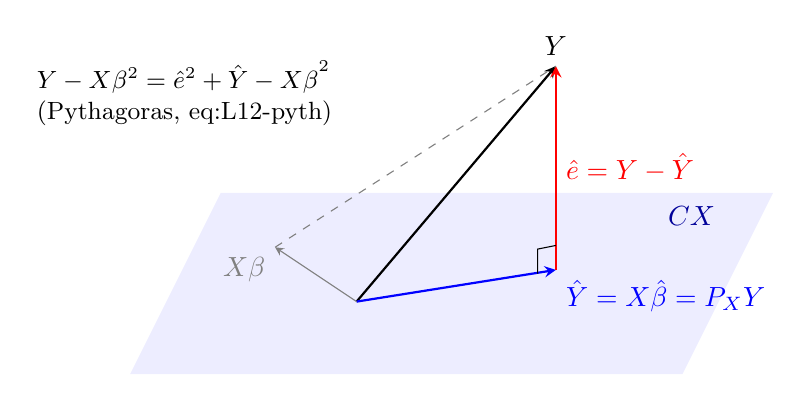
\begin{tikzpicture}[scale=1.15,>=stealth]
\fill[blue!7] (-2.5,-0.8) -- (3.6,-0.8) -- (4.6,1.2) -- (-1.5,1.2) -- cycle;
\node[blue!60!black] at (3.7,0.95) {$\colsp{X}$};
\coordinate (O) at (0,0);
\coordinate (P) at (2.2,0.35);
\coordinate (Y) at (2.2,2.6);
\coordinate (Q) at (-0.9,0.6);
\draw[->,thick] (O) -- (Y) node[above] {$Y$};
\draw[->,thick,blue] (O) -- (P) node[below right] {$\hat Y=X\hat\beta=\PX Y$};
\draw[->,thick,red] (P) -- (Y) node[midway,right] {$\hat e=Y-\hat Y$};
\draw[->,gray] (O) -- (Q) node[below left] {$X\beta$};
\draw[dashed,gray] (Q) -- (Y);
\draw (2.2,0.62) -- (2.0,0.58) -- (2.0,0.31);
\node[font=\small,align=left] at (-1.9,2.3) {$\pnorm{Y-X\beta}^2=\pnorm{\hat e}^2+\pnorm{\hat Y-X\beta}^2$\\(Pythagoras, \eqref{eq:L12-pyth})};
\end{tikzpicture}
\caption{Least squares geometry. $X\hat\beta$ is the foot of the perpendicular from $Y$ to the plane $\colsp{X}$. The residual $\hat e$ is orthogonal to $\colsp{X}$ (the normal equations), and every other $X\beta$ is farther from $Y$.}
\label{fig:L12-geometry}
\end{figure}

The name ``normal'' refers to this picture: the residual is \emph{normal} (perpendicular) to the
column space.

\begin{example}[Simple linear regression in matrix form]\label{ex:L12-slr}
Take $x=(1,2,3,4)$, $Y=(2,3,5,6)\T$ and $X=[\one,x]$ as in \cref{ex:L09-slr}. Then
\[
X\T X=\begin{pmatrix}4&10\\10&30\end{pmatrix},\qquad X\T Y=\begin{pmatrix}16\\47\end{pmatrix},\qquad
\det(X\T X)=120-100=20 .
\]
So
\[
\hat\beta=(X\T X)^{-1}X\T Y=\frac1{20}\begin{pmatrix}30&-10\\-10&4\end{pmatrix}\begin{pmatrix}16\\47\end{pmatrix}
=\frac1{20}\begin{pmatrix}480-470\\-160+188\end{pmatrix}=\begin{pmatrix}0.5\\1.4\end{pmatrix},
\]
exactly as in \cref{ex:L05-hand}, with $R_0^2=0.2$. Written out, the two normal equations
are $\sum_i\hat e_i=0$ and $\sum_ix_i\hat e_i=0$ (\cref{cor:L05-props}).
\end{example}

\begin{example}[A rank-deficient model: many solutions]\label{ex:L12-oneway}
One-way model, $k=2$, $n_1=n_2=2$, $\beta=(\mu,\mu_1,\mu_2)\T$ and data $Y=(3,5,8,10)\T$. With $X$ from
\cref{ex:L10-oneway}:
\[
X\T X=\begin{pmatrix}4&2&2\\2&2&0\\2&0&2\end{pmatrix},\qquad X\T Y=\begin{pmatrix}26\\8\\18\end{pmatrix}.
\]
The normal equations are $4\mu+2\mu_1+2\mu_2=26$, $2\mu+2\mu_1=8$, $2\mu+2\mu_2=18$. The first is the sum of the other
two, so they reduce to $\mu+\mu_1=4$ and $\mu+\mu_2=9$. The solution set is the line
\[
\hat\beta(t)=(t,\ 4-t,\ 9-t)\T,\qquad t\in\RR .
\]
Every $\hat\beta(t)$ gives the same fitted vector $X\hat\beta(t)=(4,4,9,9)\T$ (the group means), the same
residuals $(-1,1,-1,1)\T$, and $R_0^2=4$. The solution with the smallest norm minimises
$t^2+(4-t)^2+(9-t)^2$. Setting the derivative to zero gives $3t=13$, so $t=13/3$ and
$\hat\beta=(13/3,-1/3,14/3)\T$. This is the solution returned by the Moore--Penrose inverse (below).
\end{example}

\begin{note}[Supplementary: solutions via a generalized inverse]
A \vocab{generalized inverse} of a matrix $A$ is any matrix $\ginv A$ with $A\ginv AA=A$. Every matrix has one; the
Moore--Penrose inverse $A^{+}$ (\texttt{numpy.linalg.pinv}) is a particular choice. Then
\[
\hat\beta=\ginv{(X\T X)}X\T Y
\]
solves the normal equations. By \cref{lem:L12-colspace}, $X\T Y=X\T Xb$ for some $b$, so
$X\T X\,\ginv{(X\T X)}X\T Y=X\T X\,\ginv{(X\T X)}X\T Xb=X\T Xb=X\T Y$. With $A^{+}$ one gets the minimum-norm
solution of \cref{ex:L12-oneway}.
\end{note}

\subsection{Computation}
\nb{week04/L12\_normal\_equations.ipynb} solves the normal equations for both examples
(\texttt{numpy.linalg.solve} for full rank; \texttt{pinv} and \texttt{lstsq} for rank-deficient $X$). It
checks the Pythagorean identity \eqref{eq:L12-pyth} numerically, shows that different solutions give
the same fitted values, and compares with \texttt{statsmodels} OLS.

\subsection{Summary}
\begin{itemize}
  \item $\hat\beta$ is a least squares estimate iff it minimises $\pnorm{Y-X\beta}^2$ iff $X\T X\hat\beta=X\T Y$.
  \item Solutions always exist, because $X\T Y\in\colsp{X\T}=\colsp{X\T X}$. They are unique iff $\rank X=p$, in which case $\hat\beta=(X\T X)^{-1}X\T Y$.
  \item Pythagoras: $\pnorm{Y-X\beta}^2=\pnorm{Y-X\hat\beta}^2+\pnorm{X(\hat\beta-\beta)}^2$.
  \item The fitted values $X\hat\beta$ and the residuals are the same for every solution, and $X\T\hat e=0$.
\end{itemize}

\subsection{Exercises}
\begin{problem}\label{prob:L12-1}
Write the normal equations for $Y_i=\beta_1+\beta_2x_i+\eps_i$ in terms of $\sum x_i$, $\sum x_i^2$, $\sum Y_i$, $\sum x_iY_i$, and solve them to recover \cref{thm:L05-slr}.
\end{problem}
\begin{problem}\label{prob:L12-2}
For the one-way model with general $k$ and $n_i$, show that the normal equations reduce to $\mu+\mu_i=\bar Y_{i\cdot}$, $i=1,\dots,k$, and that $R_0^2=\SSW$.
\end{problem}
\begin{problem}\label{prob:L12-3}
Show that $\sum_i\hat e_i=0$ whenever $\one_n\in\colsp{X}$.
\end{problem}
\begin{problem}\label{prob:L12-4}
Verify that $G=\mathrm{diag}(0,\tfrac12,\tfrac12)$ is a generalized inverse of $X\T X$ in \cref{ex:L12-oneway}, and find the corresponding solution $GX\T Y$.
\end{problem}

\subsection{Further reading}
Christensen, \S2.2 (least squares estimation) and Appendix~B (generalized inverses); Rao, \S4a.2
(normal equations) and \S1b.5 (generalized inverse of a matrix).

% ============================================================
% Lecture 13 -- Theorem on least square estimates
% ============================================================
\section{A Theorem on Least Squares Estimates}\label{sec:L13}

\lectureheader{13}{XLT3vSQphCg}{Week-4 handwritten notes \texttt{Feb14.pdf}, part ``Lecture 3'' (estimable $\iff$ least squares estimate unique)}

\begin{guiding*}
By the end of this lecture you should be able to:
\begin{itemize}
  \item state and prove: $\lambda\T\beta$ is estimable if and only if its least squares estimate $\lambda\T\hat\beta$ is the same for every solution $\hat\beta$ of the normal equations;
  \item compute the least squares estimate of an estimable function in a rank-deficient model;
  \item show that the least squares estimate of an estimable function is a \emph{linear unbiased} estimate.
\end{itemize}
\end{guiding*}

\subsection{Recall}
For the linear model $(Y,X\beta,\sigma^2I_n)$ and $\lambda\in\RR^p$, the linear parametric function
$\lambda\T\beta$ is estimable if there is $\ell\in\RR^n$ with $\EE[\ell\T Y]=\lambda\T\beta$ for all $\beta$, i.e.\ if
$\ell\T Y$ is an unbiased estimate of $\lambda\T\beta$. By \cref{thm:L10-estimable} this happens iff
$\lambda\in\colsp{X\T}$. In \cref{sec:L12} we saw that the normal equations may have many solutions
(\cref{ex:L12-oneway}). So the ``least squares estimate'' $\lambda\T\hat\beta$ might depend on which solution we
pick. The theorem of this lecture says exactly when it does not.

\subsection{The theorem}
\begin{theorem}\label{thm:L13-unique}
Let $(Y,X\beta,\sigma^2I_n)$ be a linear model and $\lambda\in\RR^p$. Then $\lambda\T\beta$ is estimable if and
only if its least squares estimate is unique, i.e.\ $\lambda\T\hat\beta_1=\lambda\T\hat\beta_2$ for any two
solutions $\hat\beta_1,\hat\beta_2$ of the normal equations $X\T X\beta=X\T Y$.
\end{theorem}
\begin{proof}
($\Rightarrow$) Suppose $\lambda\T\beta$ is estimable. Then $\lambda\in\colsp{X\T}=\colsp{X\T X}$ (recall the earlier
theorem, \cref{thm:L10-estimable}, and \cref{lem:L12-colspace}). So there exists $b\in\RR^p$ with
$\lambda=X\T Xb$. Let $\hat\beta$ be any solution of the normal equations. Then
\[
\lambda\T\hat\beta=(X\T Xb)\T\hat\beta=b\T X\T X\hat\beta=b\T X\T Y ,
\]
which does not depend on the choice of $\hat\beta$. Hence the least squares estimate of $\lambda\T\beta$
is unique.

($\Leftarrow$) Suppose $\lambda\T\hat\beta$ is the same for all solutions $\hat\beta$. Take one solution $\hat\beta_1$ and any
$v\in\nullsp{X\T X}$, i.e.\ $X\T Xv=0$. Then $\hat\beta_2=\hat\beta_1+v$ is also a solution:
$X\T X\hat\beta_2=X\T X\hat\beta_1+0=X\T Y$. By assumption $\lambda\T\hat\beta_2=\lambda\T\hat\beta_1$, i.e.\ $\lambda\T v=0$. So $\lambda$ is
orthogonal to $\nullsp{X\T X}$. For the symmetric matrix $A=X\T X$,
\[
\nullsp{A}^\perp=\colsp{A\T}=\colsp{A}
\]
(the proof of \cref{prop:L10-nullspace} applied to $A$). Hence
$\lambda\in\colsp{X\T X}=\colsp{X\T}$ (\cref{lem:L12-colspace}), and $\lambda\T\beta$ is estimable by \cref{thm:L10-estimable}.
\end{proof}

\begin{note}
The set of all solutions of the normal equations is $\hat\beta_1+\nullsp{X\T X}$, and
$\nullsp{X\T X}=\nullsp{X}$ (\cref{thm:L14-colspace}). The theorem therefore says: $\lambda\T\hat\beta$ is constant on
this affine set iff $\lambda\perp\nullsp{X}$. This is the condition of \cref{prop:L10-nullspace}, now seen
from the side of the estimates rather than the side of the expectations.
\end{note}

\begin{proposition}[Least squares estimates of estimable functions are unbiased]\label{prop:L13-unbiased}
If $\lambda\T\beta$ is estimable, with $\lambda=X\T\ell$, then its least squares estimate satisfies
\[
\lambda\T\hat\beta=\ell\T X\hat\beta=\ell\T\hat Y,
\]
which is a linear function of $Y$, and $\EE[\lambda\T\hat\beta]=\lambda\T\beta$.
\end{proposition}
\begin{proof}
$\lambda\T\hat\beta=\ell\T X\hat\beta$ holds for every solution. By \cref{cor:L12-fitted}, $X\hat\beta=\hat Y$ is the same for
all solutions. In the proof of \cref{thm:L13-unique} we wrote $\lambda\T\hat\beta=b\T X\T Y$, which is linear in $Y$.
Then $\EE[b\T X\T Y]=b\T X\T X\beta=(X\T Xb)\T\beta=\lambda\T\beta$.
\end{proof}
Thus, for an estimable $\lambda\T\beta$, $\lambda\T\hat\beta$ is one of the linear unbiased estimates of \cref{sec:L10}.
Week~6 (the Gauss--Markov theorem) shows that it is the \emph{best} one.

\subsection{Examples}
\begin{example}[Continuing \cref{ex:L12-oneway}]\label{ex:L13-oneway}
The solutions are $\hat\beta(t)=(t,4-t,9-t)\T$, $t\in\RR$, and $\nullsp{X}=\mathrm{span}\{(1,-1,-1)\T\}$.
\begin{itemize}
  \item $\mu_1-\mu_2$, $\lambda=(0,1,-1)\T$: $\lambda\T\hat\beta(t)=(4-t)-(9-t)=-5$ for every $t$. It is unique, as the theorem predicts for an estimable function. The estimate is $\bar Y_{1\cdot}-\bar Y_{2\cdot}=4-9$.
  \item $\mu+\mu_2$, $\lambda=(1,0,1)\T$: $t+9-t=9=\bar Y_{2\cdot}$ for every $t$.
  \item $\mu_1$, $\lambda=(0,1,0)\T$: $\lambda\T\hat\beta(t)=4-t$ depends on $t$. It is not unique, so $\mu_1$ is not estimable.
  \item $\mu$: $\hat\mu=t$ can be any real number. With the constraint $\mu_1+\mu_2=0$ of \cref{prop:L08-constraint}, we would pick $t$ with $(4-t)+(9-t)=0$, i.e.\ $t=6.5$, so $\hat\beta=(6.5,-2.5,2.5)\T$.
\end{itemize}
\end{example}

\begin{example}[A regression design with a redundant column]\label{ex:L13-collinear}
Let $Y_i=\beta_1+\beta_2x_i+\beta_3z_i+\eps_i$ with $z_i=2x_i$ for all $i$ (for example, the same length recorded in two
units). Then $\nullsp{X}=\mathrm{span}\{(0,2,-1)\T\}$. The function $\beta_2+2\beta_3$ (the total effect of $x$) is
estimable, since $(0,1,2)\cdot(0,2,-1)=0$. The separate slopes $\beta_2$ and $\beta_3$ are not. Software fitting
this model must either drop a column or report a warning: \texttt{statsmodels} uses the
Moore--Penrose solution and flags a singular design. The notebook shows this with the data of
\cref{ex:L12-slr}.
\end{example}

\subsection{Computation}
\nb{week04/L13\_uniqueness\_of\_lse.ipynb} generates many solutions $\hat\beta+v$, $v\in\nullsp{X}$, of the
normal equations and plots $\lambda\T\hat\beta$ for estimable and non-estimable $\lambda$ (constant versus varying).
It also verifies \cref{prop:L13-unbiased} by simulation.

\subsection{Summary}
\begin{itemize}
  \item \textbf{Theorem:} $\lambda\T\beta$ is estimable $\iff$ $\lambda\T\hat\beta$ is the same for all solutions of $X\T X\beta=X\T Y$.
  \item If $\lambda=X\T Xb$, then $\lambda\T\hat\beta=b\T X\T Y$. If $\lambda=X\T\ell$, then $\lambda\T\hat\beta=\ell\T\hat Y$. It is linear in $Y$ and unbiased.
  \item Non-estimable functions (like $\mu$ or $\mu_i$ in the one-way model) have least squares ``estimates'' that depend on an arbitrary choice.
\end{itemize}

\subsection{Exercises}
\begin{problem}\label{prob:L13-1}
In the one-way model with general $k$, show that the least squares estimate of an estimable contrast $\sum_i c_i\mu_i$ ($\sum c_i=0$) is $\sum_i c_i\bar Y_{i\cdot}$.
\end{problem}
\begin{problem}\label{prob:L13-2}
Show that $\Var(\lambda\T\hat\beta)=\sigma^2\,\lambda\T\ginv{(X\T X)}\lambda$ for estimable $\lambda\T\beta$ and any generalized inverse, and that the value does not depend on the choice of $\ginv{(X\T X)}$.
\end{problem}
\begin{problem}\label{prob:L13-3}
In \cref{ex:L13-collinear}, find all solutions of the normal equations for $x=(1,2,3,4)$, $z=2x$, $Y=(2,3,5,6)\T$, and the least squares estimate of $\beta_2+2\beta_3$.
\end{problem}
\begin{problem}\label{prob:L13-4}
Give an example where $\lambda\T\hat\beta$ is the same for two particular solutions but $\lambda\T\beta$ is not estimable. Why does this not contradict the theorem?
\end{problem}

\subsection{Further reading}
Christensen, \S2.2 (Theorem 2.2.3 and the discussion of estimable functions and least squares).
Rao, \S4a.2 (least squares estimators of estimable functions are unique).

% ============================================================
% Lecture 14 -- Fundamentals of matrices
% ============================================================
\section{Fundamentals of Matrices and the Projection $P_X$}\label{sec:L14}

\lectureheader{14}{K_j3NHsQ4t8}{Week-4 handwritten notes \texttt{Feb14.pdf}, part ``Lecture 4'' (proposition on $X\beta$ and $P_X$; linear algebra review of the four subspaces, $\nullsp{A}=\nullsp{A\T A}$, rank--nullity)}

\begin{guiding*}
By the end of this lecture you should be able to:
\begin{itemize}
  \item show that $X\beta$ is estimable and that its least squares estimate is $X\hat\beta=\PX Y$, the orthogonal projection of $Y$ onto $\colsp{X}$;
  \item work with the four fundamental subspaces of a matrix, and compute them for small examples;
  \item prove $\nullsp{A}=\nullsp{A\T A}$ and $\colsp{A\T A}=\colsp{A\T}$ using the rank--nullity theorem;
  \item construct $\PX$ and list its properties.
\end{itemize}
\end{guiding*}

\subsection{Recap}
Least squares estimates are the solutions of $X\T X\beta=X\T Y$ (\cref{thm:L12-normal}). The estimate of $\lambda\T\beta$
is unique exactly when $\lambda\T\beta$ is estimable (\cref{thm:L13-unique}). Both proofs used
$\colsp{X\T X}=\colsp{X\T}$ (\cref{lem:L12-colspace}). This lecture proves it and identifies the fitted vector
geometrically.

\subsection{$X\beta$ and the orthogonal projection}
\begin{definition}[Orthogonal projection]\label{def:L14-proj}
Let $V\subseteq\RR^n$ be a subspace. A vector $w\in V$ is the \vocab{orthogonal projection} of $y\in\RR^n$ onto $V$ if
$y-w\perp V$, i.e.\ $\langle y-w,v\rangle=0$ for all $v\in V$. The matrix $P_V$ with $P_Vy=$ (projection of $y$) is the
\vocab{orthogonal projection matrix} onto $V$. For $V=\colsp{X}$ we write $\PX$.
\end{definition}

\begin{lemma}[Projection theorem]\label{lem:L14-projection}
For every subspace $V$ and every $y\in\RR^n$ the orthogonal projection $w$ exists and is unique. It is the unique
closest point of $V$ to $y$: $\pnorm{y-v}^2=\pnorm{y-w}^2+\pnorm{w-v}^2$ for all $v\in V$. The map $y\mapsto w$ is linear,
given by the matrix $P_V=\sum_{i=1}^r u_iu_i\T$ for any orthonormal basis $u_1,\dots,u_r$ of $V$. The matrix is symmetric and
idempotent ($P_V\T=P_V=P_V^2$), with $\colsp{P_V}=V$ and $\rank P_V=\tr P_V=\dim V$.
\end{lemma}
\begin{proof}
Choose an orthonormal basis $u_1,\dots,u_r$ of $V$ (Gram--Schmidt) and put $w=\sum_i(u_i\T y)u_i\in V$. For each $j$,
$u_j\T(y-w)=u_j\T y-\sum_i(u_i\T y)u_j\T u_i=u_j\T y-u_j\T y=0$. So $y-w$ is orthogonal to every basis vector, hence to $V$.
\emph{Uniqueness:} if $w,w'\in V$ both have $y-w,\ y-w'\perp V$, then $w-w'=(y-w')-(y-w)\in V\cap V^\perp$. So
$\pnorm{w-w'}^2=\langle w-w',w-w'\rangle=0$.
\emph{Closest point:} for $v\in V$, $y-v=(y-w)+(w-v)$ with $w-v\in V\perp y-w$, and expanding the square gives the
identity. \emph{Matrix:} $w=\sum_iu_i(u_i\T y)=\bigl(\sum_iu_iu_i\T\bigr)y$, so $P_V=\sum_iu_iu_i\T$. It is clearly symmetric, and
$P_V^2=\sum_{i,j}u_i(u_i\T u_j)u_j\T=\sum_iu_iu_i\T=P_V$. Its columns lie in $V$, and $P_Vu_j=u_j$, so $\colsp{P_V}=V$. Finally,
$\tr P_V=\sum_i\tr(u_iu_i\T)=\sum_iu_i\T u_i=r$.
\end{proof}

\begin{proposition}\label{prop:L14-PX}
In the linear model $(Y,X\beta,\sigma^2I_n)$, $X\beta$ is estimable (every component is), and its least squares estimate is
\[
X\hat\beta=\PX Y .
\]
\end{proposition}
\begin{proof}
$X\beta=(x_1\T\beta,\dots,x_n\T\beta)\T$, where $x_i\T$ is the $i$th row of $X$. Since $x_i=X\T e_i\in\colsp{X\T}$, every component is
estimable (\cref{thm:L10-estimable}). (The notes leave this as an exercise; $\EE[Y_i]=x_i\T\beta$ shows it directly.)
Let $\hat\beta$ solve the normal equations. By \cref{thm:L12-normal},
\[
R_0^2=\pnorm{Y-X\hat\beta}^2=\min_{\beta\in\RR^p}\pnorm{Y-X\beta}^2=\min_{v\in\colsp{X}}\pnorm{Y-v}^2 .
\]
Since $X\hat\beta\in\colsp{X}$, it is a closest point of $\colsp{X}$ to $Y$. By \cref{lem:L14-projection} the closest point is unique
and equals $\PX Y$. Hence $X\hat\beta=\PX Y$ and $R_0^2=\pnorm{Y-\PX Y}^2$.
(Alternatively: $X\hat\beta\in\colsp{X}$, and $Y-X\hat\beta\perp\colsp{X}$ because $X\T(Y-X\hat\beta)=0$; this is the definition of the projection.)
\end{proof}

\subsection{Linear algebra review: the four fundamental subspaces}
For an $m\times n$ matrix $A$ (a map $\RR^n\to\RR^m$, $x\mapsto Ax$):
\begin{itemize}
  \item \vocab{column space} $\colsp{A}=\{Ax:x\in\RR^n\}=\{b\in\RR^m:Ax=b\text{ has a solution}\}\subseteq\RR^m$;
  \item \vocab{null space} $\nullsp{A}=\{x\in\RR^n:Ax=0\}\subseteq\RR^n$;
  \item \vocab{row space} $\rowsp{A}=\colsp{A\T}\subseteq\RR^n$;
  \item \vocab{left null space} $\nullsp{A\T}\subseteq\RR^m$.
\end{itemize}
The \vocab{rank} of $A$ is $\dim\colsp{A}=\dim\rowsp{A}$ (the number of linearly independent columns, equal to the number of independent
rows). The \vocab{nullity} is $\dim\nullsp{A}$. The row space and the null space are orthogonal complements in $\RR^n$, and $\colsp{A}$ and
$\nullsp{A\T}$ are orthogonal complements in $\RR^m$.

\begin{theorem}[Rank--nullity]\label{thm:L14-ranknullity}
For an $m\times n$ matrix $A$, $\rank(A)+\dim\nullsp{A}=n$.
\end{theorem}
\begin{proof}
Let $v_1,\dots,v_s$ be a basis of $\nullsp{A}$ and extend it to a basis $v_1,\dots,v_n$ of $\RR^n$. Every $Ax$ is a combination of
$Av_{s+1},\dots,Av_n$, because $Av_1=\dots=Av_s=0$. These vectors are independent: if $A\sum_{i>s}c_iv_i=0$, then
$\sum_{i>s}c_iv_i\in\nullsp{A}=\mathrm{span}\{v_1,\dots,v_s\}$, which forces all $c_i=0$ by the independence of $v_1,\dots,v_n$. So
$\rank A=n-s$.
\end{proof}

\begin{example}[The four subspaces of a rank-one matrix]\label{ex:L14-subspaces}
The example on the board is only partly legible in the published notes. It is a $2\times 3$ matrix whose
column space is $\{b:b_2=2b_1\}$. We take
\[
A=\begin{pmatrix}1&2&1\\2&4&2\end{pmatrix}.
\]
\begin{itemize}
  \item $\colsp{A}$: every column is a multiple of $(1,2)\T$, so $\colsp{A}=\mathrm{span}\{(1,2)\T\}$. By row reduction, $Ax=b$ is solvable iff
  $R_2-2R_1$ gives $0=b_2-2b_1$, i.e.\ iff $b_2=2b_1$ (e.g.\ $b=(1,2)\T$). The rank is $1$.
  \item $\rowsp{A}=\colsp{A\T}=\mathrm{span}\{(1,2,1)\T\}$, a line in $\RR^3$.
  \item $\nullsp{A}=\{x:x_1+2x_2+x_3=0\}=\mathrm{span}\{(-2,1,0)\T,(-1,0,1)\T\}$, a plane in $\RR^3$ orthogonal to $(1,2,1)\T$.
  \item $\nullsp{A\T}=\{y:y_1+2y_2=0\}=\mathrm{span}\{(2,-1)\T\}$, orthogonal to $\colsp{A}$ in $\RR^2$.
  \item Rank--nullity: $1+2=3=n$.
\end{itemize}
\end{example}

\begin{figure}[ht]
\centering
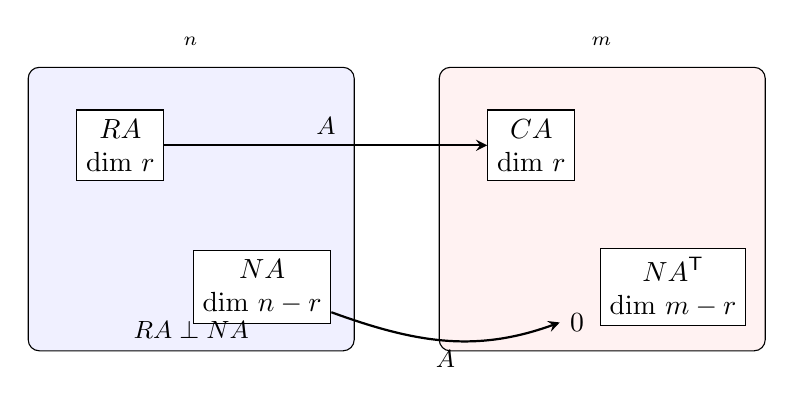
\begin{tikzpicture}[scale=0.9,>=stealth]
\draw[rounded corners,fill=blue!6] (-5.2,-1.8) rectangle (-0.6,2.2);
\node at (-2.9,2.5) {$\RR^n$};
\node[draw,fill=white,align=center] (R) at (-3.9,1.1) {$\rowsp{A}$\\dim $r$};
\node[draw,fill=white,align=center] (N) at (-1.9,-0.9) {$\nullsp{A}$\\dim $n-r$};
\draw[rounded corners,fill=red!5] (0.6,-1.8) rectangle (5.2,2.2);
\node at (2.9,2.5) {$\RR^m$};
\node[draw,fill=white,align=center] (C) at (1.9,1.1) {$\colsp{A}$\\dim $r$};
\node[draw,fill=white,align=center] (NT) at (3.9,-0.9) {$\nullsp{A\T}$\\dim $m-r$};
\draw[->,thick] (R) -- node[above,font=\small] {$A$} (C);
\draw[->,thick] (N) to[out=-20,in=-160] node[below,font=\small] {$A$} (2.3,-1.4) node[right] {$0$};
\node[font=\small] at (-2.9,-1.5) {$\rowsp{A}\perp\nullsp{A}$};
\node[font=\small] at (2.9,-1.5) {};
\end{tikzpicture}
\caption{The four fundamental subspaces. $A$ maps the row space one-to-one onto the column space and kills the null space.}
\label{fig:L14-four}
\end{figure}

\begin{theorem}\label{thm:L14-colspace}
For every $m\times n$ matrix $A$:
\begin{enumerate}
  \item $\nullsp{A}=\nullsp{A\T A}$;
  \item $\rank(A\T A)=\rank(A)$;
  \item $\colsp{A\T A}=\colsp{A\T}$.
\end{enumerate}
In particular, \cref{lem:L12-colspace} holds.
\end{theorem}
\begin{proof}
(1) If $x\in\nullsp{A}$, then $Ax=0$, so $A\T Ax=0$ and $x\in\nullsp{A\T A}$. Conversely, if $A\T Ax=0$, then
\[
0=x\T A\T Ax=\langle Ax,Ax\rangle=\pnorm{Ax}^2 ,
\]
so $Ax=0$ and $x\in\nullsp{A}$.
(2) $A$ and $A\T A$ both have $n$ columns. By rank--nullity and (1),
$\rank(A\T A)=n-\dim\nullsp{A\T A}=n-\dim\nullsp{A}=\rank(A)$.
(3) $\colsp{A\T A}\subseteq\colsp{A\T}$, because $A\T Ax=A\T(Ax)$. Both spaces have dimension $\rank(A\T A)=\rank(A)=\rank(A\T)$
by (2). A subspace contained in another of the same finite dimension equals it.
\end{proof}
\begin{note}
The notes add: ``in the recording it was mentioned $\colsp{A}$ instead of $\colsp{A\T}$''. The correct statement
is $\colsp{A\T A}=\colsp{A\T}$, a subspace of $\RR^n$. The spaces $\colsp{A\T A}$ and $\colsp{A}$ in general lie in
different spaces ($\RR^n$ versus $\RR^m$). Note also that $\colsp{AA\T}=\colsp{A}$, by the theorem applied to $A\T$.
\end{note}

\subsection{A formula for $\PX$}
\begin{proposition}[Supplementary: $\PX$ via a generalized inverse]\label{prop:L14-PXformula}
For any generalized inverse $\ginv{(X\T X)}$,
\[
\PX=X\ginv{(X\T X)}X\T ,
\]
and this matrix does not depend on the choice of generalized inverse. If $\rank X=p$, then $\PX=X(X\T X)^{-1}X\T$.
\end{proposition}
\begin{proof}
Let $G=\ginv{(X\T X)}$. By the note in \cref{sec:L12}, $\hat\beta=GX\T Y$ solves the normal equations for every $Y$. By
\cref{prop:L14-PX}, $XGX\T Y=X\hat\beta=\PX Y$ for all $Y$, so $XGX\T=\PX$. The right-hand side is the unique projection matrix, so it
does not depend on $G$.
\end{proof}

\begin{example}[$\PX$ in the one-way model]\label{ex:L14-PXoneway}
For \cref{ex:L12-oneway} ($k=2$, $n_1=n_2=2$), $\colsp{X}$ is spanned by the orthonormal vectors
$u_1=\frac1{\sqrt2}(1,1,0,0)\T$ and $u_2=\frac1{\sqrt2}(0,0,1,1)\T$. So
\[
\PX=u_1u_1\T+u_2u_2\T=\begin{pmatrix}\tfrac12&\tfrac12&0&0\\\tfrac12&\tfrac12&0&0\\0&0&\tfrac12&\tfrac12\\0&0&\tfrac12&\tfrac12\end{pmatrix},
\qquad \PX Y=\PX\begin{pmatrix}3\\5\\8\\10\end{pmatrix}=\begin{pmatrix}4\\4\\9\\9\end{pmatrix}=X\hat\beta(t)\ \ \forall t .
\]
$\tr\PX=2=\rank X$. The residual is $(I-\PX)Y=(-1,1,-1,1)\T$ and $R_0^2=4$. With $G=\mathrm{diag}(0,\tfrac12,\tfrac12)$
(\cref{prob:L12-4}), $XGX\T$ gives the same matrix.
\end{example}

\subsection{Computation}
\nb{week04/L14\_matrices\_projection.ipynb} computes the four subspaces of \cref{ex:L14-subspaces} with
\texttt{scipy.linalg.null\_space} and \texttt{orth}. It verifies $\nullsp{A}=\nullsp{A\T A}$ and the rank identities on random
rank-deficient matrices, builds $\PX$ in three ways (orthonormal basis, $X(X\T X)^{+}X\T$, $X\,\ginv{(X\T X)}X\T$ with a
hand-made $G$), and checks symmetry, idempotence and trace.

\subsection{Summary}
\begin{itemize}
  \item $X\beta$ is estimable, and its least squares estimate is $X\hat\beta=\PX Y$, the orthogonal projection of $Y$ onto $\colsp{X}$.
  \item $\PX=\sum u_iu_i\T=X\ginv{(X\T X)}X\T$: symmetric, idempotent, trace $=\rank X$.
  \item $\nullsp{A}=\nullsp{A\T A}$, $\rank A\T A=\rank A$, $\colsp{A\T A}=\colsp{A\T}$ (rank--nullity).
  \item $\rowsp{A}\perp\nullsp{A}$ in $\RR^n$ and $\colsp{A}\perp\nullsp{A\T}$ in $\RR^m$.
\end{itemize}

\subsection{Exercises}
\begin{problem}\label{prob:L14-1}
Show that $I-\PX$ is the orthogonal projection onto $\colsp{X}^\perp=\nullsp{X\T}$, and that $\PX(I-\PX)=0$.
\end{problem}
\begin{problem}\label{prob:L14-2}
Compute $\PX$ for simple linear regression with $x=(1,2,3,4)$ and verify that $\PX Y=(1.9,3.3,4.7,6.1)\T$ for $Y=(2,3,5,6)\T$.
\end{problem}
\begin{problem}\label{prob:L14-3}
For the one-way model with general $k$ and $n_i$, show that $\PX$ is block diagonal with blocks $\frac1{n_i}\one_{n_i}\one_{n_i}\T$, and that $(\PX Y)_{ij}=\bar Y_{i\cdot}$.
\end{problem}
\begin{problem}\label{prob:L14-4}
Find the four fundamental subspaces of $B=\begin{pmatrix}1&0&1\\0&1&1\end{pmatrix}$ and check rank--nullity.
\end{problem}
\begin{problem}\label{prob:L14-5}
Prove that if $P$ is symmetric and idempotent, then $P$ is the orthogonal projection onto $\colsp{P}$.
\end{problem}

\subsection{Further reading}
Christensen, Appendix~A (vector spaces), Appendix~B.3 (projections) and \S2.2; Rao, \S1a--1c (vector spaces,
matrices, projection operators) and \S4a.


\section*{Solutions to the Exercises of Chapter~\ref{ch:week04}}
\addcontentsline{toc}{section}{Solutions to the exercises}

\paragraph{\Cref{prob:L11-1}.}
With columns $(\mu,\alpha_1,\alpha_2,\beta_1,\beta_2,\beta_3)$ and cells ordered $(1,1)$, $(1,2)$, $(1,3)$, $(2,1)$, $(2,2)$, $(2,3)$:
\[
X=\begin{pmatrix}1&1&0&1&0&0\\1&1&0&0&1&0\\1&1&0&0&0&1\\1&0&1&1&0&0\\1&0&1&0&1&0\\1&0&1&0&0&1\end{pmatrix}.
\]
Column $\mu$ equals $\alpha_1+\alpha_2$ and also $\beta_1+\beta_2+\beta_3$, and by \cref{prop:L11-tworank} there is no
other relation. So $\rank X=6-2=4=I+J-1$.

\paragraph{\Cref{prob:L11-2}.}
The $\gamma_{22}$ column is zero. The non-zero cell indicators $g_{11},g_{12},g_{21}$ are independent, and all other
columns are sums of them ($\alpha_1=g_{11}+g_{12}$, $\alpha_2=g_{21}$, $\beta_1=g_{11}+g_{21}$, $\beta_2=g_{12}$). So
$\rank X=3$, the number of non-empty cells.

\paragraph{\Cref{prob:L11-3}.}
The row of $X$ for any observation in subgroup $(i,j)$ is $\lambda=e_\mu+e_{\mu_i}+e_{\delta_{ij}}$, so
$\mu+\mu_i+\delta_{ij}=\EE[Y_{ijl}]$ is estimable. Linear unbiased estimates include $Y_{ij1}$ and, better,
$\bar Y_{ij\cdot}=\frac1{n_{ij}}\sum_lY_{ijl}$.

\paragraph{\Cref{prob:L11-4}.}
The rows for cells $(1,j)$ and $(2,j)$ are $e_\mu+e_{\alpha_1}+e_{\beta_j}$ and $e_\mu+e_{\alpha_2}+e_{\beta_j}$. Their difference
is $e_{\alpha_1}-e_{\alpha_2}\in\colsp{X\T}$, so $\alpha_1-\alpha_2$ is estimable, for instance by $Y_{1j1}-Y_{2j1}$.

\paragraph{\Cref{prob:L12-1}.}
$X\T X=\begin{pmatrix}n&\sum x_i\\\sum x_i&\sum x_i^2\end{pmatrix}$ and $X\T Y=\begin{pmatrix}\sum Y_i\\\sum x_iY_i\end{pmatrix}$.
The first equation, $n\beta_1+\beta_2\sum x_i=\sum Y_i$, gives $\beta_1=\bar Y-\beta_2\bar x$. Substituting into
the second: $\beta_2(\sum x_i^2-n\bar x^2)=\sum x_iY_i-n\bar x\bar Y$, i.e.\ $\beta_2S_{xx}=S_{xY}$, which is
\cref{thm:L05-slr}.

\paragraph{\Cref{prob:L12-2}.}
$(X\T Y)_\mu=\sum_{i,j}Y_{ij}$ and $(X\T Y)_{\mu_i}=\sum_jY_{ij}=n_i\bar Y_{i\cdot}$. $(X\T X\beta)_{\mu_i}=n_i(\mu+\mu_i)$, and
$(X\T X\beta)_\mu=\sum_in_i(\mu+\mu_i)$. The $\mu_i$-equations say $\mu+\mu_i=\bar Y_{i\cdot}$. The $\mu$-equation is their
weighted sum, so it adds nothing. Then $X\hat\beta$ has entry $\bar Y_{i\cdot}$ in every row of group $i$, and
$R_0^2=\sum_{i,j}(Y_{ij}-\bar Y_{i\cdot})^2=\SSW$.

\paragraph{\Cref{prob:L12-3}.}
If $\one=Xc$, then $\one\T\hat e=c\T X\T\hat e=0$ by the normal equations.

\paragraph{\Cref{prob:L12-4}.}
$X\T XG=\begin{pmatrix}0&1&1\\0&1&0\\0&0&1\end{pmatrix}$, and multiplying by $X\T X$ gives back
$\begin{pmatrix}4&2&2\\2&2&0\\2&0&2\end{pmatrix}$. So $G$ is a generalized inverse. $GX\T Y=(0,\,8/2,\,18/2)\T=(0,4,9)\T$, which is
the solution with $t=0$.

\paragraph{\Cref{prob:L13-1}.}
By \cref{prob:L12-2} every solution has $\hat\mu+\hat\mu_i=\bar Y_{i\cdot}$. Hence
$\sum c_i\hat\mu_i=\sum c_i(\bar Y_{i\cdot}-\hat\mu)=\sum c_i\bar Y_{i\cdot}-\hat\mu\sum c_i=\sum c_i\bar Y_{i\cdot}$.

\paragraph{\Cref{prob:L13-2}.}
Write $\lambda=X\T Xb$. Then $\lambda\T\hat\beta=b\T X\T Y$ and
$\Var(\lambda\T\hat\beta)=\sigma^2b\T X\T Xb$ (\cref{prop:L09-rules}). For any generalized inverse $G$,
$\lambda\T G\lambda=b\T X\T X\,G\,X\T Xb=b\T X\T Xb$. So $\Var(\lambda\T\hat\beta)=\sigma^2\lambda\T G\lambda$, whatever $G$ is.

\paragraph{\Cref{prob:L13-3}.}
$X=[\one,x,2x]$ has $\colsp{X}=\colsp{[\one,x]}$, so the fitted values are those of \cref{ex:L12-slr}. The normal equations
reduce to $\beta_1=0.5$ and $\beta_2+2\beta_3=1.4$. All solutions are $(0.5,\ 1.4-2s,\ s)\T$, $s\in\RR$. The
estimate of the estimable function $\beta_2+2\beta_3$ is $1.4$ for every $s$.

\paragraph{\Cref{prob:L13-4}.}
Take $X=[x,x,x]$ with $x=(1,2)\T$. Then $\nullsp{X}=\{v:v_1+v_2+v_3=0\}$ is two-dimensional. For
$\lambda=(1,0,0)\T$ (not estimable, since $\lambda\T(1,-1,0)\T\ne0$), the two solutions $\hat\beta$ and $\hat\beta+(0,1,-1)\T$ give
the same $\lambda\T\hat\beta$. This does not contradict the theorem, which requires equality for \emph{all} solutions, i.e.\
$\lambda\perp$ \emph{every} $v\in\nullsp{X}$.

\paragraph{\Cref{prob:L14-1}.}
$I-\PX$ is symmetric, and $(I-\PX)^2=I-2\PX+\PX^2=I-\PX$. For $y$, $(I-\PX)y=y-\PX y\perp\colsp{X}$. Also
$y-(I-\PX)y=\PX y\in\colsp{X}$, which is orthogonal to $\colsp{X}^\perp$. By uniqueness in \cref{lem:L14-projection},
$I-\PX$ projects onto $\colsp{X}^\perp$. This space equals $\nullsp{X\T}$, because $X\T z=0$ iff $z$ is orthogonal to every
column. Finally $\PX(I-\PX)=\PX-\PX^2=0$.

\paragraph{\Cref{prob:L14-2}.}
$(X\T X)^{-1}=\frac1{20}\begin{pmatrix}30&-10\\-10&4\end{pmatrix}$, so $(\PX)_{ij}=\frac1{20}(30-10(x_i+x_j)+4x_ix_j)$:
\[
\PX=\begin{pmatrix}0.7&0.4&0.1&-0.2\\0.4&0.3&0.2&0.1\\0.1&0.2&0.3&0.4\\-0.2&0.1&0.4&0.7\end{pmatrix},
\qquad \PX(2,3,5,6)\T=(1.9,3.3,4.7,6.1)\T .
\]
The trace is $0.7+0.3+0.3+0.7=2=\rank X$.

\paragraph{\Cref{prob:L14-3}.}
The normalised group indicators $u_i=\one_{(i)}/\sqrt{n_i}$ form an orthonormal basis of $\colsp{X}$, where $\one_{(i)}$ is the
indicator of group $i$. They are orthogonal because their supports are disjoint. Hence
$\PX=\sum_i\frac1{n_i}\one_{(i)}\one_{(i)}\T$, which is block diagonal with blocks $\frac1{n_i}\one\one\T$. Then
$(\PX Y)_{ij}=\frac1{n_i}\sum_lY_{il}=\bar Y_{i\cdot}$.

\paragraph{\Cref{prob:L14-4}.}
$\rank B=2$, so $\colsp{B}=\RR^2$ and $\nullsp{B\T}=\{0\}$. $\rowsp{B}=\mathrm{span}\{(1,0,1)\T,(0,1,1)\T\}$ and
$\nullsp{B}=\mathrm{span}\{(1,1,-1)\T\}$, which is orthogonal to both rows. Rank--nullity: $2+1=3$.

\paragraph{\Cref{prob:L14-5}.}
For $y\in\RR^n$, $Py\in\colsp{P}$. For any $v=Pz\in\colsp{P}$,
$\langle y-Py,Pz\rangle=z\T P\T(y-Py)=z\T(Py-P^2y)=0$. So $y-Py\perp\colsp{P}$, and $Py$ is the orthogonal projection
(\cref{def:L14-proj}).

% ============================================================
% Week 5 -- Estimation, inference and assessment in simple linear regression
% ============================================================
\chapter{Inference for Linear Models and Computation in R}\label{ch:week05}

This chapter covers Week~5 (Lectures 15--18). \textbf{Source caveat.} The instructor's Week-5 lecture notes
(\texttt{Feb21.pdf}) were \emph{not} accessed. The chapter is built from the Week-5 R code (\texttt{Feb21.r}), the
Week-5 assignment (\texttt{hw56.pdf}), and the standard theory that the code and assignment use. The theory is written
in the notation of the earlier chapters. Every numerical value shown was reproduced in the companion notebooks.

% ============================================================
% Lecture 15 -- Estimating the coefficients of linear models
% ============================================================
\section{Estimating the Coefficients of Linear Models}\label{sec:L15}

\lectureheader{15}{qF9VBw3CP78}{Week-5 R code \texttt{Feb21.r} (least squares fit of \texttt{iris}, normal equations by hand) and Week-5 assignment Q4. The Week-5 lecture PDF was \emph{not} accessed. The derivations below follow the titles and code and are marked accordingly.}

\begin{guiding*}
By the end of this lecture you should be able to:
\begin{itemize}
  \item compute $\hat\beta=(X\T X)^{-1}X\T Y$ for a full-rank model, by hand and in code;
  \item prove that $\hat\beta$ is unbiased with $\Cov(\hat\beta)=\sigma^2(X\T X)^{-1}$;
  \item derive $\Var(\hat\beta_0)$, $\Var(\hat\beta_1)$ and $\Cov(\hat\beta_0,\hat\beta_1)$ in simple linear regression;
  \item fit and plot a regression line with \texttt{lm}/\texttt{statsmodels}.
\end{itemize}
\end{guiding*}

\subsection{Recap}
Week~4 established that least squares estimates are the solutions of the normal equations
$X\T X\beta=X\T Y$ (\cref{thm:L12-normal}). The solution is unique iff $\rank X=p$
(\cref{cor:L12-fitted}), and $X\hat\beta=\PX Y$ (\cref{prop:L14-PX}). Week~5 applies this theory to
regression models, which in practice almost always have a full-rank $X$. Throughout this chapter we
write simple linear regression as
\[
Y_i=\beta_0+\beta_1x_i+\eps_i,\qquad i=1,\dots,n,
\]
the notation of the R output (``\texttt{(Intercept)}'' and the slope). In Week~2 we called these
coefficients $a_1,a_2$.

\subsection{The iris example from the R code}
\begin{example}[Sepal length on petal width]\label{ex:L15-iris}
The R code fits \texttt{lm(Sepal.Length \textasciitilde\ Petal.Width, data = iris)} to Fisher's iris data
($n=150$ flowers), plots the points, and adds the fitted line with \texttt{abline} and with
\texttt{ggplot(...) + stat\_smooth(method = "lm")}. The estimates are
\[
\hat\beta_0=4.7776,\qquad \hat\beta_1=0.8886 .
\]
A flower whose petals are $1$\,cm wider has, on average, sepals $0.89$\,cm longer. The line
passes through $(\bar x,\bar y)=(1.1993,\,5.8433)$ (\cref{cor:L05-props}).
\end{example}

\begin{figure}[ht]
\centering
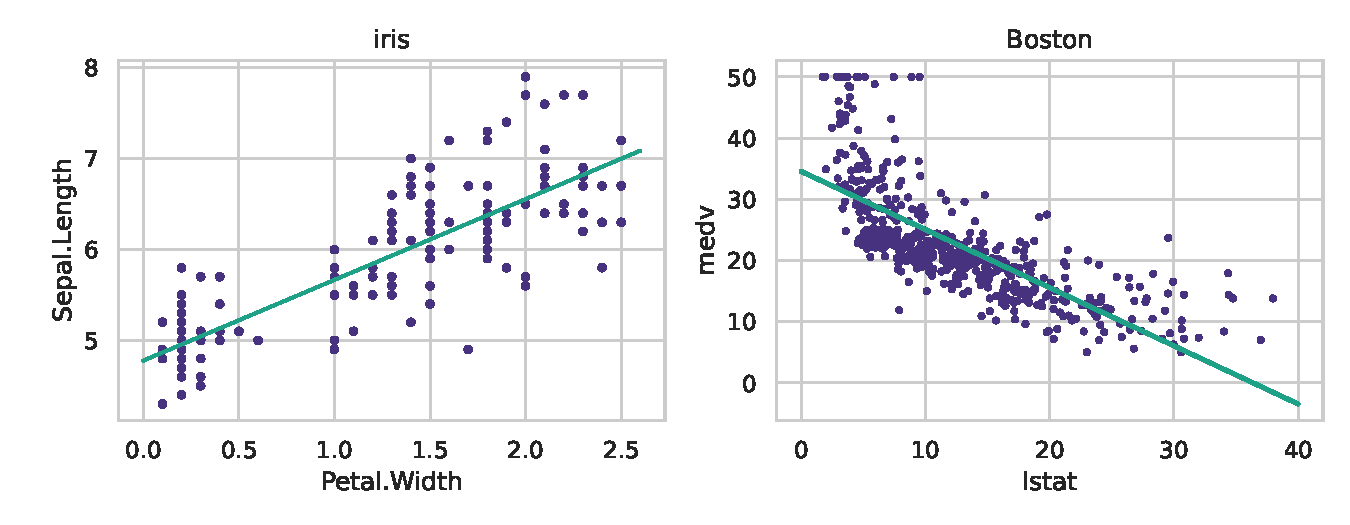
\includegraphics[width=0.95\textwidth]{figures/L15_iris_boston.pdf}
\caption{Least squares lines for \texttt{iris} (\cref{ex:L15-iris}) and for \texttt{Boston} (\cref{sec:L16}).}
\label{fig:L15-fits}
\end{figure}

\subsection{Normal equations by hand}
The second part of the R code solves the normal equations directly for a model with two
explanatory variables:
\begin{center}
\begin{minipage}{0.85\textwidth}\small\ttfamily
x1 <- c(10,0,45,56,79); x2 <- c(2,34,15,5,4)\\
y <- x1 + x2 + rnorm(5, mean=0, sd=0.3)\\
X <- as.matrix(cbind(1,x1,x2))\\
betahat = solve(t(X) \%*\% X) \%*\% (t(X) \%*\% Y) \quad \# solution of X\textasciicircum TX beta = X\textasciicircum Ty\\
lm.fit <- lm(y \textasciitilde\ 1+x1+x2); lm.fit\$coefficients
\end{minipage}
\end{center}
The data are simulated from $Y_i=0+1\cdot x_{1i}+1\cdot x_{2i}+\eps_i$ with $\sigma=0.3$, so $\hat\beta$ should be
close to $(0,1,1)$. Here $n=5$, $p=3$, and
\[
X\T X=\begin{pmatrix}5&190&60\\190&11502&1291\\60&1291&1426\end{pmatrix}.
\]
Its determinant is non-zero ($\rank X=3$), so \texttt{solve} works. The two computations agree. The
exact numbers depend on the random draw. With the notebook's seed they are
$\hat\beta=(0.3665,\ 0.9905,\ 1.0068)$. Different runs of the R code give different numbers, because the
original code sets no seed.

\subsection[Unbiasedness and covariance of the estimator]{Unbiasedness and covariance of \texorpdfstring{$\protect\hat\beta$}{beta-hat}}
\begin{theorem}\label{thm:L15-moments}
Let $(Y,X\beta,\sigma^2I_n)$ be a linear model with $\rank X=p$, and let $\hat\beta=(X\T X)^{-1}X\T Y$. Then
\[
\EE[\hat\beta]=\beta,\qquad \Cov(\hat\beta)=\sigma^2(X\T X)^{-1}.
\]
\end{theorem}
\begin{proof}
$\hat\beta=AY$ with the fixed matrix $A=(X\T X)^{-1}X\T$. By \cref{prop:L09-rules},
$\EE\hat\beta=A\,X\beta=(X\T X)^{-1}X\T X\beta=\beta$. Also
\[
\Cov(\hat\beta)=A(\sigma^2I)A\T=\sigma^2(X\T X)^{-1}X\T X(X\T X)^{-1}=\sigma^2(X\T X)^{-1},
\]
using the symmetry of $(X\T X)^{-1}$.
\end{proof}

\begin{corollary}[Simple linear regression; Week-5 assignment Q4]\label{cor:L15-slr}
For $Y_i=\beta_0+\beta_1x_i+\eps_i$ with the $x_i$ not all equal,
\[
X\T X=\begin{pmatrix}n&\sum x_i\\\sum x_i&\sum x_i^2\end{pmatrix},\qquad X\T Y=\begin{pmatrix}\sum Y_i\\\sum x_iY_i\end{pmatrix},
\]
$\hat\beta_1=S_{xY}/S_{xx}$, $\hat\beta_0=\bar Y-\hat\beta_1\bar x$, and
\[
\Var(\hat\beta_1)=\frac{\sigma^2}{S_{xx}},\qquad
\Var(\hat\beta_0)=\sigma^2\Bigl(\frac1n+\frac{\bar x^2}{S_{xx}}\Bigr),\qquad
\Cov(\hat\beta_0,\hat\beta_1)=-\frac{\sigma^2\bar x}{S_{xx}} .
\]
\end{corollary}
\begin{proof}
The formulas for $X\T X$, $X\T Y$ and $\hat\beta$ are \cref{prob:L12-1}. Now $\det(X\T X)=n\sum x_i^2-(\sum x_i)^2=nS_{xx}$, so
\[
(X\T X)^{-1}=\frac1{nS_{xx}}\begin{pmatrix}\sum x_i^2&-\sum x_i\\-\sum x_i&n\end{pmatrix}.
\]
By \cref{thm:L15-moments}: $\Var(\hat\beta_1)=\sigma^2 n/(nS_{xx})=\sigma^2/S_{xx}$ and
$\Cov(\hat\beta_0,\hat\beta_1)=-\sigma^2 n\bar x/(nS_{xx})=-\sigma^2\bar x/S_{xx}$. For the intercept,
$\Var(\hat\beta_0)=\sigma^2\sum x_i^2/(nS_{xx})$, and $\sum x_i^2=S_{xx}+n\bar x^2$ gives
$\sigma^2(1/n+\bar x^2/S_{xx})$.

A direct check without matrices: $\hat\beta_1=\sum_i c_iY_i$ with $c_i=(x_i-\bar x)/S_{xx}$, so
$\Var(\hat\beta_1)=\sigma^2\sum c_i^2=\sigma^2S_{xx}/S_{xx}^2$. Also $\Cov(\bar Y,\hat\beta_1)=\frac{\sigma^2}{n}\sum c_i=0$.
Then $\Var(\hat\beta_0)=\Var(\bar Y)+\bar x^2\Var(\hat\beta_1)-2\bar x\Cov(\bar Y,\hat\beta_1)$, which gives the same result.
\end{proof}

\begin{example}[The hand example again]\label{ex:L15-hand}
For $x=(1,2,3,4)$ (\cref{ex:L12-slr}): $n=4$, $\bar x=2.5$, $S_{xx}=5$, and
\[
(X\T X)^{-1}=\frac1{20}\begin{pmatrix}30&-10\\-10&4\end{pmatrix}=\begin{pmatrix}1.5&-0.5\\-0.5&0.2\end{pmatrix}.
\]
So $\Var(\hat\beta_1)=0.2\sigma^2=\sigma^2/5$, $\Var(\hat\beta_0)=1.5\sigma^2=\sigma^2(1/4+6.25/5)$ and
$\Cov(\hat\beta_0,\hat\beta_1)=-0.5\sigma^2=-2.5\sigma^2/5$, in agreement with \cref{cor:L15-slr}. The
correlation of the two estimates is $-0.5/\sqrt{1.5\times0.2}=-0.913$. Because all $x_i>0$, overestimating the
slope goes with underestimating the intercept.
\end{example}

\begin{note}[Supplementary: design matters]
$\Var(\hat\beta_1)=\sigma^2/S_{xx}$ is small when the $x_i$ are spread out. To estimate a slope well, take
observations far apart. $\Var(\hat\beta_0)$ is smallest when $\bar x=0$. Centring the covariate ($x_i-\bar x$)
makes $\hat\beta_0=\bar Y$ and the two estimates uncorrelated.
\end{note}

\subsection{Computation}
\begin{center}\small
\begin{tabular}{@{}>{\raggedright\arraybackslash}p{7cm}>{\raggedright\arraybackslash}p{8.4cm}@{}}\hline
R & Python\\\hline
\texttt{lm(Sepal.Length \textasciitilde\ Petal.Width, iris)} & \texttt{smf.ols("Sepal\_Length \textasciitilde\ Petal\_Width", ir).fit()}\\
\texttt{abline(fit1)} & \texttt{ax.plot(xs, b0 + b1*xs)}\\
\texttt{stat\_smooth(method="lm")} & \texttt{sns.regplot(...)}\\
\texttt{solve(t(X)\%*\%X) \%*\% t(X)\%*\%Y} & \texttt{np.linalg.solve(X.T @ X, X.T @ Y)}\\
\texttt{vcov(fit)} & \texttt{fit.cov\_params()}\\\hline
\end{tabular}
\end{center}
\nb{week05/L15\_estimating\_coefficients.ipynb} also checks $\Cov(\hat\beta)=\sigma^2(X\T X)^{-1}$ by simulation.

\subsection{Summary}
\begin{itemize}
  \item Full rank: $\hat\beta=(X\T X)^{-1}X\T Y$, $\EE\hat\beta=\beta$, $\Cov\hat\beta=\sigma^2(X\T X)^{-1}$.
  \item SLR: $\Var\hat\beta_1=\sigma^2/S_{xx}$, $\Var\hat\beta_0=\sigma^2(1/n+\bar x^2/S_{xx})$, $\Cov=-\sigma^2\bar x/S_{xx}$.
  \item \texttt{iris}: $\widehat{\text{Sepal.Length}}=4.7776+0.8886\,\text{Petal.Width}$.
\end{itemize}

\subsection{Exercises}
\begin{problem}\label{prob:L15-1}
Show that $\hat\beta_1=\sum_ic_iY_i$ with $c_i=(x_i-\bar x)/S_{xx}$, and that $\sum c_i=0$, $\sum c_ix_i=1$.
\end{problem}
\begin{problem}\label{prob:L15-2}
For $x=(-1,0,1)$, compute $\Cov(\hat\beta)$ in simple linear regression. Why are $\hat\beta_0$ and $\hat\beta_1$ uncorrelated here?
\end{problem}
\begin{problem}\label{prob:L15-3}
Show that $\Var(\hat\beta_0+\hat\beta_1x_0)=\sigma^2\bigl(\frac1n+\frac{(x_0-\bar x)^2}{S_{xx}}\bigr)$.
\end{problem}
\begin{problem}\label{prob:L15-4}
You may choose $n=10$ design points $x_i\in[0,1]$. Which choice minimises $\Var(\hat\beta_1)$?
\end{problem}

\subsection{Further reading}
Christensen, \S2.2 and Chapter~6 (simple linear regression); Rao, \S4a.2; James, Witten, Hastie
\& Tibshirani, \emph{An Introduction to Statistical Learning}, \S3.1 (the source of the lab in the R code).

% ============================================================
% Lecture 16 -- Interval estimates and hypothesis tests for coefficients
% ============================================================
\section{Interval Estimates and Hypothesis Tests for the Coefficients}\label{sec:L16}

\lectureheader{16}{dXYKDrO7vE8}{Week-5 R code \texttt{Feb21.r} (Boston lab: \texttt{summary}, \texttt{confint}; $t$-distribution functions \texttt{pt}, \texttt{qt}). The Week-5 lecture PDF was \emph{not} accessed. The theory is filled in from the course's own framework.}

\begin{guiding*}
By the end of this lecture you should be able to:
\begin{itemize}
  \item show that $\RSS/(n-r)$ is an unbiased estimate of $\sigma^2$;
  \item under normal errors, derive the distribution of $(\hat\beta_j-\beta_j)/\widehat{\mathrm{SE}}(\hat\beta_j)$;
  \item construct confidence intervals for regression coefficients and test $H_0:\beta_j=0$;
  \item read the coefficient table of \texttt{summary(lm(...))}.
\end{itemize}
\end{guiding*}

\subsection{Recap}
$\hat\beta$ is unbiased with $\Cov\hat\beta=\sigma^2(X\T X)^{-1}$ (\cref{thm:L15-moments}). To turn this into
confidence intervals and tests we need two more things: an estimate of the unknown $\sigma^2$, and the
exact distribution of the estimates. The latter requires the normality assumption, which also
underlies \cref{thm:L08-dist}.

\subsection{Estimating $\sigma^2$}
\begin{theorem}\label{thm:L16-s2}
In the linear model $(Y,X\beta,\sigma^2I_n)$ with $\rank X=r<n$, the residual sum of squares
$\RSS=\pnorm{Y-X\hat\beta}^2=\pnorm{(I-\PX)Y}^2$ satisfies $\EE[\RSS]=(n-r)\sigma^2$. Hence
\[
s^2=\frac{\RSS}{n-r}
\]
is an unbiased estimate of $\sigma^2$.
\end{theorem}
\begin{proof}
Let $M=I-\PX$. It is symmetric and idempotent (\cref{prob:L14-1}), so $\RSS=Y\T M\T MY=Y\T MY$. Since
$MX=X-\PX X=0$ (every column of $X$ lies in $\colsp{X}$), we get $MY=M(X\beta+\eps)=M\eps$ and $\RSS=\eps\T M\eps$. For any fixed matrix $M$,
\[
\EE[\eps\T M\eps]=\EE\Bigl[\sum_{i,l}M_{il}\eps_i\eps_l\Bigr]=\sum_{i,l}M_{il}\,\sigma^2\mathbbm 1\{i=l\}=\sigma^2\tr M ,
\]
using $\EE[\eps_i\eps_l]=\sigma^2$ if $i=l$ and $0$ otherwise. Finally
$\tr M=n-\tr\PX=n-r$ (\cref{lem:L14-projection}).
\end{proof}
In simple linear regression $r=2$ and $s^2=\RSS/(n-2)$. Its square root is the \emph{residual standard
error} of \cref{sec:L17}. For the one-way model $r=k$ and $s^2=\SSW/(n-k)$ (\cref{prob:L08-1}).

\subsection{Distributions under normality}
\begin{theorem}[Sampling distribution of $\hat\beta$]\label{thm:L16-dist}
Assume $\eps\sim\N(0,\sigma^2I_n)$ and $\rank X=p<n$. Then
\begin{enumerate}
  \item $\hat\beta\sim\N\bigl(\beta,\sigma^2(X\T X)^{-1}\bigr)$;
  \item $\RSS/\sigma^2\sim\chi^2_{n-p}$;
  \item $\hat\beta$ and $\RSS$ are independent;
  \item for each $j$, with $v_{jj}=[(X\T X)^{-1}]_{jj}$ and $\widehat{\mathrm{SE}}(\hat\beta_j)=s\sqrt{v_{jj}}$,
  \[
  T_j=\frac{\hat\beta_j-\beta_j}{\widehat{\mathrm{SE}}(\hat\beta_j)}\sim t_{n-p}.
  \]
\end{enumerate}
\end{theorem}
\begin{proof}
(1) $\hat\beta=(X\T X)^{-1}X\T Y$ is a linear function of the normal vector $Y$, so it is normal. Its mean and
covariance are given by \cref{thm:L15-moments}.
(2) As in the proof of \cref{thm:L16-s2}, $\RSS/\sigma^2=Z\T MZ$ with $Z=\eps/\sigma\sim\N(0,I_n)$ and $M=I-\PX$
symmetric idempotent of rank $n-p$. \Cref{lem:L08-chisq} gives $\chi^2_{n-p}$.
(3) $\hat\beta$ is a function of $U=X\T Y$, and $\RSS=\pnorm{MY}^2$ is a function of $V=MY$. The pair $(U,V)$ is jointly normal,
and $\Cov(X\T Y,MY)=X\T(\sigma^2I)M\T=\sigma^2(MX)\T=0$. By \cref{lem:L08-indep}, $U\indep V$, so $\hat\beta\indep\RSS$.
(4) $Z_j=(\hat\beta_j-\beta_j)/(\sigma\sqrt{v_{jj}})\sim\N(0,1)$ by (1). Also $W=\RSS/\sigma^2\sim\chi^2_{n-p}$ by (2), and $Z_j\indep W$ by (3).
Then $T_j=Z_j/\sqrt{W/(n-p)}$, which is the definition of the $t_{n-p}$ distribution. The unknown $\sigma$ cancels.
\end{proof}

\begin{corollary}[Confidence interval and $t$-test]\label{cor:L16-ci}
Let $t_{n-p,\,1-\alpha/2}$ be the $(1-\alpha/2)$-quantile of $t_{n-p}$ (R: \texttt{qt(1-alpha/2, df)}).
\begin{enumerate}
  \item $\hat\beta_j\pm t_{n-p,\,1-\alpha/2}\,\widehat{\mathrm{SE}}(\hat\beta_j)$ is a $100(1-\alpha)\%$ confidence interval for $\beta_j$.
  \item To test $H_0:\beta_j=b$ against $H_1:\beta_j\ne b$, use $t=(\hat\beta_j-b)/\widehat{\mathrm{SE}}(\hat\beta_j)$. Reject at level $\alpha$ if $\abs t>t_{n-p,1-\alpha/2}$. The p-value is $2\,\PP(T>\abs t)$ for $T\sim t_{n-p}$ (R: \texttt{2*(1-pt(abs(t), df))}).
\end{enumerate}
\end{corollary}
\begin{proof}
(1) $\PP\bigl(\abs{T_j}\le t_{n-p,1-\alpha/2}\bigr)=1-\alpha$ by symmetry of the $t$ distribution. Rearranging the inequality
$\abs{\hat\beta_j-\beta_j}\le t_{n-p,1-\alpha/2}\widehat{\mathrm{SE}}$ gives the interval.
(2) Under $H_0$, $t\sim t_{n-p}$, so $\PP_{H_0}(\abs t>t_{n-p,1-\alpha/2})=\alpha$.
\end{proof}

\begin{example}[By hand: the four-point data]\label{ex:L16-hand}
$x=(1,2,3,4)$, $Y=(2,3,5,6)$, with $\hat\beta=(0.5,1.4)$ and $\RSS=0.2$ (\cref{ex:L05-hand}). Here $n-p=2$.
\begin{itemize}
  \item $s^2=0.2/2=0.1$ and $s=0.3162$.
  \item $\widehat{\mathrm{SE}}(\hat\beta_1)=\sqrt{0.1\times 0.2}=\sqrt{0.02}=0.14142$ and $\widehat{\mathrm{SE}}(\hat\beta_0)=\sqrt{0.1\times1.5}=0.38730$ (\cref{ex:L15-hand}).
  \item $t$ for $H_0:\beta_1=0$: $1.4/0.14142=9.8995$. With $2$ degrees of freedom the p-value is $2\PP(T>9.8995)=0.01005$, so we reject at $5\%$ but not at $1\%$.
  \item $t_{2,0.975}=4.3027$. The $95\%$ interval for $\beta_1$ is $1.4\pm4.3027\times0.14142=1.4\pm0.6085=(0.7915,\,2.0085)$.
  \item Intercept: $t=0.5/0.3873=1.291$ with p-value $0.326$. Its $95\%$ interval is $0.5\pm1.6664=(-1.1664,\,2.1664)$, which contains $0$.
\end{itemize}
With only $2$ degrees of freedom, the quantile $4.30$ is far larger than the normal $1.96$.
\end{example}

\subsection{The Boston example from the R code}
\begin{example}[\texttt{medv} on \texttt{lstat}]\label{ex:L16-boston}
The code follows the lab of Chapter~3 of \emph{An Introduction to Statistical Learning}. \texttt{Boston} has
$n=506$ census tracts. \texttt{medv} is the median house value (in \$1000s), and \texttt{lstat} is the
percentage of lower-status population. The first call, \texttt{lm(medv \textasciitilde\ lstat)}, gives an error
because \texttt{Boston} was not specified as the data. The fix is \texttt{data = Boston}, or \texttt{attach(Boston)}.
\texttt{summary(lm.fit)} prints
\begin{center}
\begin{tabular}{lrrrr}\hline
 & Estimate & Std.\ Error & $t$ value & $\PP(>\abs t)$\\\hline
(Intercept) & $34.5538$ & $0.5626$ & $61.415$ & $<2\times10^{-16}$\\
lstat & $-0.9500$ & $0.0387$ & $-24.528$ & $<2\times10^{-16}$\\\hline
\end{tabular}
\end{center}
on $504$ degrees of freedom. \texttt{confint(lm.fit)} gives the $95\%$ intervals
\[
\beta_0\in(33.4485,\ 35.6592),\qquad \beta_1\in(-1.0261,\ -0.8740),
\]
i.e.\ $\hat\beta_j\pm1.9647\,\widehat{\mathrm{SE}}$, where $t_{504,0.975}=1.9647$. Each additional percentage point of
lower-status population is associated with a decrease of between \$874 and \$1026 in median value. The
relationship is overwhelmingly significant. (The residual plot in \cref{sec:L18} shows that it is also
not linear.)
\end{example}

\subsection{The $t$ distribution in R}
The last part of the R code explores the $t$ distribution.
\begin{itemize}
  \item \texttt{1 - pt(1:5, df = 1)} gives the upper-tail probabilities $0.25000, 0.14758, 0.10242, 0.07798, 0.06283$. The Cauchy ($t_1$) tails are very heavy.
  \item \texttt{qt(.975, df = c(1:10,20,50,100,1000))} gives $12.706, 4.303, 3.182, 2.776, 2.571,\dots,2.228$ ($df=10$), $2.086$ ($20$), $2.009$ ($50$), $1.984$ ($100$) and $1.962$ ($1000$). As the degrees of freedom grow, the quantiles decrease to the normal value $1.960$.
  \item The non-central $t$ distribution (\texttt{pt(t, df=3, ncp=d)}, drawn with \texttt{image}/\texttt{persp}) is the distribution of $T_j$ when $H_0$ is \emph{false}. It determines the power of the $t$-test.
\end{itemize}

\begin{figure}[ht]
\centering
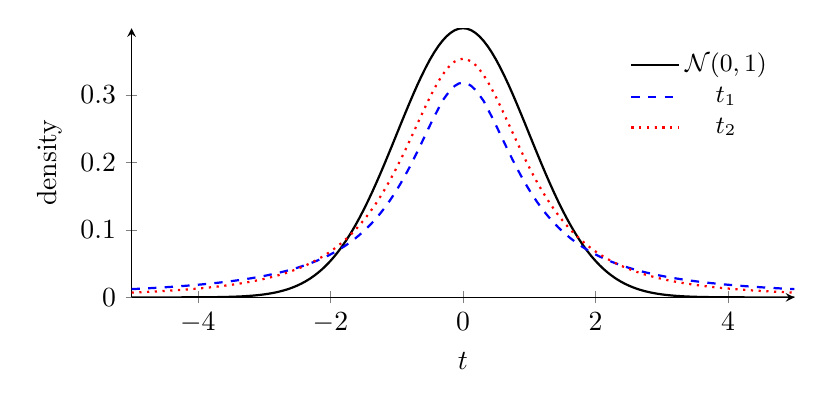
\begin{tikzpicture}
\begin{axis}[width=10cm,height=5cm,domain=-5:5,samples=161,axis lines=left,xlabel={$t$},ylabel={density},
  legend style={font=\small,draw=none,at={(0.98,0.95)},anchor=north east}]
\addplot[thick,black] {exp(-x^2/2)/sqrt(2*pi)};
\addplot[thick,blue,dashed] {1/(pi*(1+x^2))};
\addplot[thick,red,dotted] {0.3536*(1+x^2/2)^(-1.5)};
\legend{{$\N(0,1)$},{$t_1$},{$t_2$}}
\end{axis}
\end{tikzpicture}
\caption{The $t$ densities have heavier tails than the normal. This is why the critical values exceed $1.96$ when the degrees of freedom are small.}
\label{fig:L16-t}
\end{figure}

\subsection{Computation}
\begin{center}\small
\begin{tabular}{@{}>{\raggedright\arraybackslash}p{6.5cm}>{\raggedright\arraybackslash}p{8.9cm}@{}}\hline
R & Python\\\hline
\texttt{summary(lm.fit)} & \texttt{fit.summary()} (or \texttt{fit.params}, \texttt{fit.bse}, \texttt{fit.tvalues}, \texttt{fit.pvalues})\\
\texttt{confint(lm.fit)} & \texttt{fit.conf\_int()}\\
\texttt{pt(q, df)}, \texttt{qt(p, df)} & \texttt{scipy.stats.t.cdf(q, df)}, \texttt{stats.t.ppf(p, df)}\\
\texttt{pt(t, df, ncp)} & \texttt{stats.nct.cdf(t, df, ncp)}\\\hline
\end{tabular}
\end{center}
\nb{week05/L16\_intervals\_tests.ipynb} computes the coefficient table from the formulas, checks it against
\texttt{statsmodels}, and verifies the $95\%$ coverage and the $t_{n-p}$ distribution by simulation.

\subsection{Summary}
\begin{itemize}
  \item $s^2=\RSS/(n-r)$ is unbiased for $\sigma^2$, because $\EE[\eps\T M\eps]=\sigma^2\tr M$.
  \item Under normality: $\hat\beta\sim\N(\beta,\sigma^2(X\T X)^{-1})$, $\RSS/\sigma^2\sim\chi^2_{n-p}$, and they are independent. So $(\hat\beta_j-\beta_j)/\widehat{\mathrm{SE}}\sim t_{n-p}$.
  \item CI: $\hat\beta_j\pm t_{n-p,1-\alpha/2}\widehat{\mathrm{SE}}$. Test of $\beta_j=0$: $t=\hat\beta_j/\widehat{\mathrm{SE}}$.
  \item Boston: $\hat\beta_1=-0.9500$ (SE $0.0387$), CI $(-1.0261,-0.8740)$.
\end{itemize}

\subsection{Exercises}
\begin{problem}\label{prob:L16-1}
For the snowfall data of \cref{ex:L07-snow}, test $H_0:\beta_1=0$ at the $5\%$ level and give a $95\%$ CI for the slope.
\end{problem}
\begin{problem}\label{prob:L16-2}
Show that in simple linear regression the $t$ statistic for $\beta_1=0$ can be written $t=r\sqrt{n-2}/\sqrt{1-r^2}$, where $r$ is the sample correlation.
\end{problem}
\begin{problem}\label{prob:L16-3}
Why can we not use $\RSS/n$ in place of $s^2$ in \cref{thm:L16-dist}(4)? What is $\EE[\RSS/n]$?
\end{problem}
\begin{problem}\label{prob:L16-4}
In \cref{ex:L16-hand}, test $H_0:\beta_1=1$ against $\beta_1\ne 1$ at the $5\%$ level.
\end{problem}
\begin{problem}\label{prob:L16-5}
Simulate $10\,000$ data sets from $Y_i=0.5+1.4x_i+\eps_i$, $\eps_i\sim\N(0,0.1)$, $x=(1,2,3,4)$, and estimate the coverage of the $95\%$ interval for $\beta_1$.
\end{problem}

\subsection{Further reading}
Christensen, \S2.6 (sampling distributions), Chapter~3 (testing) and Chapter~6; Rao, \S4b (tests of linear
hypotheses); ISLR \S3.1.2.

% ============================================================
% Lecture 17 -- Assess the linear model by RSE and R-square
% ============================================================
\section{Assessing the Linear Model: RSE and $R^2$}\label{sec:L17}

\lectureheader{17}{g1UzPzHITGs}{Week-5 R code \texttt{Feb21.r} (``discuss what each summary is stating''). The Week-5 lecture PDF was \emph{not} accessed. Definitions follow ISLR \S3.1.3, which the code follows.}

\begin{guiding*}
By the end of this lecture you should be able to:
\begin{itemize}
  \item define the residual standard error (RSE) and $R^2$ and interpret them;
  \item prove the decomposition $\TSS=\mathrm{ESS}+\RSS$ when the model contains an intercept;
  \item prove that $R^2=r^2$ in simple linear regression;
  \item read the bottom part of \texttt{summary(lm(...))}.
\end{itemize}
\end{guiding*}

\subsection{Recap}
\Cref{sec:L16} judged individual coefficients: is $\beta_j$ zero or not? Here we judge the fit of the model as a
whole: how far are the data from the fitted line, and how much of the variation in $Y$ does the model explain?

\subsection{Residual standard error}
\begin{definition}[Residual standard error]\label{def:L17-rse}
For a model with $\rank X=p$ fitted to $n$ observations,
\[
\RSE=\sqrt{\frac{\RSS}{n-p}}=s,\qquad \RSS=\sum_{i=1}^n(Y_i-\hat Y_i)^2 .
\]
In simple linear regression, $\RSE=\sqrt{\RSS/(n-2)}$.
\end{definition}
The RSE estimates $\sigma$, the standard deviation of the errors (\cref{thm:L16-s2}). It is roughly the
typical size of the amount by which a response deviates from the true regression line, measured in the
units of $Y$. It is an absolute measure of \emph{lack of fit}. Whether a given RSE is ``small'' depends on
the scale of $Y$.

\subsection{The coefficient of determination}
\begin{definition}[$R^2$]\label{def:L17-r2}
For a model containing an intercept ($\one_n\in\colsp{X}$), let $\TSS=\sum_i(Y_i-\bar Y)^2$ and
$\mathrm{ESS}=\sum_i(\hat Y_i-\bar Y)^2$ (the explained sum of squares). Then
\[
R^2=1-\frac{\RSS}{\TSS}=\frac{\mathrm{ESS}}{\TSS}.
\]
\end{definition}
The second equality is the following theorem.

\begin{theorem}[Decomposition of TSS]\label{thm:L17-decomp}
If $\one_n\in\colsp{X}$, then $\TSS=\mathrm{ESS}+\RSS$, and $0\le R^2\le 1$.
\end{theorem}
\begin{proof}
Write $Y-\bar Y\one=(\hat Y-\bar Y\one)+(Y-\hat Y)$. The second vector $\hat e=Y-\hat Y=(I-\PX)Y$ is orthogonal to
$\colsp{X}$. The first vector lies in $\colsp{X}$, since $\hat Y\in\colsp{X}$ and $\one\in\colsp{X}$. Hence the cross term
vanishes and, by Pythagoras,
$\pnorm{Y-\bar Y\one}^2=\pnorm{\hat Y-\bar Y\one}^2+\pnorm{\hat e}^2$, i.e.\ $\TSS=\mathrm{ESS}+\RSS$. Both parts are
non-negative, so $0\le\RSS/\TSS\le1$.
\end{proof}
This is the same decomposition as $\TSS=\SSB+\SSW$ in the one-way model (\cref{thm:L08-decomp}). There
$\hat Y_{ij}=\bar Y_{i\cdot}$, so $\mathrm{ESS}=\SSB$ and $\RSS=\SSW$.

$R^2$ is the \emph{proportion of the variability in $Y$ explained by the model}. It is a relative measure, always
between $0$ and $1$ and free of units. $R^2$ near $1$ means that the model explains most of the variation. $R^2$
near $0$ means that it explains little: either the linear model is wrong or the errors are large.

\begin{theorem}\label{thm:L17-r2r}
In simple linear regression, $R^2=r^2$, where $r=S_{xY}/\sqrt{S_{xx}S_{YY}}$ is the sample correlation.
\end{theorem}
\begin{proof}
By \cref{thm:L05-slr}, $\RSS=S_{YY}-S_{xY}^2/S_{xx}$ and $\TSS=S_{YY}$. So
$R^2=1-\RSS/\TSS=\dfrac{S_{xY}^2}{S_{xx}S_{YY}}=r^2$.
\end{proof}

\begin{example}[The four-point data]\label{ex:L17-hand}
$Y=(2,3,5,6)$, $\bar Y=4$, $\TSS=4+1+1+4=10$, and $\RSS=0.2$. So
$R^2=1-0.2/10=0.98$. Also $r=7/\sqrt{5\times10}=0.98995$ and $r^2=0.98$. \checkmark\ Fitted values
$(1.9,3.3,4.7,6.1)$ give $\mathrm{ESS}=2.1^2+0.7^2+0.7^2+2.1^2=9.8=\TSS-\RSS$. $\RSE=\sqrt{0.2/2}=0.3162$.
\end{example}

\begin{example}[Boston and iris]\label{ex:L17-boston}
For \texttt{lm(medv \textasciitilde\ lstat, data = Boston)}:
$\RSS=19472.38$, $\TSS=42716.30$, so $R^2=1-19472.38/42716.30=0.5441$, and
$\RSE=\sqrt{19472.38/504}=6.216$. \texttt{summary} prints: ``Residual standard error: 6.216 on 504 degrees of freedom,
Multiple R-squared: 0.5441, Adjusted R-squared: 0.5432, F-statistic: 601.6 on 1 and 504 DF''. So
\texttt{lstat} explains about $54\%$ of the variation in median house values, and a typical prediction is off by about
\$6200. Since $\bar{\texttt{medv}}=22.53$, that is a relative error of about $28\%$.
For \texttt{iris} (\cref{ex:L15-iris}): $R^2=0.6690$ and $\RSE=0.4780$ on $148$ degrees of freedom.
\end{example}

\begin{note}[Supplementary: adjusted $R^2$ and the $F$ statistic]
Adding columns to $X$ can never increase $\RSS$: minimising over a larger column space gives a smaller or equal
minimum. So $R^2$ always increases when variables are added, even useless ones. The \emph{adjusted}
$R^2_{\mathrm{adj}}=1-\frac{\RSS/(n-p)}{\TSS/(n-1)}$ penalises this. For Boston it is $1-\frac{19472.38/504}{42716.30/505}=0.5432$.
The $F$ statistic $\frac{\mathrm{ESS}/(p-1)}{\RSS/(n-p)}=\frac{23243.91/1}{19472.38/504}=601.6$ tests whether all slopes are
zero. With one predictor, $F=t^2=(-24.528)^2$. The $F$-test is the subject of Week~8.
\end{note}

\subsection{Computation}
\texttt{fit.rsquared}, \texttt{fit.rsquared\_adj}, \texttt{np.sqrt(fit.scale)} (RSE), \texttt{fit.ssr} (RSS),
\texttt{fit.centered\_tss} (TSS), \texttt{fit.ess}, \texttt{fit.fvalue}. See \nb{week05/L17\_rse\_rsquared.ipynb}, which
computes everything from the definitions and checks it against \texttt{statsmodels}. It also illustrates that
$R^2$ never decreases when a pure-noise variable is added, while $R^2_{\mathrm{adj}}$ can.

\subsection{Summary}
\begin{itemize}
  \item $\RSE=\sqrt{\RSS/(n-p)}$ estimates $\sigma$. It is an absolute measure of lack of fit, in the units of $Y$.
  \item With an intercept, $\TSS=\mathrm{ESS}+\RSS$ and $R^2=1-\RSS/\TSS\in[0,1]$ is the proportion of variance explained.
  \item Simple linear regression: $R^2=r^2$. Boston: $R^2=0.544$, $\RSE=6.216$.
\end{itemize}

\subsection{Exercises}
\begin{problem}\label{prob:L17-1}
Show by example that without an intercept, $1-\RSS/\TSS$ can be negative.
\end{problem}
\begin{problem}\label{prob:L17-2}
Show that $R^2$ equals the squared sample correlation between $Y_i$ and $\hat Y_i$ in any model with an intercept.
\end{problem}
\begin{problem}\label{prob:L17-3}
If $Y$ is measured in different units ($Y'=cY$, $c\ne0$), how do $\RSE$ and $R^2$ change?
\end{problem}
\begin{problem}\label{prob:L17-4}
Compute $R^2$ for the one-way example of \cref{ex:L08-SS} (groups $\{5,7\},\{8,10,12\},\{4,6\}$).
\end{problem}

\subsection{Further reading}
ISLR \S3.1.3 (assessing the accuracy of the model); Christensen, \S6.4 and Chapter~14 (coefficient of
determination); Weisberg, \emph{ALR}, \S2.7 and \S3.4.

% ============================================================
% Lecture 18 -- Computation of least square estimates in R
% ============================================================
\section{Computation of Least Squares Estimates in R}\label{sec:L18}

\lectureheader{18}{4gwbWg_Gq-4}{Week-5 R code \texttt{Feb21.r} (Boston lab: \texttt{names}, \texttt{coef}, \texttt{confint}, \texttt{predict}, diagnostic plots, \texttt{hatvalues}; Monte Carlo simulation; non-central $t$). The Week-5 lecture PDF was \emph{not} accessed.}

\begin{guiding*}
By the end of this lecture you should be able to:
\begin{itemize}
  \item extract every component of a fitted linear model in R and in Python;
  \item distinguish a confidence interval for the mean response from a prediction interval for a new response, and derive both;
  \item produce and interpret the four standard diagnostic plots;
  \item compute leverages (hat values) and identify high-leverage points;
  \item run a simple Monte Carlo simulation.
\end{itemize}
\end{guiding*}

\subsection{Recap}
The previous three lectures gave the estimates (\cref{sec:L15}), their standard errors, intervals and tests
(\cref{sec:L16}), and overall measures of fit (\cref{sec:L17}). This lecture walks through the rest of the R
code, which uses these results in practice on the \texttt{Boston} data.

\subsection{Inside a fitted model}
\texttt{names(lm.fit)} lists the stored components: \texttt{coefficients}, \texttt{residuals},
\texttt{fitted.values}, \texttt{rank}, \texttt{df.residual}, the QR decomposition, and others. \texttt{coef(lm.fit)} returns
$(34.5538,-0.9500)$ and \texttt{confint(lm.fit)} the intervals of \cref{ex:L16-boston}.

\begin{note}[How R actually solves the normal equations]
\texttt{lm} does not form $X\T X$. It computes a QR decomposition $X=QR$, where $Q$ ($n\times p$) has orthonormal columns
and $R$ ($p\times p$) is upper triangular. Then $X\T X\beta=X\T Y$ becomes $R\T R\beta=R\T Q\T Y$, i.e.\ $R\beta=Q\T Y$,
which is solved by back-substitution. This is numerically more stable, because the condition number of $X\T X$ is the
square of that of $X$. It also gives $\PX=QQ\T$ directly: $Q$ is an orthonormal basis of $\colsp{X}$, as in
\cref{lem:L14-projection}. \texttt{statsmodels} uses the Moore--Penrose pseudo-inverse by default, or QR with
\texttt{method="qr"}.
\end{note}

\subsection{Confidence and prediction intervals}
\texttt{predict(lm.fit, data.frame(lstat = c(5,10,15)), interval = "confidence")} and
\texttt{interval = "prediction"} give two different kinds of interval. At a new value $x_0$, let
$\hat Y_0=\hat\beta_0+\hat\beta_1x_0$ and $h_0=\frac1n+\frac{(x_0-\bar x)^2}{S_{xx}}$.

\begin{proposition}\label{prop:L18-intervals}
Assume normal errors in simple linear regression, and let $Y_0=\beta_0+\beta_1x_0+\eps_0$ be a new observation with
$\eps_0\sim\N(0,\sigma^2)$ independent of the data.
\begin{enumerate}
  \item $\hat Y_0\pm t_{n-2,1-\alpha/2}\,s\sqrt{h_0}$ is a $100(1-\alpha)\%$ \vocab{confidence interval} for the mean response $\beta_0+\beta_1x_0$.
  \item $\hat Y_0\pm t_{n-2,1-\alpha/2}\,s\sqrt{1+h_0}$ is a $100(1-\alpha)\%$ \vocab{prediction interval} for $Y_0$.
\end{enumerate}
\end{proposition}
\begin{proof}
$\hat Y_0=\lambda\T\hat\beta$ with $\lambda=(1,x_0)\T$. It is normal with mean $\beta_0+\beta_1x_0$ and variance
$\sigma^2\lambda\T(X\T X)^{-1}\lambda=\sigma^2h_0$ (\cref{prob:L15-3}). It is independent of $s^2$ (\cref{thm:L16-dist}).
(1) Then $(\hat Y_0-\beta_0-\beta_1x_0)/(s\sqrt{h_0})\sim t_{n-2}$, exactly as in the proof of \cref{thm:L16-dist}(4).
(2) $Y_0-\hat Y_0$ has mean $0$ and, since $\eps_0$ is independent of $\hat Y_0$, variance $\sigma^2+\sigma^2h_0$. It is
normal, and it is independent of $s^2$, because $\eps_0$ is independent of all the data. Hence
$(Y_0-\hat Y_0)/(s\sqrt{1+h_0})\sim t_{n-2}$, and the interval follows as in \cref{cor:L16-ci}.
\end{proof}
The confidence interval reflects only the uncertainty in the fitted line. It shrinks to zero width as
$n\to\infty$. The prediction interval also contains the irreducible noise $\eps_0$ of a new observation, so it never
becomes narrower than about $\pm1.96\sigma$.

\begin{example}[Boston]\label{ex:L18-predict}
With $n=506$, $s=6.2158$ and $t_{504,0.975}=1.9647$:
\begin{center}
\begin{tabular}{cccc}\hline
\texttt{lstat} & fit & 95\% confidence interval & 95\% prediction interval\\\hline
5 & 29.8036 & (29.0074, 30.5998) & (17.5657, 42.0415)\\
10 & 25.0533 & (24.4741, 25.6326) & (12.8276, 37.2791)\\
15 & 20.3031 & (19.7316, 20.8746) & (8.0777, 32.5285)\\\hline
\end{tabular}
\end{center}
Both intervals are centred at the same fitted value. The prediction intervals are about $20$ times wider.
\end{example}

\begin{example}[By hand]\label{ex:L18-hand}
For the four-point data at $x_0=5$: $\hat Y_0=0.5+1.4\times5=7.5$ and
$h_0=\frac14+\frac{(5-2.5)^2}{5}=1.5$ (an extrapolation, so $h_0$ is large). With $s^2=0.1$ and $t_{2,0.975}=4.3027$:
the confidence interval is $7.5\pm4.3027\sqrt{0.15}=7.5\pm1.6664=(5.8336,\,9.1664)$, and the prediction interval is
$7.5\pm4.3027\sqrt{0.25}=7.5\pm2.1514=(5.3487,\,9.6514)$.
\end{example}

\subsection{Diagnostic plots and leverage}
\texttt{par(mfrow=c(2,2)); plot(lm.fit)} draws four diagnostic plots: residuals against fitted values, a normal
Q--Q plot, a scale--location plot, and residuals against leverage. The code then draws
\texttt{plot(predict(lm.fit), residuals(lm.fit))} and \texttt{plot(predict(lm.fit), rstudent(lm.fit))}.
For Boston, the residuals against fitted values form a clear U-shape (\cref{fig:L18-diag}). This is evidence of
\emph{non-linearity}, exactly as in Forbes' data (\cref{sec:L06}). ISLR's lab later adds a term
$\texttt{lstat}^2$.

\begin{definition}[Leverage]\label{def:L18-leverage}
The \vocab{leverage} (hat value) of observation $i$ is $h_{ii}=(\PX)_{ii}$, the $i$th diagonal entry of the hat matrix.
The name comes from $\hat Y=\PX Y$: the projection matrix ``puts the hat on $Y$''. The
\vocab{studentized residual} (R: \texttt{rstudent}) is $\hat e_i/(s_{(i)}\sqrt{1-h_{ii}})$, where $s_{(i)}$ is the RSE of
the fit without observation $i$.
\end{definition}

\begin{proposition}\label{prop:L18-hat}
(1) $0\le h_{ii}\le1$ and $\sum_ih_{ii}=\rank X$. (2) $\Var(\hat e_i)=\sigma^2(1-h_{ii})$. (3) In simple linear regression
$h_{ii}=\frac1n+\frac{(x_i-\bar x)^2}{S_{xx}}$.
\end{proposition}
\begin{proof}
(1) Since $\PX$ is symmetric and idempotent, $h_{ii}=(\PX^2)_{ii}=\sum_l(\PX)_{il}^2=h_{ii}^2+\sum_{l\ne i}(\PX)_{il}^2\ge h_{ii}^2$. So
$h_{ii}\ge h_{ii}^2$, which gives $0\le h_{ii}\le1$. Also $\sum_ih_{ii}=\tr\PX=\rank X$ (\cref{lem:L14-projection}).
(2) $\hat e=(I-\PX)Y$, so $\Cov(\hat e)=\sigma^2(I-\PX)(I-\PX)\T=\sigma^2(I-\PX)$. Its $i$th diagonal entry is $\sigma^2(1-h_{ii})$.
(3) $h_{ii}=x_i\T(X\T X)^{-1}x_i$ with $x_i=(1,x_i)\T$. Using the inverse in the proof of \cref{cor:L15-slr},
$h_{ii}=\frac{\sum_lx_l^2-2x_i\sum_lx_l+nx_i^2}{nS_{xx}}=\frac{S_{xx}+n(x_i-\bar x)^2}{nS_{xx}}$. This is the stated formula, since
$\sum_lx_l^2-2x_i n\bar x+nx_i^2=S_{xx}+n\bar x^2-2nx_i\bar x+nx_i^2$.
\end{proof}
A point with large leverage has an $x$-value far from $\bar x$. It can pull the fitted line towards itself. For Boston,
\texttt{which.max(hatvalues(lm.fit))} returns observation $375$, which has the largest \texttt{lstat} ($37.97$) and
$h_{375,375}=0.02687$. The average leverage is $p/n=2/506=0.00395$, and the hat values sum to exactly $2$.

\begin{figure}[ht]
\centering
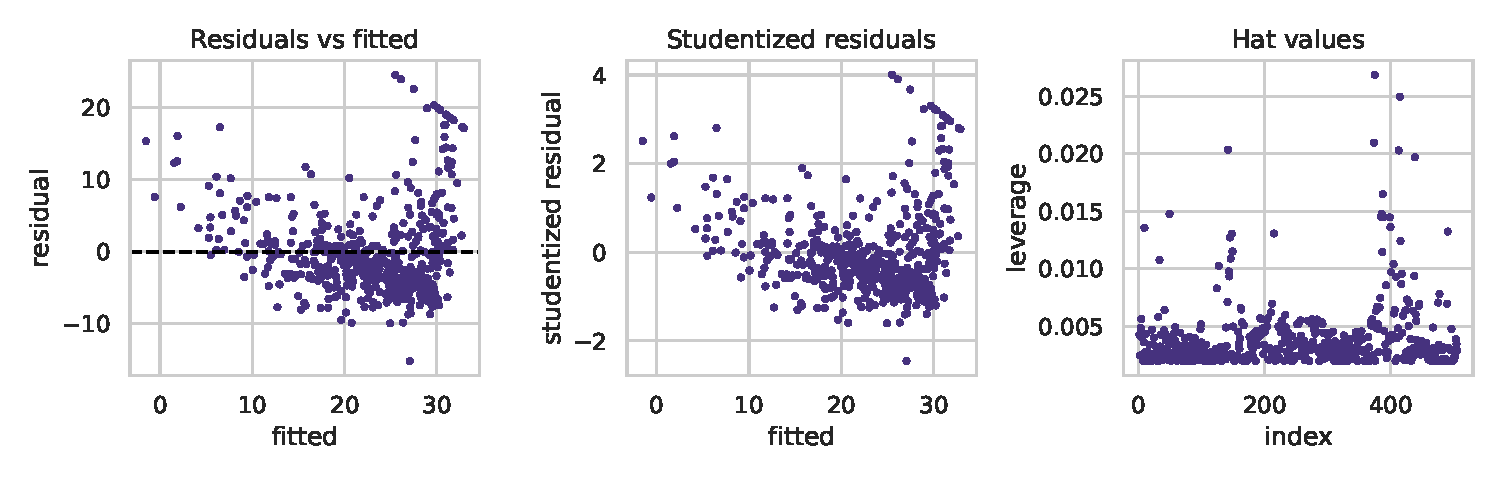
\includegraphics[width=\textwidth]{figures/L18_boston_diag.pdf}
\caption{Boston: residuals and studentized residuals against fitted values (note the curvature), and hat values
by observation index (the maximum is at observation 375).}
\label{fig:L18-diag}
\end{figure}

\subsection{A Monte Carlo simulation}
The code ends with a simulation:
\begin{center}
\begin{minipage}{0.8\textwidth}\small\ttfamily
OneFourthPiSamples = replicate(100, \{ u <- runif(10000); v <- runif(10000);\\
\quad z <- sqrt(u\textasciicircum2 + v\textasciicircum2); sum(z < 1)/10000 \})
\end{minipage}
\end{center}
A point $(U,V)$ uniform on the unit square falls inside the quarter disc $\{u^2+v^2<1\}$ with probability equal to its area,
$\pi/4=0.7854$. Each replicate estimates $\pi/4$ by the proportion of $10\,000$ points inside, with standard error
$\sqrt{(\pi/4)(1-\pi/4)/10000}=0.0041$. With the notebook's seed the $100$ replicates have mean $0.7858$ and
standard deviation $0.0047$. The same idea, repeat an experiment and look at the distribution of an estimate, is how the
notebooks check sampling distributions such as those of \cref{thm:L16-dist}. The instructor uses it for least squares
estimators in Week~7.

\subsection{Computation}
\begin{center}\small
\begin{tabular}{@{}>{\raggedright\arraybackslash}p{7cm}>{\raggedright\arraybackslash}p{8.4cm}@{}}\hline
R & Python (\texttt{statsmodels})\\\hline
\texttt{names(lm.fit)}, \texttt{coef}, \texttt{confint} & \texttt{dir(fit)}, \texttt{fit.params}, \texttt{fit.conf\_int()}\\
\texttt{predict(..., interval="confidence")} & \texttt{fit.get\_prediction(new).summary\_frame()} (\texttt{mean\_ci\_*})\\
\texttt{predict(..., interval="prediction")} & same frame, columns \texttt{obs\_ci\_*}\\
\texttt{plot(lm.fit)} & residual, Q--Q (\texttt{sm.qqplot}), leverage plots\\
\texttt{hatvalues}, \texttt{rstudent} & \texttt{fit.get\_influence().hat\_matrix\_diag}, \texttt{.resid\_studentized\_external}\\
\texttt{replicate(100, \{...\})} & list comprehension with \texttt{rng.uniform}\\\hline
\end{tabular}
\end{center}
See \nb{week05/L18\_computation\_in\_R.ipynb}.

\subsection{Summary}
\begin{itemize}
  \item At $x_0$: confidence interval $\hat Y_0\pm t\,s\sqrt{h_0}$ for the mean, prediction interval $\hat Y_0\pm t\,s\sqrt{1+h_0}$ for a new $Y$, where $h_0=\frac1n+\frac{(x_0-\bar x)^2}{S_{xx}}$.
  \item Leverage $h_{ii}=(\PX)_{ii}\in[0,1]$, $\sum h_{ii}=p$, $\Var\hat e_i=\sigma^2(1-h_{ii})$.
  \item Boston: the residuals show curvature, and the highest leverage is observation $375$.
  \item Monte Carlo: repeat, then summarise the estimates.
\end{itemize}

\subsection{Exercises}
\begin{problem}\label{prob:L18-1}
Show that the prediction interval at $x_0=\bar x$ has half-width $t_{n-2,1-\alpha/2}\,s\sqrt{1+1/n}$.
\end{problem}
\begin{problem}\label{prob:L18-2}
For the four-point data compute all four hat values and check that they sum to $2$.
\end{problem}
\begin{problem}\label{prob:L18-3}
Fit \texttt{medv \textasciitilde\ lstat + I(lstat\textasciicircum2)} and compare $R^2$ and the residual plot with the straight-line fit.
\end{problem}
\begin{problem}\label{prob:L18-4}
Estimate $\pi$ by Monte Carlo with $10^6$ points. How many points are needed for the standard error of the estimate of $\pi$ to be below $0.001$?
\end{problem}

\subsection{Further reading}
ISLR \S3.1--3.3 and Lab~3.6; Weisberg, \emph{ALR}, Chapter~9 (regression diagnostics); Christensen, Chapter~12.


\section*{Solutions to the Exercises of Chapter~\ref{ch:week05}}
\addcontentsline{toc}{section}{Solutions to the exercises}

\paragraph{\Cref{prob:L15-1}.}
Since $\sum_i(x_i-\bar x)=0$, $S_{xy}=\sum_i(x_i-\bar x)(Y_i-\bar Y)=\sum_i(x_i-\bar x)Y_i$. So
$\hat\beta_1=S_{xy}/S_{xx}=\sum_ic_iY_i$. Then $\sum_ic_i=\sum_i(x_i-\bar x)/S_{xx}=0$, and
$\sum_ic_ix_i=\sum_i(x_i-\bar x)x_i/S_{xx}=\sum_i(x_i-\bar x)^2/S_{xx}=1$, again because $\sum_i(x_i-\bar x)\bar x=0$.
It follows that $\EE\hat\beta_1=\sum_ic_i(\beta_0+\beta_1x_i)=\beta_1$ and $\Var\hat\beta_1=\sigma^2\sum_ic_i^2=\sigma^2/S_{xx}$.

\paragraph{\Cref{prob:L15-2}.}
$X\T X=\begin{pmatrix}3&\sum x_i\\\sum x_i&\sum x_i^2\end{pmatrix}=\begin{pmatrix}3&0\\0&2\end{pmatrix}$, so
$\Cov(\hat\beta)=\sigma^2(X\T X)^{-1}=\sigma^2\operatorname{diag}(1/3,\,1/2)$. By \cref{cor:L15-slr},
$\Cov(\hat\beta_0,\hat\beta_1)=-\sigma^2\bar x/S_{xx}$, which is $0$ because the design is centred ($\bar x=0$). Then
$\hat\beta_0=\bar Y$ and $\hat\beta_1$ is a contrast of the $Y_i$, orthogonal to $\one$.

\paragraph{\Cref{prob:L15-3}.}
Write $\hat\beta_0+\hat\beta_1x_0=\bar Y+\hat\beta_1(x_0-\bar x)$. Now
$\Cov(\bar Y,\hat\beta_1)=\sum_i\frac1n c_i\sigma^2=0$ by \cref{prob:L15-1}. Hence
$\Var=\frac{\sigma^2}n+(x_0-\bar x)^2\frac{\sigma^2}{S_{xx}}$. (Equivalently, $\sigma^2 x_0\T(X\T X)^{-1}x_0$ with $x_0=(1,x_0)\T$.)

\paragraph{\Cref{prob:L15-4}.}
$\Var\hat\beta_1=\sigma^2/S_{xx}$, so we maximise $S_{xx}$. For $x_i\in[0,1]$, $x_i^2\le x_i$, so
$S_{xx}=\sum x_i^2-n\bar x^2\le n\bar x-n\bar x^2=n\bar x(1-\bar x)\le n/4$. Equality needs every $x_i\in\{0,1\}$ and
$\bar x=1/2$: put five points at $0$ and five at $1$, giving $S_{xx}=2.5$. Ten equally spaced points give only $S_{xx}=1.019$.
(This design is optimal only if the model is known to be linear. With two support points we cannot check linearity.)

\paragraph{\Cref{prob:L16-1}.}
For the Fort Collins data ($n=93$): $\hat\beta_1=0.2035$, $\widehat{\mathrm{SE}}=0.1310$, $t=1.553$ on $91$ degrees of freedom,
$p=0.124>0.05$. We do not reject $H_0:\beta_1=0$. The $95\%$ CI is $0.2035\pm1.9864\times0.1310=(-0.0568,\,0.4638)$, which
contains $0$. Early-season snowfall tells us little about late-season snowfall.

\paragraph{\Cref{prob:L16-2}.}
$\hat\beta_1=S_{xy}/S_{xx}=r\sqrt{S_{yy}/S_{xx}}$ and $\RSS=S_{yy}-S_{xy}^2/S_{xx}=S_{yy}(1-r^2)$. So
$s^2=S_{yy}(1-r^2)/(n-2)$, and
\[
t=\frac{\hat\beta_1}{s/\sqrt{S_{xx}}}=\frac{r\sqrt{S_{yy}/S_{xx}}\sqrt{S_{xx}}\sqrt{n-2}}{\sqrt{S_{yy}(1-r^2)}}=\frac{r\sqrt{n-2}}{\sqrt{1-r^2}}.
\]
For the snowfall data this gives $1.5528$, the same as the regression $t$.

\paragraph{\Cref{prob:L16-3}.}
The $t$ pivot uses the fact that $(n-p)s^2/\sigma^2=\RSS/\sigma^2\sim\chi^2_{n-p}$, independent of $\hat\beta$. A $t_{n-p}$ variable is
$Z/\sqrt{\chi^2_{n-p}/(n-p)}$, so the divisor must be $n-p$. With $\RSS/n$ the ratio is $\sqrt{n/(n-p)}\,T$, not $t_{n-p}$. It is
also biased: $\EE[\RSS/n]=\frac{n-p}{n}\sigma^2<\sigma^2$ (\cref{thm:L16-s2}). Intervals built from it would be too short.

\paragraph{\Cref{prob:L16-4}.}
$t=(1.4-1)/0.14142=2.828<t_{2,0.975}=4.303$ (two-sided $p=0.106$). We do not reject $\beta_1=1$. This agrees with
$1\in(0.7915,\,2.0085)$ from \cref{ex:L16-hand}.

\paragraph{\Cref{prob:L16-5}.}
With $\sigma^2=0.1$ and $10\,000$ replicates, the notebook finds coverage $0.9499$, within Monte Carlo error
($\pm0.0044$) of $0.95$. The interval is exact for normal errors, whatever $\sigma^2$ and $n$ are.

\paragraph{\Cref{prob:L17-1}.}
Take $x=(1,2,3)$, $y=(3,2,1)$ and fit $y=\beta x$ through the origin. Then $\hat\beta=\sum x_iy_i/\sum x_i^2=10/14=5/7$, the
residuals are $(16,4,-8)/7$, $\RSS=48/7\approx6.857$, and the centred $\TSS=2$. So $1-\RSS/\TSS=-17/7\approx-2.43$.
Without an intercept, $\one\notin\colsp{X}$, the decomposition $\TSS=\mathrm{ESS}+\RSS$ fails, and a line through the
origin can do worse than the constant $\bar y$.

\paragraph{\Cref{prob:L17-2}.}
With an intercept, $\one\in\colsp{X}$, so $\sum_ie_i=0$ and the mean of the $\hat Y_i$ is $\bar Y$. Since $e\perp\hat Y-\bar Y\one$,
\[
\sum_i(Y_i-\bar Y)(\hat Y_i-\bar Y)=\sum_i(\hat Y_i-\bar Y+e_i)(\hat Y_i-\bar Y)=\mathrm{ESS}.
\]
Hence $\operatorname{corr}(Y,\hat Y)^2=\mathrm{ESS}^2/(\TSS\cdot\mathrm{ESS})=\mathrm{ESS}/\TSS=R^2$ by \cref{thm:L17-decomp}.

\paragraph{\Cref{prob:L17-3}.}
$\hat\beta'=c\hat\beta$ and $e'=ce$, so $\RSS'=c^2\RSS$ and $\TSS'=c^2\TSS$. Thus $\RSE'=\abs c\,\RSE$ (RSE is in the units of $Y$),
while $R^2$ is unchanged (it is unit-free).

\paragraph{\Cref{prob:L17-4}.}
The one-way model contains the intercept (as the sum of the group indicators), so $\RSS=\SSW=12=84/7$ and
$\TSS=\SSW+\SSB=84/7+250/7=334/7$. Hence $R^2=\SSB/\TSS=250/334=125/167\approx0.7485$.

\paragraph{\Cref{prob:L18-1}.}
By \cref{prop:L18-intervals} the prediction half-width is $t_{n-2,1-\alpha/2}\,s\sqrt{1+h_0}$ with
$h_0=\frac1n+\frac{(x_0-\bar x)^2}{S_{xx}}$. At $x_0=\bar x$, $h_0=1/n$. This is the narrowest prediction interval.

\paragraph{\Cref{prob:L18-2}.}
$h_i=\frac14+\frac{(x_i-2.5)^2}{5}$ gives $(0.7,0.3,0.3,0.7)$, the diagonal of $\PX$ in \cref{prob:L14-2}. The sum is
$2=\tr\PX=\rank X$ (\cref{prop:L18-hat}).

\paragraph{\Cref{prob:L18-3}.}
The quadratic fit is $\widehat{\texttt{medv}}=42.862-2.3328\,\texttt{lstat}+0.04355\,\texttt{lstat}^2$, with all terms highly
significant. $R^2$ rises from $0.5441$ to $0.6407$ and RSE falls from $6.216$ to $5.524$. The U-shape in the
residual-versus-fitted plot largely disappears, which confirms the non-linearity seen in \cref{fig:L18-diag}.

\paragraph{\Cref{prob:L18-4}.}
$\hat\pi=4\hat p$, where $\hat p$ is the fraction of $m$ uniform points inside the quarter disc. So
$\mathrm{SE}(\hat\pi)=4\sqrt{p(1-p)/m}$ with $p=\pi/4$. For $m=10^6$ this is $0.00164$ (the notebook's estimate is $3.14013$).
The condition $\mathrm{SE}<0.001$ requires $m>16p(1-p)/10^{-6}\approx2.70\times10^6$. Each extra decimal digit costs a factor of $100$ in
sample size.


\end{document}
